\documentclass[11pt]{article}

\usepackage[letterpaper,top=2cm,bottom=2cm,left=1.5cm,right=2cm,marginparwidth=1.75cm]{geometry}
\usepackage{hyperref}
\usepackage{biblatex}
\addbibresource{Bib.bib}
\usepackage{mathtools}
\DeclarePairedDelimiterXPP\BigOSI[2]%
  {\mathcal{O}}{(}{)}{}%
  {\SI{#1}{#2}}
\usepackage{xcolor}
\usepackage{empheq}
\usepackage[most]{tcolorbox}
\usepackage{amsmath}
\usepackage{amssymb}
\usepackage{mathrsfs}
\usepackage[utf8]{inputenc}
\usepackage{graphicx}
\usepackage{float}
\usepackage{parskip}
\usepackage{comment}
%\usepackage{mhchem}
 \usepackage{tabularx}
 \usepackage{titling}
 \usepackage{amsmath,environ}
 \usepackage[explicit]{titlesec}
\usepackage{fancyhdr}
\usepackage{braket}
\usepackage{bbm}
\usepackage{cancel}
\usepackage{simpler-wick}

\setlength{\droptitle}{3em} 

\title{Quantum Field Theory I}
\author{Thomas Brosnan}
\date{Notes taken in Professor Samson Shatashvili class, Michaelmas and Hillary Terms 2024/25}


\newtcbox{\mymath}[1][]{% 
    nobeforeafter, math upper, tcbox raise base,
    enhanced, colframe=blue!30!black,
    colback=blue!30, boxrule=1pt,
    #1}
\tcbset{highlight math style={boxsep=2mm,,colback=blue!0!green!0!red!0!}}

\newenvironment{bux}{\empheq[box=\tcbhighmath]{align}}{\endempheq}
\newenvironment{bux*}{\empheq[box=\tcbhighmath]{align*}}{\endempheq}
\renewenvironment{flalign}{\vspace{-2mm}\empheq[box=\tcbhighmath]{align}}{\endempheq}
\renewenvironment{flalign*}{\vspace{-2mm}\empheq[box=\tcbhighmath]{align*}}{\endempheq}
%\renewenvironment{align}{\vspace{-5mm}\begin{align}}{\end{align}}
%\renewenvironment{align*}{\vspace{-5mm}\begin{align*}}{\end{align*}}
\renewenvironment{alignat}{\empheq{align*}}{\endempheq}



\usepackage{tikz}  % Load TikZ first
\usetikzlibrary{positioning}  % Optional: for advanced positioning
\usetikzlibrary{decorations.markings}

% Declare layers and set their order
\pgfdeclarelayer{nodelayer}
\pgfdeclarelayer{edgelayer}
\pgfsetlayers{nodelayer,edgelayer,main}
\tikzset{
    none/.style = {inner sep=0pt}
}




\newcommand{\hsp}{\hspace{8pt}}

\newcommand*{\sectionFont}{%
  \LARGE\bfseries
}

\newenvironment{eq}{\begin{equation}}{\end{equation}}
    
\numberwithin{equation}{section}

\makeatletter
\let\Title\@title % Copy the title to a new command
\makeatother

%change this RGB value to change the section background colour 
\definecolor{mycolor1}{RGB}{125, 187, 242}
\colorlet{SectionColour}{mycolor1}
%subsection background colour 
\definecolor{mycolor2}{gray}{0.8}
\colorlet{subSectionColour}{mycolor2}
%subsubsection background colour 
\definecolor{mycolor3}{RGB}{255,255,255}
\colorlet{subsubSectionColour}{mycolor3}


\begin{document}

\maketitle

\newpage
\topskip0pt
\vspace*{\fill}
\begin{center}
\Large
    ``If photons study physics, maybe they would come up with spinors'' 

    -Chaolun Wu
\end{center}
\vspace*{\fill} 
\newpage 
\hrule
 \setcounter{tocdepth}{2} % only sections and subsections in Contents
\tableofcontents
\vspace{5mm}
\hrule
% For \section
 \titleformat{\section}[block]{\sectionFont}{}{0pt}{%
 \fcolorbox{black}{SectionColour}{\noindent\begin{minipage}{\dimexpr\textwidth-2\fboxsep-2\fboxrule\relax}\thesection  \hsp #1 {\strut} \end{minipage}}}
% For \subsection
 \titleformat{\subsection}[block]{\bfseries}{}{0pt}{%
 \fcolorbox{black}{subSectionColour}{\noindent\begin{minipage}{\dimexpr\textwidth-2\fboxsep-2\fboxrule\relax}\thesubsection  \hsp #1 {\strut} \end{minipage}}}
% For \section*
 \titleformat{name=\section, numberless}[block]{\sectionFont}{}{0pt}{%
 \fcolorbox{black}{SectionColour}{\noindent\begin{minipage}{\dimexpr\textwidth-2\fboxsep-2\fboxrule\relax} #1 {\strut} \end{minipage}}}
  % For \subsection*
 \titleformat{name=\subsection, numberless}[block]{\bfseries}{}{0pt}{%
 \fcolorbox{black}{subSectionColour}{\noindent\begin{minipage}{\dimexpr\textwidth-2\fboxsep-2\fboxrule\relax} #1 {\strut} \end{minipage}}}
 % For \subsubsection
 \titleformat{\subsubsection}[block]{\bfseries}{}{0pt}{%
 \fcolorbox{black}{subsubSectionColour}{\noindent\begin{minipage}{15cm}\thesubsubsection \hsp #1 {\strut} \end{minipage}}}
  % For \subsubsection*
 \titleformat{name=\subsubsection, numberless}[block]{\bfseries}{}{0pt}{%
 \fcolorbox{black}{subsubSectionColour}{\noindent\begin{minipage}{15cm} #1 {\strut} \end{minipage}}}
\newpage 
%header 
\pagestyle{fancy}
\fancyhf{} % Clear all header and footer fields
\fancyhead[L]{\Title}
\fancyhead[R]{\nouppercase{\leftmark}}
\fancyfoot[C]{-~\thepage~-}
\renewcommand{\headrulewidth}{1pt}





%starting document 
\normalsize
\newpage 

\section{The Need for Fields}
In this section we will see where regular quantum mechanics fails and what we need to do to fix it. 

\subsection{Non-relativistic free particle}

\begin{itemize}
  \item We can recall from QM that the probability of a particle at point $x$ at time $t$ propagating to $x'$ at time $t'$ is given by:
  \begin{equation}
  \label{propagator}
    \bra{x} e^{-iH(t-t')} \ket{x'}
  \end{equation}
  Here $H$ is the Hamiltonian. For a Non-relativistic free particle we have that $H = \hat{\textbf{P}}^2/2m$. We can then go about solving dor this propagator with this Hamiltonian in the usual way. This involves inserting the identity $\int \frac{d^3p}{(2\pi)^3}\ket{p}\bra{p} = \mathbb{I}$ into the above propagator \ref{propagator}before the $\ket{x'}$

  \begin{equation*}
      \bra{x} e^{-iH(t-t')} \ket{x'}  = \int \frac{d^3p}{(2\pi)^3}\bra{x}e^{-i\frac{\hat{\textbf{P}}^2}{2m}(t-t')}\ket{p}\braket{p|x'}
  \end{equation*}
  Then if we recall that $\braket{p|x'} = e^{-i\textbf{p}\cdot\textbf{x}'}$, $\braket{x|p} = e^{i\textbf{p}\cdot\textbf{x}}$ and $e^{-i\frac{\hat{\textbf{P}}^2}{2m}(t-t')}\ket{p} = e^{-i\frac{p^2}{2m}(t-t')}\ket{p}$. We get:

  \begin{flalign*}
    \bra{x} e^{-iH(t-t')} \ket{x'} & = \int \frac{d^3p}{(2\pi)^3}e^{-i\frac{p^2}{2m}(t-t')}e^{i\textbf{p}\cdot(\textbf{x}-\textbf{x}')} \\
    & = \left(\frac{m}{2\pi i(t-t')}\right)^{3/2}e^{im\frac{(\textbf{x}-\textbf{x}')^2}{2(t-t')}}
  \end{flalign*}
  \item What this is saying, is that for any two points $x$ and $x'$, no matter how far they are separated, have a non-zero probability of propagation from one to another. But this is direct contrast with what we know from special relativity! Two points separated by enough distance so that there space time interval, $\Delta s^2 = (t-t')^2 -|\textbf{x}-\textbf{x}'|^2$ is negative, i.e. space like. Which would require a propagation speed faster then light. 
\end{itemize}
\subsubsection{Non-trivial Gaussian integral}
\begin{itemize}
  \item In the above calculation we have to evaluate the following integral: 
  \begin{align*}
    \int_{\infty}^{\infty}e^{-(p+ia)^2}dp 
  \end{align*}
  Now we may think we can just make the substitution $u=p+ia$, but since we are involving complex numbers, we get a non trivial problem with the limits, as they change to $\infty-ia$ and $\infty+ia$. What we can do instead is calculate the integral of a closed contour. Since the integrand above has no poles, we know that any closed contour on the complex plain should evaluate to 0. What we will do is then modify the limits of our integral to be from $-q$ to $q$, we will take the limit at the end to recover what we got. We can then integrate along the following path: We start at $q+ia$ and move to $-q+ia$, then from $-q+ia$ to $-q$, from  $-q$ to $q$ and from $q$ to $q+ia$. This is a closed contour, that we will call $C$. We then have that:
  \begin{align*}
        0=\int_{C}e^{-z^2}dz = \int_{q+ia}^{-q+ia}e^{-(x)^2}dx+\int_{a}^{0}e^{-(-q+iy)^2}dy+\int_{-q}^{q}e^{-x^2}dx+\int_{0}^{a}e^{-(q+iy)^2}dy
     \end{align*}  
     We can then immediately argue that the second and fourth integrals should vanish when we send $q$ to infinity. Then the first integral we can reverse the limits and pick up a minus sign so: 
     \begin{align*}
        \int_{-q+ia}^{q+ia}e^{-(x)^2}dx = \int_{-q}^{q}e^{-x^2}dx = \sqrt{\pi}
      \end{align*} 
      And then finally now we can make a $u$-substitution of the LHS, to get back our original integral! So we can see in this case that since the two ends of this contour vanished in the arge $q$ limit we are essentially able to move our contour up and down to get the regular Gaussian integral.  
\end{itemize}

\subsection*{Relativistic free particle}
\begin{itemize}
  \item But we can chalk this up to a mistake. We were not considering the Hamiltonian of a \textbf{relativistic} free particle. That is, with the Hamiltonian $H  = \sqrt{\textbf{P}^2 + m^2}$. The propagator in a similar manner to before then becomes: 
  \begin{equation*}
  \begin{split}
     \bra{x} e^{-i\sqrt{\textbf{P}^2 + m^2}(t-t')} \ket{x'} & = \int \braket{x|p}  e^{-i\sqrt{\textbf{P}^2 + m^2}(t-t')}  \braket{p|x'}\frac{d^3p}{(2\pi)^3} \\
     & = \int \frac{d^3p}{(2\pi)^3}  e^{-i\sqrt{p^2 + m^2}(t-t')+ i\textbf{p}\cdot(\textbf{x}-\textbf{x}')} 
  \end{split}
  \end{equation*}
  We can then parametrize the angle part of this integral by letting $\theta$ be the angle between $\textbf{p}$ and $(\textbf{x}-\textbf{x}')$, we can also further parametrize this with $\eta = \cos{\theta}$:
  \begin{equation*}
  \begin{split}
  \bra{x} e^{-i\sqrt{\hat{\textbf{P}}^2 + m^2}(t-t')} &\ket{x'}  = \int_{0}^{\infty} \frac{p^2dp}{(2\pi)^2}  \int_{-1}^{1} d \eta e^{-i\sqrt{p^2 + m^2}(t-t')+ ip|\textbf{x}-\textbf{x}'|\eta} \\
   = \int_{0}^{\infty} \frac{p^2dp}{(2\pi)^2}& e^{-i\sqrt{p^2 + m^2}(t-t')} \frac{1}{ip|\textbf{x}- \textbf{x}'|}\left(e^{ ip|\textbf{x}-\textbf{x}'|}-e^{- ip|\textbf{x}-\textbf{x}'|} \right)
  \end{split}
  \end{equation*}
  We can then turn this into an integral from $-\infty$ to $\infty$ with a factor of 2:
  \begin{equation}
  \label{Rel_propagator}
  \begin{split}
 = \frac{-i}{2\pi^2|\textbf{x}- \textbf{x}'|}\int_{0}^{\infty}pdp~e^{-i\sqrt{p^2 + m^2}(t-t')+ip|\textbf{x}-\textbf{x}'|}
  \end{split}
  \end{equation}
\end{itemize}
\subsubsection{Laplace steepest decent}
\begin{itemize}
  \item We can then use a useful approximation of integrals of this form by expanding around critical points. That is points $x_0$ where $f'(x_0)= 0$. The approximation is as follows, for a critical point $x_0$ of $f(x)$:
  \begin{flalign*}
\int_{-\infty}^{\infty}&h(x)e^{Af(x)}dx =  \int_{-\infty}^{\infty}h(x)e^{A\left[f(x_0) + \frac{1}{2}f''(x_0)(x-x_0)^2+\mathcal{O}((x-x_0)^3)\right]}dx \\ 
 \approx   h(x_0)e^{Af(x_0)}&\int_{-\infty}^{\infty}e^{-A\frac{1}{2}|f''(x_0)|(x-x_0)^2}dx = \sqrt{\frac{2\pi}{A|f''(x_0)|}}h(x_0)e^{Af(x_0)} 
  \end{flalign*}
  \item Where we have assumed $x_0$ is a global maxima so that $f''(x_0) \leq 0$. This approximation works well as the exponential ensures that any small deviation from $x_0$ contributes very little to the integral. It of course depends also on $h(x)$ being "well behaved".


  \item Back to the relevant integral \ref{Rel_propagator}, we can see that for us $f(p) = -i\sqrt{p^2 + m^2}(t-t')+ip|\textbf{x}-\textbf{x}'|$ and $h(p) = p$. So we find the stationary point of $f(p)$ via $f'(p_0)=0$: 
  \begin{equation*}
  \begin{split}
      f'(p_0) = \frac{-p_0(t-t')}{\sqrt{p_0^2+m^2}}+|\textbf{x}-\textbf{x}'| =0 \implies p_0^2 = \frac{m^2|\textbf{x}-\textbf{x}'|^2}{(t-t')^2-|\textbf{x}-\textbf{x}'|^2}
      \end{split}
    \end{equation*}  
    Then we can evaluate $f(p_0)$:
    \begin{equation*}
    \begin{split}
      f(p_0) & = -i\sqrt{\frac{m^2|\textbf{x}-\textbf{x}'|^2}{(t-t')^2-|\textbf{x}-\textbf{x}'|^2}+m^2}(t-t')+i\sqrt{\frac{m^2|\textbf{x}-\textbf{x}'|^2}{(t-t')^2-|\textbf{x}-\textbf{x}'|^2}} \\
      & = -\frac{m(|\textbf{x}-\textbf{x}'|^2-(t-t')^2)}{\sqrt{|\textbf{x}-\textbf{x}'|^2-(t-t')^2}} = -m\sqrt{|\textbf{x}-\textbf{x}'|^2-(t-t')^2}
    \end{split}
    \end{equation*}
    Where we have used the fact that we are considering probabilities outside the light-cone, i.e. where $|\textbf{x}-\textbf{x}'| > (t-t')$, so that the square root $ \sqrt{(t-t')^2-|\textbf{x}-\textbf{x}'|^2}=i\sqrt{|\textbf{x}-\textbf{x}'|^2-(t-t')^2}$ . 

    \item With this we can now use Laplace's steepest decent integral approximation to write:
    \begin{flalign*}
    \bra{x} e^{-i\sqrt{\hat{\textbf{P}}^2 + m^2}(t-t')} \ket{x'} \propto h(p_0)e^{f(p_0)} \propto e^{-\sqrt{|\textbf{x}-\textbf{x}'|^2-(t-t')^2}}
    \end{flalign*}
    This again does not solve our problem, we have that there is a non-zero probability of propagating to outside the light-cone. Some more radical approach is needed to solve this problem. 
\end{itemize}

\subsection{Field theory EoM}
\begin{itemize}
  \item The  Idea will be to go from dealing with particle, to waves. For this we need to generalize our idea of action being the integral of a Lagrangian over time to being the integral of a Lagrange density over time and space as a field is spread out, not localized. This means:
  \begin{equation*}
    S = \int L(q_i,\dot{q}_i,t)dt \rightarrow \int d^4x\mathcal{L}(\varphi(\textbf{x},t),\partial_{\mu} \varphi(\textbf{x},t))
  \end{equation*}
  We then have to vary this action to set $\delta S = 0$:
  \begin{equation*}
    \delta S = \int d^4x \left(\frac{\delta \mathcal{L}}{\delta \varphi}\delta \varphi  - \frac{\delta \mathcal{L}}{\delta \partial_{\mu} \varphi}\delta\partial_{\mu}\varphi\right) = \int d^4x \left(\frac{\delta \mathcal{L}}{\delta \varphi}  - \partial_{\mu}\left(\frac{\delta \mathcal{L}}{\delta \partial_{\mu} \varphi}\right)\right)\delta \varphi 
  \end{equation*}
  \begin{flalign}
  \label{EoM}
    \implies \frac{\delta \mathcal{L}}{\delta \varphi}  - \partial_{\mu}\frac{\delta \mathcal{L}}{\delta \partial_{\mu} \varphi} = 0 
  \end{flalign}
  Where we have integrated by parts the second term.
\end{itemize}

\subsection{Non-degenerate Lagrangian}{\label{Non-degenerate Lagrangian}}
\begin{itemize}
  \item It is often the case, that when we have constructed our Lagrangian, that we would like to perform a Legendre transform from the variables $q$ and $\dot{q}$, to $q$ and $p$. This is gives us our Hamiltonian and takes the form $H =\sum_i p_i \dot{q}_i  - L(q,\dot{q})$. In doing this we are required to solve for $\dot{q}$ in terms of $q$ and $p$. But this is not always possible, for example given the Lagrangian $L \propto \dot{q} \implies p = \frac{\partial L}{\partial q} = 1$, so we are unable to solve for $\dot{q}(p,q)$. It turn out the condition for us to always be able to solve for $\dot{q}$ is as follows:

  If we denote the matrix $M_{ij} = \frac{\partial^2 L}{\partial\dot{q}^i\partial\dot{q}^j}$, then the condition becomes, we can solve for $\dot{q}_{i} \iff \text{det}(M) \neq 0$. The Lagrangian can then be written as:

  \begin{equation*}
  L = \sum_{i,j}M_{ij}\partial\dot{q}^i\partial\dot{q}^j, ~~~ \text{and}~~~ \dot{q}^i  = \sum_{j}M^{-1}_{ij}p_j
  \end{equation*}
  This is called a Non-degenerate Lagrangian. 
\end{itemize}

\subsection{Hamiltonian field theory} 
\begin{itemize}
  \item We wish to find a Hamiltonian for our field theory. The best way to go about extending our definition of $H =\sum_i p_i \dot{q}_i  - L(q,\dot{q})$, is to think of space as a discretized space, as we had the co-ordinates $q$ indexed by $i$. We can then calculate:

  \begin{equation*}
  p(\textbf{x}) = \frac{\partial L}{\partial \dot{\phi}} = \frac{\partial }{\partial \dot{\phi}(\textbf{x})}\sum_{\textbf{y}}\mathcal{L}(\phi(\textbf{y}),\dot{\phi}(\textbf{y}))d^3y = \pi(\textbf{x})d^3x. 
  \end{equation*}
  Where:
  \begin{flalign}
  \label{pi}
  \pi(\textbf{x}) = \frac{\partial \mathcal{L}}{\partial \dot{\phi}(\textbf{x})}
  \end{flalign}
  This is called the \emph{momentum density} conjugate to $\phi(\textbf{x})$. We can now write the Hamiltonian as:
  \begin{equation*}
    H = \sum_{\textbf{x}}p(\textbf{x})\dot{\phi}(\textbf{x}) - L
  \end{equation*}
  Which in the continuum limit becomes:
  \begin{flalign}
\label{Hamiltonian}
     H = \int d^3x[\pi(\textbf{x})\dot{\phi}(\textbf{x}) - \mathcal{L}] \equiv \int d^3x\mathcal{H} 
   \end{flalign} 
\end{itemize}


\subsection{Noether's Theorem}
\begin{itemize}
  \item We are used to Noether's Theorems relation between symmetries and conservation in the context of particles. We will now discuss this in the context of fields. If we have an infinitesimal transformation of fields taking the form:
  \begin{equation*}
     \phi(x) \rightarrow \phi'(x) = \phi(x) + \alpha\Delta\phi(x)
   \end{equation*} 
Here $\alpha$ is small. This transformation is a symmetry if it results in the same EoM, i.e. leaves the action unchanged. This means the Lagrangian must be the same up to the addition of a total derivative, which in this context is the 4-gradient:
\[
      \mathcal{L}(x) \rightarrow \mathcal{L}(x) + \alpha \partial_{\mu}\mathcal{J}^{\mu}(x)
\]
    Where $\mathcal{J}^{\mu}$ is some 4-vector. We can then find the expected form of $\Delta \mathcal{L}(\phi,\partial_{\mu}\phi )$:
    \begin{align*}
     \alpha \Delta \mathcal{L} & = \frac{\partial \mathcal{L}}{\partial \phi}(\alpha \Delta \phi) + \left(\frac{\partial \mathcal{L}}{\partial (\partial_{\mu}\phi)}\right)\partial_{\mu}(\alpha\Delta\phi) \\
    &  = \alpha \partial_{\mu}\left(\frac{\partial \mathcal{L}}{\partial(\partial_{\mu}\phi)}\Delta \phi\right)+\alpha\left[\frac{\partial\mathcal{L}}{\partial \phi} - \partial_{\mu}\left(\frac{\partial \mathcal{L}}{\partial(\partial_{\mu}\phi)}\right)\right]\Delta \phi 
    \end{align*}
    We can then recognize that the second term vanished via our EoM \ref{EoM}, so we can set the remaining term to $\alpha \partial_{\mu}\mathcal{J}^{\mu}(x)$, which is equivalent to:
\begin{flalign}
\label{Noether}
  \partial_{\mu}j^{\mu}(x) = 0, ~~~~\text{for} ~~j^{\mu}(x) = \frac{\partial \mathcal{L}}{\partial(\partial_{\mu}\phi)}\Delta \phi - \mathcal{J}^{\mu}
\end{flalign}
\item If the symmetry involves more then one field the first term above should be a sum of those terms, for the different fields. This conservation law also implies that there is a charge constant in time namely:
\begin{flalign}
\label{charge}
Q \equiv \int j^{0} d^3x
\end{flalign}
\end{itemize}
\subsection{Stress-Energy Tensor}
\begin{itemize}
\item We can also consider transformations of space itself, for example, translations or rotations. This takes the for $x^{\mu} \rightarrow x^{\mu} - a^{\mu}$, which has the following affect on the fields (when infinitesimal): 

\[ 
  \phi(x) \rightarrow \phi(x+a) = \phi(x) + a^{\mu}\partial_{\mu}\phi(x)
 \]
The Lagrangian must also transform in the same way as it is also a scalar:
\[ 
  \mathcal{L}(x) \rightarrow \mathcal{L}(x+a) = \mathcal{L}(x) + a^{\nu}\partial_{\mu}(\delta^{\mu}_{\nu}\mathcal{L}(x))
 \]
 We can then recognize the $\delta^{\mu}_{\nu}\mathcal{L}(x)$ as $ \sim \mathcal{J}^{\mu}$ from \ref{Noether}, however since the change in the scalar field became a vector $\Delta \phi \rightarrow \partial_{\mu}\phi(x)$, then we must add a second index to our $\mathcal{J}^{\mu} \rightarrow \mathcal{J}^{\mu}_{~\nu}$. This is for the reason for the $\delta_{\nu}^{\mu}$ in the above expression and means our conserved vector $j^{\mu}$ becomes a conserved tensor of the form:

 \begin{flalign*}
      \partial_{\mu}T^{\mu}_{~\nu}(x) = 0, ~~~~\text{for} ~~T^{\mu}_{~\nu}(x) = \frac{\partial \mathcal{L}}{\partial(\partial_{\mu}\phi)}\partial_{\nu}\phi - \delta^{\mu}_{\nu}\mathcal{L}
  \end{flalign*} 
  This is the \emph{Stress-Energy Tensor} also called the \emph{Energy-Momentum Tensor}. We can then notice that the conserved charge associated with the time translations is nothing more then out Hamiltonian:
  \[
\int T^{00}d^3x = \int\left(\frac{\partial \mathcal{L}}{\partial\dot{\phi}}\dot{\phi} - \mathcal{L}\right)d^3x = \int \mathcal{H}d^3x = H  
  \] 
  Similarly for space translation the conserved charges are the physical momenta, not to be confused with the canonical momentum.
  \[  
  \int T^{0i}d^3x = \int \mathcal{P}_id^3x = P_i 
  \] 
\end{itemize}
\newpage
\section{The Klein-Gordon Field}
\begin{itemize}
  \item We ease ourselves into the concepts of quantum fields with the discussion of the Klein-Gordon field. This is one of the simplest types of fields and its use becomes obvious when we see the EoM, which is just the Schr\"odinger equation but made relativistic by replacing $\hat{\textbf{p}}^2/2m \rightarrow \sqrt{\hat{\textbf{p}}^2 + m^2}$. We will see more of this later.

     \item The Lagrange density for the Klein-Gordon field takes the form:
     \begin{equation}
       \label{KG field}
       \mathcal{L} = \frac{1}{2}\partial_{\mu} \phi \partial^{\mu}\phi -\frac{m^2}{2}\phi^2
     \end{equation}   
From this we can calculate the momentum density via \ref{pi} to get $\pi = \dot{\phi}$. And thus via \ref{Hamiltonian} the Hamiltonian density is:
\begin{equation}
\label{KG_Ham}
  \mathcal{H} = \frac{1}{2}\left(\pi^2 +(\nabla\phi)^2+m^2\phi^2\right) 
\end{equation}
\item The equations of motion can also be calculated easily via \ref{EoM} resulting in the \emph{Klein-Gordon equation}:
\begin{flalign}
\label{KG eq}
  (\partial_{\mu}\partial^{\mu}+m^2)\phi  = 0
\end{flalign} 
This $\partial_{\mu}\partial^{\mu}$ is often denoted $\Box$. As an aside, if we "make" the Schr\"odinger equation relativistic, i.e. $\textbf{p}^2 + m^2 = E^2$ and use the definition of the operators $ i\partial_t\psi= E\psi $ and $\hat{\textbf{p}} = -i\nabla$, so:  $-\nabla^2 + m^2 = -\partial^2_t$, recovering us the above Klein-Gordon equation.  
\end{itemize}

\subsection{Second Quantization}
\begin{itemize}
  \item We will now see if we can ``quantize'' this field. What we can do to help figure out how to do this is to take inspiration from the quantization of the single particle Harmonic oscillator in QM. This works nicely as we can see the Lagrangian density for the Klein-Gordon field \ref{KG field} resembles that of the harmonic oscillator. By quantize here we mean to reinterpret the dynamical variables as operators that obey canonical commutation relations, like $[p_i,q_j] = i\delta_{i,j},~[q_i,q_j] = 0 = [p_i,p_j]$. Instead however $\phi$ and $\pi$ will become our operators and we will require that $[\phi(\textbf{x}),\pi(\textbf{y})] = i \delta(\textbf{x}-\textbf{y}),~ [\phi(\textbf{x}),\phi(\textbf{y})] = 0 = [\pi(\textbf{x}),\pi(\textbf{y})]$. This procedure is often called \emph{Second Quantization} to distinguish it from the old one particle version. 
  
  \item Our goal is to now find the spectrum of the Hamiltonian. We start by taking our field $\phi(\textbf{x})$ and writing it in terms of its Fourier transform to momentum (p)-space
\[
  \phi(\textbf{x}) = \int \frac{d^3p}{(2\pi)^3}\phi(\textbf{p})e^{i\textbf{p}\cdot\textbf{x}}
\]
Here we also require that $\phi(\textbf{x},t)$ is real so $\phi^{\ast}(\textbf{p}) = \phi(-\textbf{p})$ Then using the Klein-Gordon equation \ref{KG eq} we get the condition:
\[
  \left[\partial_t^2 + p^2+m^2\right]\phi(\textbf{p}) = 0 
\]
Where we have acted the $-\partial^2_{i}$ from $\Box$ on the exponential to pull out the $p^2$ This equation of motion is the same as that of a harmonic oscillator with frequency $\omega_{\textbf{p}} = \sqrt{p^2+m^2}$. 

\item We now recall from QM that in order to solve the harmonic oscillator we introduced the creation ($\hat{a}^{\dagger}$) and annihilation ($\hat{a}$) operators, so that we could write $\hat{q} = \frac{1}{\sqrt{2 \omega}}(\hat{a}+\hat{a}^{\dagger})$ and $\hat{p} = -i\sqrt{\frac{\omega}{2}}(\hat{a}-\hat{a}^{\dagger})$. This then meant the Hamiltonian took the form $H = \frac{1}{2}(\hat{p}^2+\omega^2\hat{q}^2) = \omega(\hat{a}^{\dagger}\hat{a}+\frac{1}{2})$ and also that the commutators  were: $[H,\hat{a}^{\dagger}] = \omega \hat{a}^{\dagger}$ , $[H,\hat{a}] = -\omega \hat{a}$ and $[a,a^{\dagger}] =\mathcal{I}$. 
 
\item This can be done for our field $\phi$, except we have to consider that $\hat{q} = \frac{1}{\sqrt{2 \omega}}(\hat{a}+\hat{a}^{\dagger})$ is a function of momentum as for us we have $\omega_{\textbf{p}} = \sqrt{p^2+m^2}$. We can then recall that since we expect $\phi$ to be real we require that $\phi^{\dagger}(\textbf{p}) = \phi(-\textbf{p})$, this means we should have $\phi(\textbf{p}) \propto a_{\textbf{p}}+a^{\dagger}_{-\textbf{p}}$ as then $\phi(\textbf{p})^{\dagger} \propto a_{\textbf{p}}^{\dagger}+ a_{-\textbf{p}} \propto \phi(-\textbf{p})$. This means our corresponding expression for $\phi$ should take the form:
\begin{equation}
\label{phi_1}
  \phi(\textbf{x}) = \int \frac{d^3p}{(2\pi)^3}\frac{1}{\sqrt{2\omega_{\textbf{p}}}}\left(a_{\textbf{p}}+a^{\dagger}_{-\textbf{p}}\right)e^{i\textbf{p}\cdot\textbf{x}} 
\end{equation} 
\begin{equation}
\label{pi_1}
  \pi(\textbf{x}) = -i\int \frac{d^3p}{(2\pi)^3}\sqrt{\frac{\omega_{\textbf{p}}}{2}}\left(a_{\textbf{p}}-a^{\dagger}_{-\textbf{p}}\right)e^{i\textbf{p}\cdot\textbf{x}} 
\end{equation} 
We can also think of this expression as each Fourier mode of the field being treated as an independent oscillator with its own $a$ and $a^{\dagger}$ (which will also be a function of the momentum). We can then isolate the second term in this integral and change $\textbf{p}$ to $-\textbf{p}$, since we are integrating over all momentum space, this just results in the signs of the $p$'s in the term changing so we can write:

\begin{flalign}
\label{phi_2}
  \phi(\textbf{x}) = \int \frac{d^3p}{(2\pi)^3}\frac{1}{\sqrt{2\omega_{\textbf{p}}}}\left(a_{\textbf{p}}e^{i\textbf{p}\cdot\textbf{x}}+a^{\dagger}_{\textbf{p}}e^{-i\textbf{p}\cdot\textbf{x}}\right) 
\end{flalign}
In a similar manner the momentum density can be written as:

\begin{flalign}
\label{pi_2}
  \pi(\textbf{x}) = -i\int \frac{d^3p}{(2\pi)^3}\sqrt{\frac{\omega_{\textbf{p}}}{2}}\left(a_{\textbf{p}}e^{i\textbf{p}\cdot\textbf{x}}-a^{\dagger}_{\textbf{p}}e^{-i\textbf{p}\cdot\textbf{x}}\right) 
\end{flalign}
\end{itemize}
\subsubsection{Commutators}
\begin{itemize}
\item We can then go about checking the commutator $[\phi(\textbf{x}),\pi(\textbf{x}')]= i \delta(\textbf{x}-\textbf{y})$ which should be equivalent to the the new creation and annihilation operators satisfying $[a_{\textbf{p}},a^{\dagger}_{\textbf{p}'}] = (2 \pi)^{3}\delta(\textbf{p}-\textbf{p}')$. Using the above definitions \ref{phi_1} and \ref{pi_1} for this calculation is easier, resulting in:
\begin{equation}
\begin{split}
  [\phi(\textbf{x}),\pi(\textbf{x}')] & = -\frac{i}{2}\int \frac{d^3pd^3p'}{(2\pi)^6}\sqrt{\frac{\omega_{\textbf{p}'}}{\omega_{\textbf{p}}}}\left[-a_{\textbf{p}}a^{\dagger}_{\textbf{-p}'} + a^{\dagger}_{\textbf{-p}}a_{\textbf{p}'}-(-a^{\dagger}_{\textbf{p}'}a_{\textbf{-p}} + a_{\textbf{p}}a^{\dagger}_{\textbf{-p}'})\right]e^{i(\textbf{p}\cdot \textbf{x}+\textbf{p}'\cdot \textbf{x}')} \\ 
  &  = -\frac{i}{2}\int \frac{d^3pd^3p'}{(2\pi)^6}\sqrt{\frac{\omega_{\textbf{p}'}}{\omega_{\textbf{p}}}}\left[[a^{\dagger}_{\textbf{-p}},a_{\textbf{-p}'}]-[a_{\textbf{p}},a^{\dagger}_{\textbf{-p}'}]\right]e^{i(\textbf{p}\cdot \textbf{x}+\textbf{p}'\cdot \textbf{x}')}  \\ 
   & =  -\frac{i}{2}\int \frac{d^3pd^3p'}{(2\pi)^6}\sqrt{\frac{\omega_{\textbf{p}'}}{\omega_{\textbf{p}}}}(2\pi)^3\left[-\delta(\textbf{p}'+\textbf{p}) -\delta(\textbf{p}+\textbf{p}') \right]e^{i(\textbf{p}\cdot \textbf{x}+\textbf{p}'\cdot \textbf{x}')}  \\ 
   & = i\int \frac{d^3p}{(2\pi)^3}e^{i\textbf{p}\cdot( \textbf{x} -\textbf{x}')} = i\delta(\textbf{x} -\textbf{x}')  
  \end{split}
  \end{equation}  
  Where we have used the fact that $\omega_{\textbf{p}}=\omega_{\textbf{-p}}$ by definition. We can then also calculate the Hamiltonian via \ref{KG_Ham}:
  \begin{equation*}
    \begin{split}
      H  = \frac{1}{2}\int &d^3x\int\frac{d^3pd^3p'}{(2\pi)^6}\left[\frac{-\sqrt{\omega_{\textbf{p}}\omega_{\textbf{p}'}}}{2}\left(a_{\textbf{p}}-a^{\dagger}_{\textbf{-p}}\right)\left(a_{\textbf{p}'}-a^{\dagger}_{\textbf{-p}'}\right)\right. \\
       & \left. + \frac{-\textbf{p}\cdot \textbf{p}'+m^2}{2\sqrt{\omega_{\textbf{p}}\omega_{\textbf{p}'}}}\left(a_{\textbf{p}}+a^{\dagger}_{\textbf{-p}}\right)\left(a_{\textbf{p}'}+a^{\dagger}_{\textbf{-p}'}\right)\right]e^{i\textbf{x}\cdot(\textbf{p}+\textbf{p}')} \\
    \end{split}
  \end{equation*}
  We can then notice that the $\textbf{x}$ part of this integral creates a delta function $\int d^3xe^{i\textbf{x}\cdot(\textbf{p}+\textbf{p}')} = (2\pi)^{3}\delta(\textbf{p}+\textbf{p}')$, so $\textbf{p}= - \textbf{p}'$. This allows us to write:
  \begin{equation*}
    \begin{split}
    H  & = \frac{1}{4}\int\frac{d^3p}{(2\pi)^3}\omega_{\textbf{p}}\left[-\left(a_{\textbf{p}}-a^{\dagger}_{\textbf{-p}}\right)\left(a_{\textbf{-p}}-a^{\dagger}_{\textbf{p}}\right) + \left(a_{\textbf{p}}+a^{\dagger}_{\textbf{-p}}\right)\left(a_{\textbf{-p}}+a^{\dagger}_{\textbf{p}}\right) \right]  \\ 
    & = \frac{1}{2}\int\frac{d^3p}{(2\pi)^3}\omega_{\textbf{p}}\left[a_{\textbf{p}}a^{\dagger}_{\textbf{p}}+a^{\dagger}_{\textbf{-p}}a_{-\textbf{p}}\right]
 \end{split}
  \end{equation*}
  We can then for this second term do the same trick of changing $\textbf{p} \rightarrow -\textbf{p}$, which does not affect the integral's value as $\omega_{\textbf{p}} = \omega_{-\textbf{p}}$. Then also using the fact that $a^{\dagger}_{\textbf{p}}a_{\textbf{p}} = a_{\textbf{p}}a^{\dagger}_{\textbf{p}}-[a_{\textbf{p}},a^{\dagger}_{\textbf{p}}]$ we get the final result that:

  \begin{flalign}
  \label{Ham_SH}
  H = \int \frac{d^3p}{(2\pi)^3}\omega_{\textbf{p}}\left[a_{\textbf{p}}a^{\dagger}_{\textbf{p}}-\frac{1}{2}[a_{\textbf{p}},a^{\dagger}_{\textbf{p}}]\right]
  \end{flalign}
  If we stop to think about the second term in this expression we realize something strange, $[a_{\textbf{p}},a^{\dagger}_{\textbf{p}}] = (2\pi)^3\delta(0)$, which is and infinite constant (constant as in it wont affect any state we act $H$ on). But since this is constant we can never measure it experimentally as we only ever measure the energy shift between two different energies. We can also think of this as the zero point energy for each point in space, except that we made this space continuous resulting in infinite many oscillator ground states, so what did we expect really? This means we can ignore the second term in \ref{Ham_SH}.

   To make sure everything is consistent we also check the commutators, $[H,a_{\textbf{p}}^{\dagger}] = \omega a^{\dagger}_{\textbf{p}}$ , $[H,a_{\textbf{p}}] = -\omega a_{\textbf{p}}$:
   \begin{equation*}
      \begin{split}
        [H,a_{\textbf{p}}] & = \int \frac{d^3p'}{(2\pi)^3}\omega_{\textbf{p}'}\left[a_{\textbf{p}'}a^{\dagger}_{\textbf{p}'}a_{\textbf{p}}-a_{\textbf{p}}a^{\dagger}_{\textbf{p}'}a_{\textbf{p}'}\right] \\
        & = \int \frac{d^3p'}{(2\pi)^3}\omega_{\textbf{p}'}\left[a_{\textbf{p}'}a_{\textbf{p}}a^{\dagger}_{\textbf{p}'}-a_{\textbf{p}'}[a_{\textbf{p}},a^{\dagger}_{\textbf{p}'}]-a_{\textbf{p}}a_{\textbf{p}'}a^{\dagger}_{\textbf{p}'}\right] \\
        & = -\omega_{\textbf{p}}a_{\textbf{p}} 
      \end{split}
   \end{equation*}
   Here we have used the fact that $[a_{\textbf{p}},a_{\textbf{p}'}]= 0 = [a^{\dagger}_{\textbf{p}},a^{\dagger}_{\textbf{p}'}]$ to make the first and last term cancel. The commutator $[H,a^{\dagger}_{\textbf{p}}]=\omega_{\textbf{p}}a^{\dagger}_{\textbf{p}}$, can be calculated in the same manner.

   \item We can now start to think about the creation and annihilation operators as their name suggests. The ground state is $\ket{0}$ st. $a_{\textbf{p}}\ket{0} = 0$ and has $E=0$, where as acting with $a^{\dagger}_{\textbf{p}}$ increases the energy. These operators clearly depend on momentum $\textbf{p}$ so we can think of them as creating (and annihilating) momentum eigenstates. 
\end{itemize}

\subsection{Particle creation}
\begin{itemize}
\item The next step is to see if we can write out all the possible momentum states as powers of the creation operator $a^{\dagger}_{\textbf{p}}$. The question is then what is the choice of proportionality? We should of course have that the states are normalized, that is $\braket{\textbf{p}|\textbf{p}'} = \delta(\textbf{p}-\textbf{p}')$. This however, leads to a problem, namely that this quantity $\delta(\textbf{p}-\textbf{p}')$ is not Lorentz invariant. To see why, consider a boost along the $x_3$ direction. Using the property that $\delta(f(x)-f(x_0)) = \delta(x-x_0)/|f'(x_0)|$ we have that if we boost from momenta $\textbf{p},\textbf{p}' \rightarrow \tilde{\textbf{p}},\tilde{\textbf{p}}'$,so that $\tilde{p}_3 = \gamma(p_3+\beta E)$ and $\tilde{E} = \gamma(E + \beta p_3)$. Then we have that: 
\begin{equation*}
  \begin{split}
   &  \delta(\textbf{p}-\textbf{p}') = \delta(\tilde{\textbf{p}}-\tilde{\textbf{p}}') \frac{d \tilde{p}_3}{d p_3}  = \delta(\tilde{\textbf{p}}-\tilde{\textbf{p}}') \frac{d \gamma(p_3+\beta E)}{dp_3} \\
    &  =   \delta(\tilde{\textbf{p}}-\tilde{\textbf{p}}')\gamma \left(1 + \beta\frac{d E}{dp_3}\right)  =  \delta(\tilde{\textbf{p}}-\tilde{\textbf{p}}')\frac{\gamma}{E} \left(E + \beta p_3\right) \\
    & =  \delta(\tilde{\textbf{p}}-\tilde{\textbf{p}}')\frac{\tilde{E}}{E} 
  \end{split}
\end{equation*}
Where we have used $E^2 = |\textbf{p}|^2+m^2$ to do the second last step. We can see from this that if we choose the normalization $\ket{\textbf{p}} = \sqrt{2E_{\textbf{p}}}a^{\dagger}_{\textbf{p}}\ket{0}$ then $\braket{\textbf{p}|\textbf{p}'}$ is Lorentz invariant, as needed. 

\item With this we can consider the action of $\phi$ on the ground state $\ket{0}$. Via \ref{phi_2} this becomes: 

\[
  \phi(\textbf{x})\ket{0} = \int \frac{d^3p}{(2\pi)^3}\frac{1}{2E_{\textbf{p}}}e^{-i\textbf{p}\cdot \textbf{x}}\ket{\textbf{p}} 
\]
Where from here and now on we replace $\omega_{\textbf{p}}$ with $E_{\textbf{p}}$. This is similar to the Fourier expansion we have of $\ket{\textbf{x}}$ in regular QM, except for the factor of $1/E_{\textbf{p}}$, which is almost constant in the non-relativistic, so we can put forward the interpretation that the operator $\phi(\textbf{x})$ acting on the vacuum $\ket{0}$, creates a particle at position $\ket{\textbf{x}}$. 
\end{itemize}
\subsection{Time evolution}
\begin{itemize}
  \item We would now like to turn our heads to adding time evolution to our fields. So far we have been working in the Schr\"odinger picture and interpreted the resulting theory in terms of particles. We now switch to the Heisenberg picture where it is simpler to add time dependence. 

  We know the time evolution operator is a unitary operator $U(t)$, st. $\phi(x) = \phi(\textbf{x},t) = U^{\dagger}\phi(\textbf{x})U$. For a time independent Hamiltonian we just have the usual $U = e^{-iHt}$. If we want to calculate $\phi(x)$ we will need to know what $a(\textbf{p},t) = e^{iHt}a_{\textbf{p}}e^{-iHt}$ is. We know that $[H,a_{\textbf{p}}] = -E_{\textbf{p}}a_{\textbf{p}}$. So we can write:
  \begin{equation*}
  \begin{split}
  & Ha_{\textbf{p}} = [H,a_{\textbf{p}}]+a_{\textbf{p}}H = a_{\textbf{p}}(H-E_{\textbf{p}}) \\ 
  & \implies H^na_{\textbf{p}} = a_{\textbf{p}}(H-E_{\textbf{p}})^n
  \end{split} 
  \end{equation*}
  Where we can do the last step as $H$ commutes with both itself and $E_{\textbf{p}}$, so acting with further $H$'s from the left only yields more of the same factor. Similarly this means $H^na^{\dagger}_{\textbf{p}} = a^{\dagger}_{\textbf{p}}(H+E_{\textbf{p}})^n$. This then means that: 
\begin{align}
\label{a_H}
  e^{iHt}a_{\textbf{p}}e^{-iHt} = a_{\textbf{p}}e^{-iE_{\textbf{p}}t},~~~e^{iHt}a^{\dagger}_{\textbf{p}}e^{-iHt} = a^{\dagger}_{\textbf{p}}e^{-iE_{\textbf{p}}t}
\end{align}
  This means using \ref{phi_2} we can write $\phi(x)$ as:

  \begin{flalign}
  \label{phi_3}
  \phi(x) = \int \frac{d^3p}{(2\pi)^3}\frac{1}{\sqrt{2E_{\textbf{p}}}}\left(a_{\textbf{p}}e^{-ip^{\mu}x_{\mu}}+a^{\dagger}_{\textbf{p}}e^{ip^{\mu}x_{\mu}}\right) 
  \end{flalign}
  Where in the 4-vector (which we often just write as $p$ or $x$) $p_{0} = E_{\textbf{p}}$. 

  \item Peskin has the following nice interpretation of this equation: ``A positive-frequency solution of the field equation has as its coefficient the operator that \emph{destroys} a particle in that single-particle wavefunction. A negative-frequency solution of the field equation, being the Hermitian conjugate of a positive-frequency solution, has as its coefficient the operator that \emph{creates} a particle in that positive-energy single-particle wavefunction. In this way, the fact that relativistic wave equations have both positive- and negative-frequency solutions is reconciled with the requirement that a sensible quantum theory contain only positive excitation energies.'' 

  \item We can also use the Heisenberg equation of motion, which states that for an operator $\mathcal{O}$, $i\frac{\partial \mathcal{O}}{\partial t} = [\mathcal{O},H]$. This allows us to calculate $i\frac{\partial \phi(x)}{\partial t}$ as it must equal $[\phi(x),H]$, with $H$ given by \ref{KG_Ham}:
  \begin{equation*}
  \begin{split}
    i\frac{\partial \phi(x)}{\partial t} & = [\phi(x),\frac{1}{2}\int d^3x'\left(\pi^2(x') +(\nabla\phi(x'))^2+m^2\phi^2(x')\right) ] \\
      & =  \frac{1}{2}\int d^3x \left(\pi(x')[\phi(x), \pi(x')]+[\phi(x), \pi(x')]\pi(x') \right) \\
      & = i \pi(x)
  \end{split}
  \end{equation*}

\end{itemize}
\subsection{2-point correlation function}
\begin{itemize}
  \item  With all this formalism we now see if we can solve the problem of causality. That is, does $\braket{\textbf{x},\textbf{y}}$ vanish for $\textbf{y}$ outside the light cone. In the above formalism, $\braket{\textbf{x},\textbf{y}}$ takes the form $\bra{0}\phi(x)\phi(y)\ket{0}$. This is our propagator and will be denoted $D(x-y)$. We can use \ref{phi_3} to write this as:
  \begin{align*}
   D(x-y) & = \int \frac{d^3pd^3p'}{(2\pi)^6}\frac{1}{2\sqrt{E_{\textbf{p}}E_{\textbf{p}'}}}\bra{0}\left(a_{\textbf{p}}e^{-ip \cdot x}+a^{\dagger}_{\textbf{p}}e^{ip \cdot x}\right)\left(a_{\textbf{p}'}e^{-ip'\cdot y}+a^{\dagger}_{\textbf{p}'}e^{ip' \cdot y}\right)\ket{0}    \\
  & = \int \frac{d^3pd^3p'}{(2\pi)^6}\frac{1}{2\sqrt{E_{\textbf{p}}E_{\textbf{p}'}}}\bra{0}a_{\textbf{p}}a^{\dagger}_{\textbf{p}'}\ket{0}e^{i(p' \cdot y - p \cdot x) } 
  \end{align*}

  \begin{flalign}
  \label{D(x-y)}
  \implies D(x-y) = \int \frac{d^3p}{(2\pi)^3}\frac{1}{2E_{\textbf{p}}}e^{-ip\cdot( x - y) }
  \end{flalign}
  Where in the first line we have used the fact that $\bra{0}a_{\textbf{p}} = 0 = a^{\dagger}_{\textbf{p}}\ket{0}$ and in the last line we have used a corollary that $\bra{0}a_{\textbf{p}}a^{\dagger}_{\textbf{p}'}\ket{0}  =\bra{0}[a_{\textbf{p}},a^{\dagger}_{\textbf{p}'}]\ket{0}$
\end{itemize}
\subsubsection{Time-like separation}
\begin{itemize}
  \item If we consider a time like separation, that is $ x^{0}-y^{0} > |\textbf{x} - \textbf{y}|$. Then we can always boost to a frame where $x^{0}-y^{0}= t$ and $|\textbf{x} - \textbf{y}| = 0$. This is just boosting to the frame of the world-line. The above expression for  $D(x-y)$, in \ref{D(x-y)} becomes: 
\vspace{-2mm}
  \begin{align*}
  D(x-y) & = \frac{4\pi}{(2\pi)^3}\int_{0}^{\infty}dp \frac{p^2}{2\sqrt{p^2+m^2}}e^{-i\sqrt{p^2+m^2}t}
  \end{align*}

  If we look at this integral in the limit as $t \rightarrow \infty$, then we can see that this is a stationary phase problem, i.e. the exponential oscillates fast around around the unit circle averaging to $0$, and only becoming non-zero where the function $\sqrt{p^2+m^2}$ is stationary. This occurs when $\frac{d}{dp}\sqrt{p^2+m^2} = 0 \implies \frac{p}{\sqrt{p^2+m^2}} = 0 \implies p = 0 $. So we can Taylor expand the terms in this integral around $p=0$. Using the fact that $\sqrt{p^2+m^2} \simeq m+\frac{p^2}{2m}$ and $\frac{p^2}{\sqrt{p^2+m^2}} \simeq \frac{p^2}{m}(1-\frac{p^2}{2m}) \simeq \frac{p^2}{m}$. We can write this integral as: 
  \begin{align*}
   D(x-y) &\simeq  \frac{4\pi}{2(2\pi)^3}\int_{0}^{\infty}dp \frac{p^2}{m}e^{-i(m+\frac{p^2}{2m})t} \\
    & =  \frac{4\pi}{2(2\pi)^3}\left(\int_{0}^{\infty}dp \frac{p^2}{m}e^{-i\frac{p^2}{2m}t}\right)e^{-imt} \sim e^{-imt}
   \end{align*} 
   The integral in brackets is just a \href{https://en.wikipedia.org/wiki/Fresnel_integral#Generalization}{Generalized Fresnel integral}, the main behavior as $t \rightarrow \infty$ is given by $e^{-imt}$.  
\end{itemize}
\subsubsection{Space-like separation}
\begin{itemize}
  \item If we consider a space like separation, that is $ x^{0}-y^{0} <|\textbf{x} - \textbf{y}|$. Then we can always boost to a frame where $x^{0}-y^{0}= 0$ and $\textbf{x} - \textbf{y} = \textbf{r}$. Then we can write \ref{D(x-y)} as: 
  \begin{align*}
  D(x-y) & = \frac{1}{(2\pi)^3}\int d^3p \frac{1}{2\sqrt{p^2+m^2}}e^{-i \textbf{p}\cdot \textbf{r}} \\
    & = \frac{2 \pi}{(2\pi)^3}\int_{0}^{\infty} dp \frac{p^2}{2\sqrt{p^2+m^2}}\frac{e^{ipr}-e^{-ipr }}{ipr} \\
    & = -\frac{i}{2(2\pi)^2r}\int_{-\infty}^{\infty} dp \frac{p}{\sqrt{p^2+m^2}}e^{ipr}
  \end{align*}
  Where in the first step we choose our angular integration variable $\theta$ to be the angle between $\textbf{p}$ and $\textbf{r}$. The last step is then a result of taking the second term and changing $p \rightarrow -p$. This integral is non-trivial and the manner in which Peskin explains it is not quite correct. For a discussion of this and a solution of the behavior as $r \rightarrow \infty$ see the answer to \href{https://physics.stackexchange.com/questions/758661/what-is-the-missing-part-of-the-argument-needed-to-justify-the-claim-of-2-52-i}{this stack-exchange post}. 


  Anyway the behavior as $r \rightarrow \infty$ is $D(x-y) \sim e^{-mr}$, i.e. we still have the problem of non-zero propagation outside the light-cone. 
\end{itemize}

\subsection{Measurement}
\begin{itemize}
  \item Perhaps we have been thinking too classically about the situation. If we think about quantum mechanics, what matters is measurement. We should be asking if I perform a measurement, can it possibly affect another measurement that occurs outside my light-cone and visa versa. This means we should instead be calculating the \emph{commutator} of $\phi(x)$ and $\phi(y)$. i.e. does it matter the order in which we perform on the field at two points that are outside the light cones of each other. It is easy to see that by definition $\bra{0}[\phi(x),\phi(y)]\ket{0} = D(x-y)-D(y-x)$. So we can easily write this down as:

  \begin{flalign}
  \label{KG_prop}
    \bra{0}[\phi(x),\phi(y)]\ket{0} = \int \frac{d^3p}{(2\pi)^3} \frac{1}{2E_{\textbf{p}}}\left(e^{-ip(x-y)}-e^{ip(x-y)}\right)
    \end{flalign} 
  
  \item There is a nice argument for why this vanishes for points that are space-like separated. If we pick two events $x$ and $y$, that have space like separation, so $(x-y)^2 < 0$. Then there exits a continuous Lorentz transform from $(x-y)$ to $(y-x)$. It is continuous as it at no point has to cross over the light-cone boundaries. (Easiest to picture this with SO(1,2)). Then since $D(x-y)$ and $D(x-y)$ must be Lorentz invariant, we must have that $D(x-y)=D(y-x)$, so the commutator is $0$ for points that are space like separated! Causality is maintained!  

      \item David Tong has a nice comment on this: ``There are words you can drape around this calculation. When $(x-y)^2<0$, there is no Lorentz invariant way to order events. If a particle can travel in a spacelike direction from $x \rightarrow y$, it can just as easily travel from $y \rightarrow x$. In any measurement, the amplitudes for these two events cancel.''  

      What he means by this statement that due to spacelike separation there is no agreed upon temporal ordering as these two points are not causally connected. Thus the amplitudes for the propagation from $x \rightarrow y$ is the same magnitude as the propagation $y \rightarrow x$, but they cancel due to the commutator.  

      \item  Another interpretation is that the propagator creates annihilates a particle at $x$ and creates another particle at $y$. This of course must then obey the laws of special relativity, that being that this propagation cannot  happen over space-like intervals.  
\end{itemize}

\subsection{Klein-Gordon Propagator}
\begin{itemize}
  \item  We can actually find a better expression for the propagator $D(x-y)$ given by \ref{D(x-y)}. Let us first consider manipulating the following integral:
  \begin{align}
  \label{test_prop}
      \int \frac{d^3p}{(2\pi)^3}\int\frac{dp^{0}}{2\pi i}\frac{-1}{p^2-m^2}e^{-ip\cdot(x-y)} =  \int \frac{d^3p}{(2\pi)^3}e^{i\textbf{p}\cdot(\textbf{x}-\textbf{y})}\int_{-\infty}^{\infty}\frac{dp^{0}}{2\pi i}\frac{-1}{(p^0)^2-\textbf{p}^2-m^2}e^{-ip^0\cdot(x^0-y^0)} 
   \end{align} 
   This second integral on the RHS is an integral along the real line and has two poles at $p^{0} = \pm E_{\textbf{p}}$, where $E_{\textbf{p}}^2 = \textbf{p}^2+m^2$. We can see they are simple poles by expanding with partial fractions i.e.:
   \begin{align*}
   \frac{1}{(p^0)^2-E_{\textbf{p}}^2} = -\frac{1}{2E_{\textbf{p}}}\left[\frac{1}{p^0+E_{\textbf{p}}}-\frac{1}{p^0-E_{\textbf{p}}}\right]
   \end{align*}

   \item To solve this integral we have to shift the poles by a small amount $\epsilon$ below the real line so that we can apply the Residue theorem. We will then take the limit as $\epsilon \rightarrow 0 $ to obtain the true result. Our contour for this integral will be a semi-circle that goes along the real line and then loops background either in the upper half plane $C_1$ or the lower half plane $C_2$. We will show then that the integral on the circular part does not contribute as we send the radius of the semi-circle $R \rightarrow \infty$.

   To decide which path to use we have to look at the form of the $e^{-ip^0(x^0-y^0)}$ part of the integral, since we are considering the complex plane $k_0$ is complex we can write this term as: 
   \begin{align*}
   e^{-ip^0(x^0-y^0)} = e^{-i\text{Re}(p^0)(x^0-y^0)}e^{\text{Im}(p^0)(x^0-y^0)}
   \end{align*}
   In the complex plane along the curve the imaginary part of $p^0$ gets sent to infinity so in order for this term to not contribute, we have to use the path $C_2$ when $x^0-y^0>0$ and $C_1$ when $x^0-y^0<0$.  We can then go ahead and apply the Residue theorem. For now we will assume $x^{0}-y^0>0$, so we use the path $C_{2}$. This means the following integral is a closed path around a simple pole, so we can apply the Residue theorem: 
   \begin{align*}
    I_{\pm} = \lim_{\epsilon \rightarrow 0 } \oint_{C_2}\frac{dp^0}{2\pi i}e^{-ip^{0}(x^{0}-y^{0})}\frac{1}{p^0\pm (E_{\textbf{p}}+i\epsilon)} = \lim_{\epsilon \rightarrow 0 }e^{\pm i(E_{\textbf{p}}+i\epsilon)(x^{0}-y^0)}=e^{\pm iE_{\textbf{p}}(x^{0}-y^0)}
    \end{align*} 
    This means we can write our integral \ref{test_prop} as:
    \begin{align*}
    \int \frac{d^3p}{(2\pi)^3}\int&\frac{dp^{0}}{2\pi i}\frac{-1}{p^2-m^2}e^{-ip\cdot(x-y)} = \int \frac{d^3p}{(2\pi)^3}e^{i\textbf{p}\cdot(\textbf{x}-\textbf{y})}\frac{(I_{+}-I_{-})}{2E_{\textbf{p}}}  \\
    & = \int \frac{d^3p}{(2\pi)^3}\frac{1}{2E_{\textbf{p}}}\left(e^{-ip(x-y)}-e^{ip(x-y)}\right)
    \end{align*}
    Which is exactly what we had in \ref{KG_prop}! so we can say our proposition integral \ref{test_prop} is the same as $\bra{0}[\phi(x),\phi(y)]\ket{0}$. We should note that in the last step we have relabeled the $p$ integral multiplying the $I_{+}$ integral, from integrating over $\textbf{p}$ to $ -\textbf{p}$. We also have set $p^{0}$ to $E_{\textbf{p}}$. This allows us to write:
    \begin{flalign}
    \label{prop}
      \bra{0}[\phi(x),\phi(y)]\ket{0} = \int \frac{d^4p}{(2\pi)^4}\frac{i}{p^2-m^2}e^{-ip\cdot(x-y)}
    \end{flalign}
\end{itemize}

\subsubsection{Advanced/Retarded Propagators}
\begin{itemize}
  \item The above calculated propagator \ref{test_prop} which we showed was the same as $D(x-y)$ is actually one of many propagators. The one we calculated is actually called the \emph{retarded Greens function} as we assumed $x^{0}-y^{0}>0$ so we only considered measurements propagating from the past to the future. If we instead had $x^{0}-y^{0}<0$ then we would have had to have chosen the contour $C_1$ in the upper half plane, but then since our poles were shifted into the lower half plane now our contour does not enclose the poles, so our integral must be $0$. With this we can conclude that the Retarded Greens function can be written as:
  \begin{flalign}
  \label{retard}
    D_{R}(x-y) = \theta(x^{0}-y^{0})\bra{0}[\phi(x),\phi(y)]\ket{0}
  \end{flalign}
  Where $\theta$ is Heaviside's step function. We could have also shifted the poles in the upper half plane and then required that $x^{0}-y^{0}<0$ for the integral to be non-zero, thus we can similarly define the \emph{Advanced Greens function}, as:
    \begin{flalign}
    \label{advanced}
    D_{A}(x-y) = \theta(y^{0}-x^{0})\bra{0}[\phi(x),\phi(y)]\ket{0}
  \end{flalign} 
  This function is usually not used though as it corresponds to measurements propagating from future to past. 
\end{itemize}

\subsubsection{Feynman Propagator}
\begin{itemize}
  \item There is one last propagator that we can construct by a combination of the others. What we can do is shift one pole down and the other up. This way both of the paths $C_{1}$ and $C_2$ only enclose a single pole. We usually choose the convention of shifting the $-E_{\textbf{p}}$ pole down and the other up. This means that we have to use the $C_2$ contour when $x^{0}-y^{0}>0$ and the $C_1$ contour when $x^{0}-y^{0}<0$. This means the \emph{Feynman Propagator} is:
  \begin{flalign}
  \label{Feynmann}
    & D_F(x-y) = \begin{cases}
      & D(x-y), ~~~ x^{0}>y^0\nonumber \\
      & D(y-x), ~~~ x^{0}<y^0
    \end{cases} \\
    &   =  \theta(x^{0}-y^{0})\bra{0}\phi(x),\phi(y)\ket{0} +\theta(y^{0}-x^{0})\bra{0}[\phi(y),\phi(x)\ket{0} \\
    & = \bra{0}T\{\phi(x),\phi(y)\}\ket{0} \nonumber
  \end{flalign}

  Where in the last step we have defined the \emph{Time ordering symbol} $T$. We can write this in a nice way similar to \ref{prop} as:
  \begin{flalign}
   \label{Feynmann_2}
    D_F(x-y) = \int \frac{d^4p}{(2\pi)^4}\frac{i}{p^2-m^2+i\epsilon}e^{-ip\cdot(x-y)}
  \end{flalign}
\end{itemize}

  \newpage 
  \section{Representations of the Poincar\'e Group} 

  \begin{itemize}
    \item  We are quite familiar with the Lorentz group $SO(3,1)$, that generates rotations and boosts. In general we can find Lorentz invariant quantities by finding anything that is a scalar, i.e. all its indices contract such that it can't change under transformations. This is an excellent method for finding invariants, but it does not capture everything. For all Isometries (distance preserving maps) we need to extend the Lorentz group to the \emph{Poincar\'e} group. This is nothing more then the semi-Direct product of Rotations and translations in $\mathbb{R}^{1,3}$. This is usually written as $P = \textbf{R}^{1,3} \rtimes O(1,3)$. 

    A general transformation of the Poincar\'e group takes the form $x^{\mu} \rightarrow \Lambda^{\mu}_{~\nu}x^{\nu}+a^{\mu}$. So the elements of the group take the form:
    \begin{align*}
      \begin{pmatrix}
      \Lambda^0_0 & \Lambda^0_1 & \Lambda^0_2 & \Lambda^0_3 & a^0 \\
\Lambda^1_0 & \Lambda^1_1 & \Lambda^1_2 & \Lambda^1_3 & a^1 \\
\Lambda^2_0 & \Lambda^2_1 & \Lambda^2_2 & \Lambda^2_3 & a^2 \\
\Lambda^3_0 & \Lambda^3_1 & \Lambda^3_2 & \Lambda^3_3 & a^3 \\
0 & 0 & 0 & 0 & 1
\end{pmatrix}
\end{align*}
\end{itemize}


    \subsection{Group actions}
\begin{itemize}
  \item We would like to be able to classify how fields, as well as other quantities transform under Lorentz Transformations. To aid with this we can use the fact that each of the transformation matrices $\Lambda^{\mu}_{~\nu}$ is an element of the Lorentz group $SO(1,3)$. Then if we take the perspective of \emph{active} transformations we can think of the action of a Lorentz transformation as not affecting a single particle, but as acting on the manifold of spacetime itself. This is then a group action.

     \item This Group $G$ acting on the manifold must then be a Lie group and must act on the elements of the manifold $M$ such that:
     \begin{itemize}
       \item There is, associated with each of the elements $g \in G$ a diffeomorphism from $M$ to itself, $x \mapsto \mathcal{T}_{g}(x),~x\in M$. Such that $\mathcal{T}_{g}\mathcal{T}_{h}=\mathcal{T}_{gh}~~\forall~ g,h \in G$ 
       \item $\mathcal{T}_{g}$ depends smoothly on the arguments $x$ and $g$. 
     \end{itemize}
     This first condition is actually quite constringent as we will see later.
     \end{itemize}
     \subsubsection{Left actions}
     \begin{itemize}
       \item For elements of a manifold $x \in M$, we can define the following \emph{Left} action of a group $G$ as: 
       \begin{align*}
       & x \rightarrow x' = g \cdot x \\ 
        \implies & x'' = h\cdot g \cdot x = (h \cdot g) \cdot x
       \end{align*}
       As can be seen in the last line, this action satisfies $\mathcal{T}_{h}\mathcal{T}_{g}=\mathcal{T}_{hg}$. 
     \end{itemize}
          \subsubsection{Right actions}
     \begin{itemize}
       \item Similarly we can define the  \emph{Right} action as: 
       \begin{align*}
       & x \rightarrow x' =  x \cdot g^{-1}\\ 
        \implies & x'' = x \cdot g^{-1} \cdot h^{-1} = x \cdot (h \cdot g)^{-1}
       \end{align*}
       As can be seen in the last line, this action satisfies $\mathcal{T}_{h}\mathcal{T}_{g}=\mathcal{T}_{hg}$. Note this could not work if we didn't change to the action by inverses.
     \end{itemize}

     \subsection{Transformation of fields}
     \begin{itemize}
       \item Equipped with the above tools, we can now go about considering how the fields transform under active transformations. If we have a field $\phi(x)$ for $x \in M$ our manifold of spacetime. Then under active transformation these co-ordinates $x$ transform via $x \rightarrow x' = \Lambda x$. For now if we denote this matrix $\Lambda$ by $g$ as it is an element of a group, then we can consider the transformation of the field $\phi$ as:
       \vspace{-2mm}
       \begin{align*}
       & \phi(x) \rightarrow \phi'(x) = \phi(g \cdot x) \\ 
       \implies & \phi''(x) = \phi'(h\cdot x) = \phi(g\cdot (h \cdot x)) 
       \end{align*}
       But this does not respect the order we needed from a Lie group, namely here we have $\mathcal{T}_{h}\mathcal{T}_{g}=\mathcal{T}_{gh}$. To fix this we can take inspiration from the definition of the Right action above and say that if we replace $g$ with $g^{-1}$ then we have that $\phi''(x) = \phi'(h^{-1}\cdot x) = \phi(g^{-1}\cdot (h^{-1} \cdot x)) = \phi((h\cdot g)^{-1} \cdot x)$ as needed. Thus we can say that the fields must transform via:

       \begin{flalign}
       \label{phi_transform}
       \phi(x) \rightarrow \phi'(x) = \phi(\Lambda^{-1} \cdot x)
       \end{flalign}
     \end{itemize}

     \subsection{Lorentz Group}
     \begin{itemize}
       \item Let us remind ourselves what we know about the Lorentz group. It can be described as the space of operations that leave the quantity $x_{\mu}x^{\mu}$ unchanged. That is if $x^{\mu} \rightarrow x'^{\mu} = \Lambda^{\mu}_{~\nu}x^{\nu}$, and the raising and lowering of indices is governed by the Minkowski metric such that $x_{\mu}^{\mu} = x^{\mu}\eta_{\mu\nu}x^{\nu}$, then we can write that: 
       \begin{align}
       \label{Lor_def}
          x^{\mu}\eta_{\mu\nu}x^{\nu}& =x_{\mu}x^{\mu}    = x'_{\mu}x'^{\mu}=x'^{\mu}\eta_{\mu\nu}x'^{\nu} \nonumber \\
        &  =  \Lambda^{\mu}_{~\alpha}x^{\alpha}\eta_{\mu\nu}\Lambda^{\nu}_{~\beta}x^{\beta} \nonumber \\
        \implies & \eta_{\alpha\beta} =  \Lambda^{\mu}_{~\alpha}\eta_{\mu\nu}\Lambda^{\nu}_{~\beta}
       \end{align}
       Where in the last step we have relabeled some indices to get an equality. This last statement is often used as the defining definition of the Lorentz group. 

       \item We should also note that swapping which order we have the indices, transposes our matrix as that is the definition of transposing. So if we want to write The above equation \ref{Lor_def} in index free form, we have to swap the indies on the first Lambda resulting in $\eta = \Lambda^{T}\eta\Lambda$. We can then take the determinant of both sides to see that $det(\Lambda^{T}\Lambda) = 1 \implies det(\Lambda)=\pm 1$ as $det(\Lambda^{T})=det(\Lambda)$. A Lorentz transform is called \emph{proper} if $det(\Lambda) =1 $ and \emph{improper} if $det(\Lambda) =-1$.

      \item If we look at just the $\eta^{00}=1$ term we know $\eta^{00} = \Lambda^{0}_{~\alpha}\eta^{\alpha\beta}\Lambda^{0}_{~\beta} = (\Lambda^{0}_{~0})^2-(\Lambda^{0}_{~i})^2 =1$. So we then have two cases, $\Lambda^{0}_{~0} \geq 1$ which is called \emph{orthochronous} or $\Lambda^{0}_{~0}\leq -1$ which is called \emph{non-orthochronous}. The Lorentz Group contains Rotations, Boosts, time reversals/space reversals and space-time reversals. All of which fall into one of the 4 categories of being orthochronous/non-orthochronous and proper/improper. 
     \end{itemize}

     \subsubsection{Generators}
     \begin{itemize}
       \item We can find the generators of these transformations by considering an infinitesimal transformation, $\Lambda^{\mu}_{~\nu} = \delta^{\mu}_{~\nu} + \varepsilon^{\mu}_{~\nu}$. For this to then satisfy \ref{Lor_def} we then have that:
       \begin{align*}
         \eta_{\alpha\beta} & =  (\delta^{\mu}_{~\alpha} + \varepsilon^{\mu}_{~\alpha})\eta_{\mu\nu}(\delta^{\nu}_{~\beta} + \varepsilon^{\nu}_{~\beta}) \\
         & = \eta_{\alpha\beta} + \varepsilon_{\alpha\beta} + \varepsilon_{\beta\alpha}+ \mathcal{O}(\varepsilon^2) \\
         &\implies   \varepsilon_{\alpha\beta} =-\varepsilon_{\beta\alpha} 
       \end{align*}
       So the generators must be anti-symmetric.

       \item If we then have some transformation that is parametrized by some small parameter $\lambda$ then we can find out what the generator for that transformation is via:
       \begin{align*}
         M^{\mu\nu} = \frac{d}{d\lambda}\Lambda(\lambda;\mu,\nu)\Bigg\vert_{\lambda=0}
       \end{align*}
       Where by saying $\Lambda$ is a function of $\mu$ and $\nu$ we mean that $\Lambda$ has a different matrix structure for each of the different types of transformations. i.e. one for each possible rotation direction (which requires two indices $\mu$ and $\nu$ describing the plane on which the rotation is happening). Recall also that boosts are just rotations with one of the indices being time. This means that each $M^{\mu\nu}$ is an anti-symmetric $4\times4$ matrix. We can write these explicitly as:
       \begin{align}
       \label{M_4x4}
       (M^{\rho\sigma})^{\mu\nu} = \eta^{\rho\mu}\eta^{\sigma\nu}-\eta^{\sigma\mu}\eta^{\rho\nu}
       \end{align}
\item To recover the full transformation generated by these generators we have an infinite number of infinitely small steps so:
       \begin{align*}
         \Lambda = \lim_{N\rightarrow \infty}\left(\mathbb{I}+\frac{1}{2N}\omega_{\mu\nu}M^{\mu\nu}\right)^{N} = e^{\frac{1}{2}\omega_{\mu\nu}M^{\mu\nu}}
       \end{align*}
       Where here $\omega_{\mu\nu}$ is an anti-symmetric tensor containing the finite shift corresponding to each transformation as we define the generators $M^{\mu\nu}$ to be anti-symmetric. We also have a factor of $1/2$ as there are two terms when you sum $\omega_{\mu\nu}M^{\mu\nu}$.

       It can then be shown that these generators follow the following commutation relations:

       \begin{flalign}
       \label{M_com}
            [M_{\mu\nu},M_{\rho\sigma}] = \eta_{\mu\rho}M_{\nu\sigma}+\eta_{\nu\sigma}M_{\mu\rho}-\eta_{\mu\sigma}M_{\nu\rho}-\eta_{\nu\rho}M_{\mu\sigma}
        \end{flalign}
        This can be shown from the matrices that one gets from \ref{M_4x4}.
        We can recognize that the boost generators are just the $K_{i} = M_{0i},~~i=1,2,3$ and the rotation generators are $L_{i} = \frac{1}{2}\epsilon_{ijk}M_{jk}~i,j=1,2,3$. Where the rotation generator, $L_{i}$ generates a rotation in the $j-k$ plane. It can then be shown that the above commutators \ref{M_com} lead to the regular commutators we are used to. Namely:
        \begin{align}
        \label{L_com}
           &[L_{i},L_j] = \epsilon_{ijk}L_{k} \nonumber\\
           &[K_{i},K_j] = -\epsilon_{ijk}L_{k} \\
           &[L_{i},K_j] = \epsilon_{ijk}K_{k}\nonumber
         \end{align} 
         \item For our purposes of QFT we can obtain the form of these generators by recognizing that the rotations will be the standard angular momentum $\textbf{L}= \textbf{x}\times\textbf{p} = \textbf{x}\times (i\nabla)  \implies J^{\mu\nu} =i(x^{\mu}\partial^{\nu}-x^{\nu}\partial^{\mu})$. To fit in with these operators being hermitian we must add and $i$ to the RHS of \ref{M_com} as here $J^{\mu\nu}$ is the same as the $M^{\mu\nu}$ we had before. This then means that the commutators take the form:

         \begin{flalign}
           \label{J_com}
           [J_{\mu\nu},J_{\rho\sigma}] = i\left(\eta_{\mu\rho}J_{\nu\sigma}+\eta_{\nu\sigma}J_{\mu\rho}-\eta_{\mu\sigma}J_{\nu\rho}-\eta_{\nu\rho}J_{\mu\sigma}\right)
         \end{flalign}
         This can also just be checked from the definition of $J^{\mu\nu}$ as $J^{\mu\nu} =i(x^{\mu}\partial^{\nu}-x^{\nu}\partial^{\mu})$.
     \end{itemize}
     \subsubsection{$\mathfrak{sl}(2,\mathbb{C})$ representation}
     \begin{itemize}
       \item We can define the following operators:
       \begin{align*}
         & N_{i} = \frac{1}{2}(L_{i}+iK_{i}) \\
         & N^{\dagger}_{i} = \frac{1}{2}(L_{i}-iK_{i})
       \end{align*}
       With these definitions, it can be shown using the above commutation relations \ref{L_com}, that:
       \begin{align*}
         & [N_{i},N_{j}] = i\epsilon_{ijk}N_{k} \\
        &  [N^{\dagger}_{i},N^{\dagger}_{j}] = i\epsilon_{ijk}N^{\dagger}_{k} \\
        & [N_{I},N^{\dagger}_{J}]= 0          
       \end{align*}
       We can see that these have the structure of two sets separate angular momentum generators. They also have the same structure as the sigma generators of $\mathfrak{sl}(2,\mathbb{C})$. In the same manner we deal with regular angular momentum we can pick $N_{3}$ and $N^{\dagger}_{3}$ as the z direction which will then have eigenvalues $-n,\ldots,0,\ldots,n$, where $n$ is the ``spin''. Similarly $N^{\dagger}$ has eigenvalues $-m,\ldots,0,\ldots,m$. That means the total number of possible states of this system is $(2m+1)(2n+1)$. Here $m,n=0,\frac{1}{2},1,\ldots$. This result means that all finite representations of the Lorentz group correspond to pairs of integers or half integers corresponding to pairs of representations of the rotation group.  

      \item As it turns out the $m,n=0$ corresponds to the Klein-Gordon theory for a spin $0$ scalar particle we developed earlier. The two cases $m=\frac{1}{2},n=0$ and $m=0,n=\frac{1}{2}$ correspond to spin half particles which we will see more off later. 
     \end{itemize}
\subsection{Generators of the Poincar\'e group}
\begin{itemize}
  \item The Poincar\'e group has the same generators as the $J^{\mu\nu}$ above \ref{J_com}, for the $SO(3,1)$ part, as well as the translation generators $P_{\mu}= -i\frac{\partial}{\partial x^{\mu}}$. It can be shown then that they have the following commutation relations:

  \begin{flalign}
     [J_{\mu\nu},J_{\rho\sigma}] = i(\eta_{\mu\rho}J_{\nu\sigma}&+\eta_{\nu\sigma}J_{\mu\rho}-\eta_{\mu\sigma}J_{\nu\rho}-\eta_{\nu\rho}J_{\mu\sigma}) \nonumber\\
      [J_{\mu\nu},P_{\sigma}] & = i(\eta_{\nu\sigma}P_{\mu}-\eta_{\mu\sigma}P_{\nu}) \\
     &[P_{\mu},P_{\nu}] = 0 \nonumber 
   \end{flalign}  
   If we have any sort of generators that act on certain objects to generate transformations of the Poincar\'e group the only condition on them is that they must obey these commutation relations which are known as the \emph{Commutation relations of the Poincar\`e Algebra}.
\end{itemize}
\subsubsection{Casimir Invariants}
\begin{itemize}
     \item What we would then like to do is find out what are the Casimir's of these commutators, i.e. operators that commute with everything. Recall that the Casimir operator in quantum mechanics was $L^{2}$. It can be shown that the following quantities commute with both $J^{\mu\nu}$ and $P^{\mu}$:

     \begin{flalign*}
     &P_{\mu}P^{\mu} = m^2 \\
     & W^{\mu}W_{\mu} = W^2 
     \end{flalign*}
     Here $W^{\mu}=\frac{1}{2}\epsilon^{\mu\nu\rho\sigma}P_{\nu}J_{\rho\sigma} $ is the \emph{Pauli-Luba\'nsky vector}. 
\end{itemize}{}

\newpage
\section{The Dirac Field}
\begin{itemize}
  \item We have so far only discussed scalar fields that transform via \ref{phi_transform} and seen that quantization of these fields leads to spin-0 particles that obey the Klein Gordon equation. To find out what describes particles with non-zero spin it is natural to think that we will need some fields that are vector fields of some kind. This means we need to find alternate representation of the Lorentz/Poincar\'e algebra. Remember that the only condition on the generators of these algebras is that they must satisfy the commutation relations \ref{J_com}. We have already found some matrices \ref{M_4x4} that do this. But what if there is another representation.   
\end{itemize}

\subsection{Spinor Representation}
\begin{itemize}
  \item We can find another of these representations due to a trick from Dirac. This turn out to be nothing other then the \emph{Clifford algebra}. Suppose  we have a set of $n\times n$ matrices $\gamma^{\mu}$ satisfying: 

  \begin{flalign}
  \label{gamma_def}
    \{\gamma^{\mu},\gamma^{\nu}\} = 2\eta^{\mu\nu}\mathbb{I}_{n}
  \end{flalign}
  This is also known as a Dirac algebra. Then using this, it turns out that if we define: 

  \begin{flalign}
  \label{S_def}
    S^{\mu\nu} = \frac{i}{4}[\gamma^{\mu},\gamma^{\nu}]
  \end{flalign}
  Then $S^{\mu\nu}$ satisfy the commutation relations \ref{J_com}.  This is easier to show if we break this down into showing $[S^{\mu\nu},\gamma^{\rho}] = i(\gamma^{\mu}\eta^{\nu\rho}-\gamma^{\nu}\eta^{\rho\mu})$ and $[\gamma^{\mu},\gamma^{\nu}] = 2\gamma^{\mu}\gamma^{\nu}-2\eta^{\mu\nu} \implies S^{\mu\nu} = \frac{i}{2}(\gamma^{\mu}\gamma^{\nu}-\eta^{\mu\nu})$. 

  \item These $S^{\mu\nu}$ are know as the \emph{Spinor rotation matrices} or sometimes just the spin matrices. As the name suggests it will turn out that they act on spinors which are two component vectors with complex number entries $\psi = (z_{1},z_2)$. This means that our fields will not be scalars and wont just transform via \ref{phi_transform}. Instead they will transform according to the exponential of our generators $S^{\mu\nu}$. This means the transformation takes the form (for $\alpha=1,2,3,4$):

  \begin{flalign}
    \label{S_transform}
    \psi^{\alpha}(x) = (\Lambda_{\frac{1}{2}})^{\alpha}_{~\beta}\psi^{\beta}(\Lambda^{-1}x)
  \end{flalign}
  Notice that the regular co-ords $x$ have just transformed in their usual way as they did in \ref{phi_transform}. This means that:
  \begin{align}
     &\Lambda = \exp(\frac{1}{2}i\omega_{\mu\nu}J^{\mu\nu}) \nonumber \\
     \label{L_half}
     & \Lambda_{\frac{1}{2}} = \exp(\frac{i}{2}\Omega_{\mu\nu}S^{\mu\nu})
   \end{align} 
   Where we need the $i$'s in the exponential as the generators are defined as complex and we need the exponential to be real. 
\end{itemize}
\subsubsection{Why the Klein Gordon field has spin-0}
\begin{itemize}
  \item In the case of the Klein-Gordon field we had scalar fields must transform via \ref{phi_transform}. This means it has no prefactor as the spinors do in \ref{S_transform}. This essentially means $S^{\mu\nu} = 0$ for scalar spins. We will see later that this $S^{\mu\nu}$ matrix corresponds to spin. So this means that the Klein-Gordon field describes spin-0 particles. 
\end{itemize}

\subsection{Dirac matrices}
\begin{itemize}
  \item The matrices defined by \ref{gamma_def} are all that is needed to define these matrices. There are no representations of this Clifford algebra for $n=2$ or $n=3$, so it turns out that the simplest representation is when the $\gamma^{\mu}$ are $4 \times 4$ matrices. We can then go about figuring out their form. We can see immediately from \ref{gamma_def} that:
  \begin{align}
  \label{gamma^2}
    (\gamma^{0})^2 = \mathbb{I}_{4}, ~~~(\gamma^{i})^2 = -\mathbb{I}_{4},~~~i=1,2,3
  \end{align}
  We can also write down some more relations that all follow from \ref{gamma_def}:
  \begin{subequations}
  \begin{align}
  \label{grel_a}
     \{\gamma^{\mu},\gamma^{\nu}\} &=[\gamma^{\mu},\gamma^{\nu}] + \gamma^{\nu}\gamma^{\mu} \\
      \label{grel_b}
     [\gamma^{\mu},\gamma^{\nu}] &= 2\eta^{\mu\nu}-2\gamma^{\nu}\gamma^{\mu} \\ 
      \label{grel_c}
     \gamma^{\mu}\gamma^{\nu} &= 2\eta^{\mu\nu} - \gamma^{\nu}\gamma^{\mu} \\
      \label{grel_d}
     \gamma^{\mu}\gamma^{\nu} = & \begin{cases}
       & (\gamma^{\mu})^2 ~~(\mu = \nu)\\
       &  -\gamma^{\nu}\gamma^{\mu} ~~(\mu \neq \nu) \\
     \end{cases}
  \end{align}

  \end{subequations}
  We can then see that these matrices are traceless through the following argument. Consider via \ref{gamma_def} that we can write $\mathbb{I} = \gamma^{\mu}\gamma^{\mu}/\eta^{\mu\mu}$ for some fixed value of $\mu$. Then we can insert this into the trace of $\gamma^{\nu}$, where we are free to choose $\nu \neq \mu$ (This means $\gamma^{\nu}\gamma^{\mu}=-\gamma^{\mu}\gamma^{\nu}$ as per \ref{grel_d}): 
  \begin{align*}
    \text{tr}(\gamma^{\nu}) =\frac{1}{\eta^{\mu\mu}}\text{tr}(\gamma^{\nu}\gamma^{\mu}\gamma^{\mu})  = -\frac{1}{\eta^{\mu\mu}}\text{tr}(\gamma^{\mu}\gamma^{\nu}\gamma^{\mu}) = -\frac{1}{\eta^{\mu\mu}}\text{tr}(\gamma^{\nu}\gamma^{\mu}\gamma^{\mu}) = -\text{tr}(\gamma^{\nu}) = 0
  \end{align*}
  Where in the second last step we used the cyclic property of the trace and the lest step was removing the identity inserted earlier. This means all the gamma matrices are traceless. 

  \item These conditions are not enough to completely determine the gamma matrices so there are many different forms. We will use one of the simplest ones, that being:

  \begin{flalign}
    \gamma^{0} = \begin{pmatrix}
      0 & \mathbb{I} \\
      \mathbb{I} & 0 
    \end{pmatrix}  ~~~ \gamma^{i} = \begin{pmatrix}
      0 & \sigma^{i} \\
      -\sigma^{i} & 0 
    \end{pmatrix} 
  \end{flalign}
  This is known as the \emph{chiral representation}.

  \item Note that the $\sigma^{i}$ are the familiar Pauli matrices, which satisfy this nice condition:
  \begin{flalign}
     \label{pauli}
     \sigma^{i}\sigma^{j} = \delta^{ij} + i \epsilon^{ijk}\sigma_{k}
   \end{flalign} 
\end{itemize}
\subsection{Exponential map}
\begin{itemize}
  \item The next step is naturally to use the above gamma matrices to see what the spinor transformation \ref{L_half} looks like. To do this we can notice the following simplifications. Using the definitions of $S^{\mu\nu}$ above \ref{S_def} we can immediately see that $S^{00} = 0 = S^{ii}$ as $S^{\mu\nu}$ is defined as a commutator. 

  We can split up the calculation into two sections we are familiar with. Boosts generated by $S^{0i} = - S^{i0}$ and Rotations generated by $S^{ij}$. We do these separately here as the \href{https://en.wikipedia.org/wiki/Baker%E2%80%93Campbell%E2%80%93Hausdorff_formula}{Baker-Campbell-Hausdorff formula} means we cannot purely separate the exponential into the product of boosts and rotations. 
  \end{itemize}
  \subsubsection{Boosts}
  \begin{itemize}
     \item We start with Boosts, for which we can calculate from \ref{S_def} that:
     \begin{align}
     \label{S_ij}
       S^{0i} = -\frac{i}{2}\begin{pmatrix}
        -\sigma^{i} & 0 \\
        0 & \sigma^{i} 
       \end{pmatrix}
     \end{align}
     We can then go about exponentiating this using \ref{L_half} where the boost parameters are determined by $\Omega_{0i} = -\Omega_{i0} \equiv \alpha_{i} $. This means $\boldsymbol{\alpha}$ is the vector that determines the boost direction. Notice that due to the anti symmetry of both $S^{0i}$ and $\Omega_{0i}$ we end up with two of each pair. This all means:
    \begin{align}
    \label{L_boost}
      \Lambda_{\frac{1}{2}} = \exp \left[ -\frac{1}{2}\begin{pmatrix}
        -\boldsymbol{\alpha}\cdot \boldsymbol{\sigma} & 0 \\
        0 & \boldsymbol{\alpha} \cdot \boldsymbol{\sigma}
      \end{pmatrix}\right] = \begin{pmatrix}
        e^{-\frac{1}{2}\boldsymbol{\alpha}\cdot \boldsymbol{\sigma}} & 0 \\
        0 & e^{\frac{1}{2}\boldsymbol{\alpha}\cdot \boldsymbol{\sigma}}
      \end{pmatrix}
    \end{align}
   \end{itemize} 
   \subsubsection{Rotations}
   \begin{itemize}
     \item We can then do the exact same procedure with Rotations. From \ref{S_def} we have:
     \begin{align*}
       S^{ij} = -\frac{1}{2}\epsilon^{ijk}\begin{pmatrix}
        \sigma_{k} & 0 \\
        0 & \sigma_{k} 
       \end{pmatrix}
     \end{align*}
     We then exponentiate this, defining the rotations to be parametrized by $\Omega_{jk} \equiv -\epsilon_{ijk}\varphi^k $, then using the fact that $\epsilon^{ijl}\epsilon_{ijk} = 2\delta_{k}^{l}$ we can write this as: 
      \begin{align}
      \label{L_rot}
      \Lambda_{\frac{1}{2}} = \exp \left[ \frac{i}{2}\begin{pmatrix}
        \boldsymbol{\varphi}\cdot \boldsymbol{\sigma} & 0 \\
        0 & \boldsymbol{\varphi} \cdot \boldsymbol{\sigma}
      \end{pmatrix}\right] = \begin{pmatrix}
        e^{\frac{i}{2}\boldsymbol{\varphi}\cdot \boldsymbol{\sigma}} & 0 \\
        0 & e^{\frac{i}{2}\boldsymbol{\varphi}\cdot \boldsymbol{\sigma}}
      \end{pmatrix}
    \end{align}
  \item It should be noted that behind this last step in the above equation and the corresponding one for boosts, there are a few steps. We are not just naively raising the inside terms to the power of $e$. This is properly done by constructing an exponential map from the Taylor expansion in powers of the matrix. Usually noting a pattern in the powers that leads to a clean form. In the above two cases both of the $A$ in $\Lambda_{\frac{1}{2}}=e^{A}$ cube to some constant times the identity $\mathbb{I}_4$.
   \end{itemize}




\subsubsection{Non-Unitary representation}
\begin{itemize}
  \item It should be noted that it is not possible for this Dirac representation to be unitary, as the generators \ref{S_def} cannot be made anti-hermitian. This comes from the fact that if we want $S^{\mu\nu}$ to be anti-hermitian then we need all of $\gamma^{\mu}$ to be either Hermitian or anti-hermitian. We can see from \ref{gamma^2} that $\gamma^{0}$ has real eigenvalues and $\gamma^{i}$ have imaginary eigenvalues. This means $\gamma^{0}$ will be hermitian where as $\gamma^{i}$ must be anti-hermitian. This means $S^{\mu\nu}$ can never be hermitian making this a \emph{Non-Unitary representation}.  
\end{itemize}
\subsection{Lorentz Invariants}
\begin{itemize}
  \item We would now naturally like to find out what are the invariants we can make out of the spinors $\psi$ which transform according to \ref{S_transform}. Let us first try what usually works, that being the standard combination $\psi^{\dagger}\psi$. Do do this we recall that as per \ref{phi_transform}, the spinors transform via: 
  \begin{align*}
      \psi(x) &\rightarrow \Lambda_{\frac{1}{2}}\psi(\Lambda^{-1}x) \\
      \psi(x)^{\dagger} &\rightarrow \left(\Lambda_{\frac{1}{2}}\psi(\Lambda^{-1}x)\right)^{\dagger} = \psi^{\dagger}(\Lambda^{-1}x)\Lambda^{\dagger}_{\frac{1}{2}}
    \end{align*}  
    So the combination $\psi^{\dagger}\psi$ transforms as:
    \begin{align*}
      \psi(x)^{\dagger}\psi &\rightarrow = \psi^{\dagger}(\Lambda^{-1}x)\Lambda^{\dagger}_{\frac{1}{2}}\Lambda_{\frac{1}{2}}\psi(\Lambda^{-1}x)
    \end{align*}
    But we now have a problem, as we in the above section have just explained why $\Lambda_{\frac{1}{2}}$ cannot be unitary, so we can never have $\psi^{\dagger}\psi = \psi'^{\dagger}\psi'$. 
  \end{itemize}
  \subsubsection{Scalars}
  \begin{itemize}
    \item To see how to proceed, we can see that we need someway of constructing $\Lambda^{-1}_{\frac{1}{2}} =  \exp(-\frac{i}{2}\Omega_{\mu\nu}S^{\mu\nu})$. But this is not easy since $(S^{\mu\nu})^{\dagger} \neq - S^{\mu\nu}$. To do this we notice that using the chiral representation \ref{gamma_def}: $(\gamma^{i})^{\dagger} = -\gamma^{i}$ and $(\gamma^{0})^{\dagger} = \gamma^{0}$. Which means the following property holds for $\mu = 0,1,2,3$:
    \begin{align*}
      \gamma^{0}\gamma^{\mu}\gamma^{0} = (\gamma^{\mu})^{\dagger}
    \end{align*}
    This clearly works for $\mu=0$ as $(\gamma^{0})^2= \mathbb{I}$. For $\mu = i$ we make use of \ref{grel_d} when we swap the first two terms. 

    This expression then allows us to find an expression for $(S^{\mu\nu})^{\dagger}$:
    \begin{align*}
      (S^{\mu\nu})^{\dagger} & = -\frac{i}{4}(-[(\gamma^{\mu})^{\dagger},(\gamma^{\nu})^{\dagger}]) = \frac{i}{4}\left(\gamma^{0}\gamma^{\mu}\gamma^{0}\gamma^{0}\gamma^{\nu}\gamma^{0}-\gamma^{0}\gamma^{\nu}\gamma^{0}\gamma^{0}\gamma^{\mu}\gamma^{0}\right) \\
        & = \frac{i}{4}\left(\gamma^{0}[\gamma^{\mu},\gamma^{\nu}]\gamma^{0}\right) = -\gamma^{0}S^{\mu\nu}\gamma^{0}
    \end{align*}
    This is key as the minus allows us to finally relate $\Lambda^{-1}_{\frac{1}{2}}$ and $\Lambda^{\dagger}_{\frac{1}{2}}$:
    \begin{align}
    \label{L_inverse}
       \Lambda^{\dagger}_{\frac{1}{2}} = \exp(-\frac{i}{2}\Omega_{\mu\nu}(S^{\mu\nu})^{\dagger}) = \gamma^{0}\exp(-\frac{i}{2}\Omega_{\mu\nu}S^{\mu\nu})\gamma^{0} = \gamma^{0}\Lambda^{-1}_{\frac{1}{2}}\gamma^{0}
     \end{align} 
     \item Using this \ref{L_inverse}, we can then define the \emph{Dirac adjoint}:

     \begin{flalign}
       \label{adjoint}
        \bar{\psi} \equiv \psi^{\dagger}\gamma^{0} 
     \end{flalign}
     We can then see that the quantity $\bar{\psi}\psi$ is indeed conserved, as $\bar{\psi}$ transforms by $\bar{\psi} \rightarrow \bar{\psi}\Lambda^{-1}_{\frac{1}{2}}$.   
\end{itemize}
\subsubsection{Vectors}
\begin{itemize}
  \item We have seen how we can construct a quantity that transforms like a scalar, now lets see if we can construct objects that transform like traditional vectors. Note that even though $\psi$ has 4 indices, it does not transform like a vector as the $\Lambda_{\frac{1}{2}}$ is not the same as the $\Lambda^{\mu}_{~\nu}$ that we have for 4-vectors. If we want something to transform like a vector we somehow need it to ``create'' $\Lambda^{\mu}_{~\nu}$. Naturally this leads us to the $\gamma^{\mu}$, and keeping in line with what we know about indices we can gather that it probably should only involve a single $\gamma^{\mu}$. 

  To relate these two different transformation matrices we can use the following relation: $[S^{\mu\nu},\gamma^{\rho}] = i(\gamma^{\mu}\eta^{\nu\rho}-\gamma^{\nu}\eta^{\rho\mu})$ (Which is easy to show by expanding and using \ref{grel_b}). The RHS of this relation can then be recognized as the same thing we had for the regular Lorentz generators from \ref{M_4x4} (with the lowering of a single index by acting with $\eta_{\nu\nu'}$ and relabeling so that $(M^{\rho\sigma})^{\mu}_{~\nu} = \eta^{\rho\mu}\delta^{\sigma}_{~\nu}-\eta^{\sigma\mu}\delta^{\rho}_{~\nu}$). We also have an extra factor of $i$ in our new expression but this is just so we now have hermitian operators.  This means we can say:
  \begin{align*}
     [\gamma^{\rho},S^{\mu\nu}]=-[S^{\mu\nu},\gamma^{\rho}] = i(\delta^{\nu}_{\sigma}\eta^{\mu\rho}-\eta^{\nu\rho}\delta^{\mu}_{\sigma})\gamma^{\sigma} = (M^{\mu\nu})^{\rho}_{~\sigma}\gamma^{\sigma}
   \end{align*}
   If we then multiply this by $\frac{i}{2}$, contract with $\omega_{\mu\nu}$ and add $\gamma^{\rho}$ then this becomes:
   \begin{align*}
     \gamma^{\rho}& +\frac{i}{2}\gamma^{\rho}\omega_{\mu\nu}S^{\mu\nu}-\frac{i}{2}\omega_{\mu\nu}S^{\mu\nu}\gamma^{\rho} = \delta^{\rho}_{\sigma}\gamma^{\sigma}+\frac{i}{2}\omega_{\mu\nu}M^{\mu\nu} \\
      \implies & (1-\frac{i}{2}\omega_{\mu\nu}S^{\mu\nu})\gamma^{\rho}(1+\frac{i}{2}\omega_{\mu\nu}S^{\mu\nu}) \simeq (1+\frac{i}{2}\omega_{\mu\nu}M^{\mu\nu})^{\rho}_{~\sigma}\gamma^{\sigma}
   \end{align*}
   \begin{flalign}
     \implies \Lambda_{\frac{1}{2}}^{-1}\gamma^{\rho}\Lambda_{\frac{1}{2}} = \Lambda^{\rho}_{~\sigma}\gamma^{\sigma}
   \end{flalign}

   \item 
   Now this is a very useful relation as from this we can very easily see what we need to do to construct a Lorentz scalar. We need something that transforms via $\Lambda_{\frac{1}{2}}^{-1}$ and something that transforms via $\Lambda_{\frac{1}{2}}$. But we know these objects! This means the quantity $\bar{\psi}\gamma^{\mu}\psi$ transforms like a Lorentz vector! 

   This same procedure can be used to see that quantities such as $\bar{\psi}\gamma^{\mu}\gamma^{\nu}\psi$ transform as a rank-2 tensor and so on. 
\end{itemize}
\subsection{Dirac Action}
\begin{itemize}
  \item We would then like to of course construct an action for our new theory of spinors, that will then of course lead to the Holy grail; an equation of motion. To construct an action we usually just combine every conserved quantity we can into one equation and then interpret that as the action. So what scalars do we have? Well we know $\bar{\psi}\psi$ is a scalar. If we are thinking about a single particle then the mass of the particle $m$ is also a scalar. That is kinda it for scalars, but we also know that the contraction of two vectors is a scalar, and we know another vector quantity, that being $\bar{\psi}\gamma^{\mu}\psi$. But then the question is what to contract this with, does a single particle have a vector like quantity? well yes its 4-momentum is a vector, so we can contract $\bar{\psi}\gamma^{\mu}\psi$ with $p_{\mu} = i\partial_{\mu}$. We could continue further adding tensors, but we don't really have any tensor like properties of our particle to contract them with. Taking all these the most natural way to combine them into one Lagrangian is the following:
  \begin{flalign}
  \label{D_act}
    S = \int d^4x \bar{\psi}(i\gamma^{\mu}\partial_{\mu}-m)\psi 
  \end{flalign}
  We have to attach $m$ to some spinors as other wise it does not appear in the equation of motion. The minus in front is just the one that turns out to make the parameter $m$ the same as the mass. 
  
  \item We can now vary this action. We can treat $\psi$ and $\bar{\psi}$ as independent fields as we would do for a complex Klein Gordon scalar field theory. Varying with respect to $\bar{\psi}$ gives us the \emph{Dirac equation}, noticing that there is no $\partial_{\mu}\bar{\psi}$ term in the Lagrangian:
  \begin{flalign}
  \label{Dirac}
      (i\gamma^{\mu}\partial_{\mu}-m)\psi = 0
    \end{flalign} 
    Varying with respect to $\psi$ is actually a little different, since there is a $\partial_{\mu}\psi$ in the Lagrangian. This just means we use \ref{EoM} to get $\partial_{\mu}\frac{\delta \mathcal{L}}{\delta \partial_{\mu} \psi}-\frac{\delta \mathcal{L}}{\delta \psi}  = \partial_{\mu}(i\bar{\psi}\gamma^{\mu})+m\bar{\psi}=0$. This can then be recognized as just the Dirac equation, if we act by $\gamma^{0}$ and take the hermitian conjugate. 

\item Anthony Zee, raises the following point about this Lagrangian in his book "Quantum field theory in a nutshell": ``If you are disturbed by the asymmetric treatment of $\bar{\psi}$ and $\psi$, you can always integrate by parts in the action, have $\partial_{\mu}$  act on $\bar{\psi}$ in the Lagrangian and then average the two forms of the Lagrangian.'' So despite first looks this action does treat $\psi$ and $\bar{\psi}$ equally. 

\item This is not the derivation that Dirac came up for his equation. His approach is more direct and was more about finding what the form of a first order Lorentz invariant equation would be. For a nice explanation of this see pg 77 of  \href{https://archive.org/details/quantumfieldtheo0000kaku}{Michu Kaku's ``Quantum field theory''}. 


\end{itemize}
\subsubsection{Return to Klein-Gordon}
\begin{itemize}
\item It can then be checked that the Dirac equation, when acted from the left by $(-i\gamma^{\mu}\partial_{\mu}-m)$ gives back the Klein-Gordan equation we had above \ref{KG eq}:
\begin{align*}
  (-i\gamma^{\mu}\partial_{\mu}-m)(i\gamma^{\mu}\partial_{\mu}-m)\psi  = &(\gamma^{\mu}\gamma^{\nu}\partial_{\mu}\partial_{\nu}+m^2)\psi = (\frac{1}{2}\{\gamma^{\mu},\gamma^{\nu}\}\partial_{\mu}\partial_{\nu}+m^2)\psi = 0\\
  \implies & (\partial_{\mu}\partial^{\mu}+m^2)\psi = 0 
\end{align*}
Where here we have used the fact that $\gamma^{\mu}\gamma^{\nu}\partial_{\mu}\partial_{\nu} = (\{\gamma^{\mu},\gamma^{\nu}\}-\gamma^{\nu}\gamma^{\mu})\partial_{\mu}\partial_{\nu}\implies 2\gamma^{\mu}\gamma^{\nu}\partial_{\mu}\partial_{\nu} = \{\gamma^{\mu},\gamma^{\nu}\}\partial_{\mu}\partial_{\nu}$ As we can relabel $\mu \leftrightarrow \nu$ in the second term. 

\end{itemize}

\subsection{Weyl Spinors}
\begin{itemize}
  \item From the block diagonal form of the Boost \ref{L_boost} and rotation \ref{L_rot} matrices we can see that the Dirac representation of the Lorentz group is \emph{reducible}, i.e. we can split up our spinors into two components which are acted upon separately by $\Lambda_{\frac{1}{2}}$. These are 2-component spinors called \emph{Weyl spinors} or \emph{chiral spinors}. We denote these:
\begin{flalign}
  \label{weyl}
  \psi = \begin{pmatrix}
    \psi_L \\
    \psi_R
  \end{pmatrix}
\end{flalign}
As was mentioned in the section on Representations of the Poincar\'e group these correspond to $m=1/2,n=0$ and $m=0,n=1/2$. We can now use the chiral representation to write down the Dirac equation for the Weyl spinors. For this we can introduce some notation to make this cleaner. Defining $\sigma^{\mu} \equiv (\mathbb{I},\boldsymbol{\sigma})$ and $\bar{\sigma}^{\mu} \equiv (\mathbb{I},-\boldsymbol{\sigma})$. Then this becomes: 
\begin{align*}
    \begin{pmatrix}
      -m & i\sigma^{\mu}\partial_{\mu} \\
 \bar{\sigma}^{\mu}\partial_{\mu} & m    
    \end{pmatrix} \begin{pmatrix}
      \psi_{L} \\ 
      \psi_R
    \end{pmatrix} = 0 
  \end{align*}  
  This leads to two coupled equations, but if we have $m=0$, then they become de-coupled. These are known as the \emph{Weyl equations}:
  \begin{flalign}
     i\sigma^{\mu}\partial_{\mu}&\psi_{L} = 0 \\
      i\bar{\sigma}^{\mu}\partial_{\mu}& \psi_{R} =0 
   \end{flalign} 
   \item It should also be noted that with this notation we can write in the chiral representation:
   \begin{align}
     \label{g_mu}
      \gamma^{\mu} = \begin{pmatrix}
        0 & \sigma^{\mu} \\
        \bar{\sigma}^{\mu} & 0
      \end{pmatrix}
   \end{align}
\end{itemize}

\subsection{Solutions to the Dirac equation}
\begin{itemize}
  \item Since the Dirac field $\psi$ obeys the Klein Gordon equation we know it must be a superposition of plane wave solutions, i.e. $\propto e^{-i p \cdot x}$. We can then make the following ansatz for the Dirac spinor:
  \begin{flalign}
      \psi = u(p)e^{-ip\cdot x}
    \end{flalign}  
    Here $u(p)$ is a 4 component spinor that does not depend on spacial components, which fits in with the picture of there being a spinor space at every point in space independent from each other. It not depending on the spacial components also means that when we plug this ansatz into the Dirac equation we just get:
    \begin{align}
    \label{u(p)}
      (\gamma^{\mu}p_{\mu}-m)u(p)= 0
    \end{align}
    To solve this we can let $u(p)^{T} = (u_1,u_2)$. Then this equation becomes:
    \begin{align*}
        & \sigma^{\mu}p_{\mu}u_2 = mu_1, ~~~\bar{\sigma}^{\mu}p_{\mu}u_1 = mu_2  \\
        & \implies \sigma^{\mu}p_{\mu}\bar{\sigma}^{\nu}p_{\nu}u_1 = m^2u_1
    \end{align*}
  This actually means these equations are not independent as they imply each other (through the relation $(\sigma^{\mu}p_{\mu})(\bar{\sigma}^{\nu}p_{\nu}) = p_0^2-p_{i}p_j\sigma^{i}\sigma^{j} = p_{0}^2-p_ip_j\delta^{ij} = m^2$). This means the components must be linear dependent, i.e. the same up to a factor. This means we can make the ansatz $u_1 = (\sigma^{\mu}p_{\mu})\xi$, then $u_2 = m\xi$. But we can scale both $u_1$ and $u_2$ by any factor we want, so we choose the most symmetric one by multiplying by $1/\sqrt{p^{\mu}\sigma_{\mu}}$ leaving us with the neat solution:
  \begin{flalign}
       u(p) = \begin{pmatrix}
       \sqrt{p \cdot \sigma}\xi \\
        \sqrt{p \cdot \bar{\sigma}}\xi 
       \end{pmatrix}
  \end{flalign} 
\end{itemize}


\subsubsection{Negative frequencies}
\begin{itemize}
  \item We could have course also had solutions of the form:

  \begin{flalign}
      \psi = v(p)e^{ip\cdot x}
    \end{flalign}
    However, if we compute the energy of these solutions, we find that it is negative (Think of Schr\"odinger equation $i\partial_{t}\ket{\psi} = E\ket{\psi}$). Never the less we will need these solutions later. We can then repeat the same above procedure plugging this ansatz into the Dirac equation to get:
    \begin{align}
    \label{v(p)}
      (-\gamma^{\mu}p_{\mu}-m)v(p)= 0
    \end{align}
    This is solved by:
    \begin{flalign}
      v(p) = \begin{pmatrix}
       \sqrt{p \cdot \sigma}\eta \\
        -\sqrt{p \cdot \bar{\sigma}}\eta 
       \end{pmatrix}
    \end{flalign}
    For some 2-component spinor $\eta$.

\end{itemize}


\subsubsection{Helicity operator}
\begin{itemize}
  \item The helicity operator is the projection of the angular momentum along the direction of momentum:
  \begin{align*}
  h = -\frac{1}{2}\epsilon_{ijk}S^{jk}\hat{p}^{i} = \frac{1}{2}\hat{p}^{i}\begin{pmatrix}
  \sigma^{i} & 0 \\
  0 & \sigma^i
  \end{pmatrix}
  \end{align*}
  Here $S^{ij}$ is the generator of rotations we had above in \ref{S_ij}. So we have used $\epsilon^{ijl}\epsilon_{ijk} = 2\delta_{k}^{l}$ to get the matrix in this form. A particle with eigenvalue $h=1/2$ is called \emph{right handed}, where as a particle with  $h=-1/2$ is called \emph{left handed}. The Helicity of a massive particle will depend on its frame of reference as we can always boost to a frame where its momentum is in the opposite direction. This does not however, work for a massless particle so their helicity is always the same.    
\end{itemize}
\subsection{Normalization of spinors}
\begin{itemize}
  \item It is often useful to work with a basis of specific spinors $\xi$ for example we can use eigenstates of $\sigma^{3}$, That is $\xi^{1} = \begin{pmatrix}
    1 \\
    0
  \end{pmatrix}$ and $\xi^{2} = \begin{pmatrix}
    0 \\
    1
  \end{pmatrix}$ . These are relevant as if we often care about spin along the $z$ axis. With this notation we place an index $s$ on our 2-component spinors, $\xi \rightarrow \xi^{s}$, $s=1,2$. This means we also place this label on $u(p)$ as both the spinors must be the same. So $u(p)\rightarrow u^{s}(p)$. 

  \item We would then like to define some sort of orthogonality relation with respect to an inner product. Immediately we would think of $u^{\dagger}u$, but remember we would like Lorentz invariant quantities so that they remain the same in all frames, and we have seen before that this is not Lorentz invariant for spinors as $\Lambda_{\frac{1}{2}}$ is not unitary. Thus we use the Dirac adjoint, $\bar{u}^s(p) \equiv u^{\dagger}(p)\gamma^{0}$. This allows us to calculate the inner product:
  \begin{align}
      \bar{u}^{r}u^{s} = ((\xi^{r})^{\dagger}\sqrt{p \cdot \bar{\sigma}},(\xi^r)^{\dagger}\sqrt{p \cdot \sigma}) \cdot \begin{pmatrix}
       \sqrt{p \cdot \sigma}\xi^s \\
        \sqrt{p \cdot \bar{\sigma}}\xi^s 
       \end{pmatrix} = 2m(\xi^r)^{\dagger}\xi^s = 2m\delta^{rs}
    \end{align}  
    Where we have used the fact that $(\sigma^{\mu}p_{\mu})(\bar{\sigma}^{\nu}p_{\nu}) =m^2$. Notice that $\gamma^{0}$ had the affect of swapping the two components of $u^{\dagger}$. This quantity is clearly Lorentz invariant.

    \item For the negative frequency solutions we can see that the condition will be:
    \begin{align}
      \bar{v}^{r}v^{s} = (-(\eta^{r})^{\dagger}\sqrt{p \cdot \bar{\sigma}},(\eta^r)^{\dagger}\sqrt{p \cdot \sigma}) \cdot \begin{pmatrix}
       \sqrt{p \cdot \sigma}\eta^s \\
        -\sqrt{p \cdot \bar{\sigma}}\eta^s 
       \end{pmatrix} = -2m(\eta^r)^{\dagger}\eta^s = -2m\delta^{rs}
    \end{align}
    
    \item  We can also check the inner products of the $u^s(p)$'s and $v^r(p)$'s:
    \begin{align*}
      \bar{u}^rv^s = ((\xi^{r})^{\dagger}\sqrt{p \cdot \bar{\sigma}},(\xi^r)^{\dagger}\sqrt{p \cdot \sigma}) \cdot \begin{pmatrix}
       \sqrt{p \cdot \sigma}\eta^s \\
        -\sqrt{p \cdot \bar{\sigma}}\eta^s 
       \end{pmatrix} = (m-m)(\xi^r)^{\dagger}\eta^s = 0
    \end{align*}
    So $u^r(p)$ and $v^s(p)$ are orthogonal. This clearly also works for $\bar{v}^ru^s$. 

    \item It also turns out that relations to do with the regular adjoint scalar product of these spinors are important when we go to quantize this theory. These can be shown to be:
    \begin{flalign}
    \label{norm_a}
    u^{r \dagger}(p)u^{s}(p) &= v^{r \dagger}(p)v^{s}(p) = 2p_0\delta^{rs} \\
    \label{norm_b}
     u^{r \dagger}(p_0,\textbf{p})v^{s}(p_0,-\textbf{p}) & = v^{r \dagger}(p_0,\textbf{p})u^{s}(p_0,-\textbf{p})= 0  
    \end{flalign}
\end{itemize}

 \subsubsection{Outer product} 
  \begin{itemize}
    \item We can define an outer product on these spinors in the following way:
    \begin{align}
    \label{outer_u}
      \sum_{s=1}^{2}u^s(p)\bar{u}^s(p) = \begin{pmatrix}
       \sqrt{p \cdot \sigma}\xi^s \\
        \sqrt{p \cdot \bar{\sigma}}\xi^s 
       \end{pmatrix} \cdot ((\xi^{r})^{\dagger}\sqrt{p \cdot \bar{\sigma}},(\xi^r)^{\dagger}\sqrt{p \cdot \sigma}) = \begin{pmatrix}
         m & p\cdot \sigma \\
         p \cdot \bar{\sigma} & m
       \end{pmatrix} = \gamma^{\mu}p_{\mu} + m
    \end{align}
    Where we have used the relation $\sum_{s=1}^2\xi^s(\xi^s)^{\dagger} = \mathbb{I}$. Similarly for $v^s(p)$ we have:
    \begin{align}
    \label{outer_v}
      \sum_{s=1}^{2}v^s(p)\bar{v}^s(p) = \gamma^{\mu}p_{\mu} - m
    \end{align}
  \end{itemize}

  \subsection{Quantization of the Dirac Field}
  \begin{itemize}
      \item We now want to quantize this theory. We start with the Lagrangian $\mathcal{L} = \bar{\psi}(i\gamma^{\mu}\partial_{\mu}-m)\psi$, which we get from the Dirac action \ref{D_act}. The most logical way to start is by treating $\psi$ as we did the scalar Klein Gordon field.

       We can see that the momentum density of $\psi$ is $\pi = \frac{\partial \mathcal{L}}{\partial \dot{\psi}} =i \bar{\psi}\gamma^{0} = i\psi^{\dagger} $. This means we can calculate the Hamiltonian via \ref{Hamiltonian}:
    \begin{align}
    \label{D_ham}
    H = \int &d^3x\left[i\psi^{\dagger}\partial_{0}\psi -\bar{\psi}(i\gamma^{\mu}\partial_{\mu}-m)\psi \right]  = \int d^3x\left[i\bar{\psi}\gamma^{0}\partial_{0}\psi -\bar{\psi}(i\gamma^{\mu}\partial_{\mu}-m)\psi \right] \nonumber \\
     = &\int d^3x\left[\bar{\psi}(-i\gamma^{0}\boldsymbol{\gamma}\cdot \nabla +m\gamma^{0})\psi \right]   =  \int d^3x\left[\bar{\psi}(-i\boldsymbol{\alpha}\cdot \nabla +m\beta)\psi \right]   
    \end{align}
    Where we have defined $\boldsymbol{\alpha} =\gamma^{0}\boldsymbol{\gamma}$ and $\beta = \gamma^{0}$. We often denote $h_D \equiv -i\boldsymbol{\alpha}\cdot \nabla +m\beta$
  \end{itemize}    

  \subsubsection{Commutation relations}
  \begin{itemize}
    \item We then proceed as usual, positing the canonical commutation relations: 
    \begin{align*}
    [\psi_{a}(\textbf{x}),\psi^{\dagger}_{b}(\textbf{x}')] = \delta_{ab}\delta(\textbf{x}-\textbf{x}')
    \end{align*}
    Here $a$ and $b$ denote the spinor components, that is $a,b=1,2,3,4$. Note that in the rest of the computations we (and most sources Peskin, Tong ect) drop these indices (and essentially assume $a=b$), though it should be noted that they are still there! we are doing out these component wise for the spinors. This is important as it allows us to exchange the order of spinors as they are just components. It also should be noted that we shouldn't confuse the index's $a,b$ and $s,r$ they are not the same. The latter indicates the basis index not the spinor index. 

     \item  Our task then is to find a representation of our commutation relations in terms of creation and annihilation operators that diagonalize $H$. From the Dirac equation \ref{Dirac} we have that $(i\gamma^0\partial_{0}-\gamma^0h_{D})\psi =0 $ So we are looking for solutions to the Dirac equation with eigenvalues $E_{\textbf{p}}$. These are just the solutions we discussed before so we can write: 
    \begin{align}
    \label{psi}
      \psi(\textbf{x}) &= \sum_{s=1,2}\int \frac{d^3p}{(2\pi)^3}\frac{1}{\sqrt{2E_{\textbf{p}}}}\left(b^{s}_{\textbf{p}}u^s(p)e^{i\textbf{p}\cdot\textbf{x}}+c^{s \dagger}_{\textbf{p}}v^s(p)e^{-i\textbf{p}\cdot\textbf{x}}\right)  \\
      \label{psi_d}
      \psi^{\dagger}(\textbf{x}) &= \sum_{s=1,2}\int \frac{d^3p}{(2\pi)^3}\frac{1}{\sqrt{2E_{\textbf{p}}}}\left(b^{s \dagger}_{\textbf{p}}u^{s\dagger}(p)e^{-i\textbf{p}\cdot\textbf{x}}+c^{s }_{\textbf{p}}v^{s\dagger}(p)e^{i\textbf{p}\cdot\textbf{x}}\right) 
    \end{align}

    Notice that for now we are working in the Schr\"odinger picture where $\psi$ does not depend on time. 
    We can now attempt to calculate the commutator for each spinor index: 
    \end{itemize}
    \begin{align*}
     [\psi(\textbf{x}),\psi^{\dagger}(\textbf{x}')] = \sum_{s,r=1,2}\int \frac{d^3pd^3p'}{(2\pi)^6}\frac{1}{2\sqrt{E_{\textbf{p}}E_{\textbf{p}'}}}&\left[\left(b^{s}_{\textbf{p}}u^s(\textbf{p})e^{i\textbf{p}\cdot\textbf{x}}+c^{s \dagger}_{\textbf{p}}v^s(\textbf{p})e^{-i\textbf{p}\cdot\textbf{x}}\right)\left(b^{r \dagger}_{\textbf{p}'}u^{r\dagger}(\textbf{p}')e^{-i\textbf{p}'\cdot\textbf{x}'}+c^{r }_{\textbf{p}'}v^{r\dagger}(\textbf{p}')e^{i\textbf{p'}\cdot\textbf{x}'}\right)\right. \\
      - &\left.\left(b^{r \dagger}_{\textbf{p}'}u^{r\dagger}(\textbf{p}')e^{-i\textbf{p}'\cdot\textbf{x}'}+c^{r}_{\textbf{p}'}v^{r\dagger}(\textbf{p}')e^{i\textbf{p}'\cdot\textbf{x}'}\right)\left(b^{s}_{\textbf{p}}u^s(\textbf{p})e^{i\textbf{p}\cdot\textbf{x}}+c^{s \dagger}_{\textbf{p}}v^s(\textbf{p})e^{-i\textbf{p}\cdot\textbf{x}}\right)\right] \\
      = \sum_{s,r=1,2}\int \frac{d^3pd^3p'}{(2\pi)^6}\frac{1}{2\sqrt{E_{\textbf{p}}E_{\textbf{p}'}}}&\left[[b^{s}_{\textbf{p}},b^{r \dagger}_{\textbf{p}'}]u^s(\textbf{p})u^{r\dagger}(\textbf{p}')e^{i(\textbf{p}\cdot\textbf{x}-\textbf{p}'\cdot\textbf{x}')}+[b^{s}_{\textbf{p}},c^{r}_{\textbf{p}'}]u^s(\textbf{p})v^{r \dagger}(\textbf{p}')e^{i(\textbf{p}\cdot\textbf{x}+\textbf{p}'\cdot\textbf{x}')}\right. \\ 
      +& \left. [c^{s \dagger}_{\textbf{p}},b^{r \dagger}_{\textbf{p}'}]v^s(\textbf{p})u^{r\dagger}(\textbf{p}')e^{-i(\textbf{p}\cdot\textbf{x}+\textbf{p}'\cdot\textbf{x}')}+[c^{s \dagger}_{\textbf{p}},c^{r }_{\textbf{p}'}]v^s(\textbf{p})v^{r\dagger}(\textbf{p}')e^{-i(\textbf{p}\cdot\textbf{x}-\textbf{p}'\cdot\textbf{x}')}\right]
    \end{align*}
    \begin{itemize}
      \item Notice that we have only been able to pull the spinors out of the commutators as we are doing this component wise for them, so each $u^s(p)$ is just a complex number meaning the order does not matter. We are now in the position to make the claim that this commutator being equal to $\delta(\textbf{x}-\textbf{x}')$ is equivalent to the operators $b^s_{\textbf{p}}$ and $c^r_{\textbf{p}}$ satisfying: 
      \begin{align*}
      [b^{s}_{\textbf{p}},b^{r \dagger}_{\textbf{p}'}] &= (2\pi)^3\delta^{sr}\delta(\textbf{p}-\textbf{p}') \\
      [c^{s}_{\textbf{p}},c^{r \dagger}_{\textbf{p}'}] &= -(2\pi)^3\delta^{sr}\delta(\textbf{p}-\textbf{p}')
      \end{align*}
      With all other commutators vanishing (notice this makes the cross terms above vanish). We will see why we needed this minus sign on the second commutator later. Plugging these in we see: 
      \begin{align*}
      [\psi(\textbf{x}),\psi^{\dagger}(\textbf{x}')] =&  \sum_{s=1,2}\int \frac{d^3p}{(2\pi)^3}\frac{1}{2E_{\textbf{p}}}\left[u^s(\textbf{p})\bar{u}^{s}(\textbf{p})\gamma^{0}e^{i\textbf{p}\cdot(\textbf{x}-\textbf{x}')}+v^s(\textbf{p})\bar{v}^{s}(\textbf{p})\gamma^{0}e^{-i\textbf{p}\cdot(\textbf{x}-\textbf{x}')}\right] \\
       =&  \int \frac{d^3p}{(2\pi)^3}\frac{1}{2E_{\textbf{p}}} \left[(\gamma^{\mu}p_{\mu}+m)\gamma^{0}e^{i\textbf{p}\cdot(\textbf{x}-\textbf{x}')}+(\gamma^{\mu}p_{\mu}-m)\gamma^{0}e^{-i\textbf{p}\cdot(\textbf{x}-\textbf{x}')}\right]
      \end{align*}
      Where in the last step we have used the outer product relations \ref{outer_u} and \ref{outer_v}. The we can do the classic trick of changing $\textbf{p}\leftrightarrow -\textbf{p}$ the second term in this integral to factor out the exponential. This leaves us with: 
      \begin{align*}
      [\psi(\textbf{x}),\psi^{\dagger}(\textbf{x}')] =& \int \frac{d^3p}{(2\pi)^3}\frac{1}{2E_{\textbf{p}}}[\gamma^{0}p_0+\gamma^{i}p_{i}+\gamma^{0}p_{0}+m-\gamma^{i}p_{i}-m]\gamma^{0} e^{i\textbf{p}\cdot(\textbf{x}-\textbf{x}')} \\ 
      = & \int \frac{d^3p}{(2\pi)^3}e^{i\textbf{p}\cdot(\textbf{x}-\textbf{x}')} = \delta(\textbf{x}-\textbf{x}')
      \end{align*}
      Where we have used $p_0 = E_{\textbf{p}}$. Thus the commutations relations above were equivalent to this result. 

      \item The next thing to do is to calculate the Hamiltonian by plugging \ref{psi} and \ref{psi_d} into \ref{D_ham}:
          \end{itemize}
      \begin{align*}
      &H = \sum_{s,r=1,2}\int \frac{d^3xd^3pd^3p'}{(2\pi)^62\sqrt{E_{\textbf{p}}E_{\textbf{p}'}}}\left[\left(b^{r \dagger}_{\textbf{p}'}u^{r\dagger}(\textbf{p}')e^{-i\textbf{p}'\cdot\textbf{x}}+c^{r}_{\textbf{p}'}v^{r\dagger}(\textbf{p}')e^{i\textbf{p}'\cdot\textbf{x}}\right) \gamma^{0}(-i\boldsymbol{\gamma}\cdot \nabla +m)\left(b^{s}_{\textbf{p}}u^s(\textbf{p})e^{i\textbf{p}\cdot\textbf{x}}+c^{s \dagger}_{\textbf{p}}v^s(\textbf{p})e^{-i\textbf{p}\cdot\textbf{x}}\right)\right] \\
      & =\sum_{s,r=1,2}\int \frac{d^3xd^3pd^3p'}{(2\pi)^62\sqrt{E_{\textbf{p}}E_{\textbf{p}'}}}\left[b^{s \dagger}_{\textbf{p}}b^{r}_{\textbf{p}'}u^{s\dagger}(\textbf{p})\gamma^{0}(-\boldsymbol{\gamma}\cdot \textbf{p}' +m)u^{r}(\textbf{p}')e^{i\textbf{x}\cdot(\textbf{p}-\textbf{p}')}+b^{s\dagger}_{\textbf{p}}c^{r\dagger}_{\textbf{p}'}u^{s\dagger}(\textbf{p})\gamma^{0}(\boldsymbol{\gamma}\cdot \textbf{p}' +m)v^{r}(\textbf{p}')e^{i\textbf{x}\cdot(\textbf{p}+\textbf{p}')}\right. \\
      &~~~~~~~~~~~~~~~~~~~~~~~~~~~~~~\left.+c^{s}_{\textbf{p}}b^{r}_{\textbf{p}'}v^{s\dagger}(\textbf{p})\gamma^{0}(-\boldsymbol{\gamma}\cdot \textbf{p}' +m)u^{r}(\textbf{p}')e^{-i\textbf{x}\cdot(\textbf{p}+\textbf{p}')}+c^{s}_{\textbf{p}}c^{r\dagger}_{\textbf{p}'}v^{s\dagger}(\textbf{p})\gamma^{0}(\boldsymbol{\gamma}\cdot \textbf{p}' +m)v^{r}(\textbf{p}')e^{-i\textbf{x}\cdot(\textbf{p}-\textbf{p}')}\right]
      \end{align*}
     \begin{itemize}
       \item  Now we can recognize a couple of things. First off, via \ref{u(p)} and \ref{v(p)} we can say that $(\gamma^{\mu}p_{\mu}'-m)u(p)= 0 = (\gamma^{0}p_{0}+\boldsymbol{\gamma}\cdot \textbf{p}' -m)u^{r}(\textbf{p}') \implies  (-\boldsymbol{\gamma}\cdot \textbf{p}' +m)u^{r}(\textbf{p}') = \gamma^{0}p_0u^{r}(\textbf{p}')$. Similarly $(\boldsymbol{\gamma}\cdot \textbf{p}' +m)v^{r}(\textbf{p}') = -\gamma^{0}p_0v^{r}(\textbf{p}')$. 

       \item As a total aside we should note here that the mostly minus metric gives us the strange result that $a^{\mu}b_{\mu} = a^0b_0-a^{i}b_{i} =a^0b_0+\sum_ia^{i}b^{i} =a^0b_0+\textbf{a}\cdot\textbf{b}$.

       The next thing to notice is that we can bring in the $x$ integral in and turn the exponentials into delta functions. 
       \begin{align*}
         H &= \sum_{s,r=1,2}\int \frac{d^3p}{(2\pi)^3 2E_{\textbf{p}}}\left[b^{s \dagger}_{\textbf{p}}b^{r}_{\textbf{p}}u^{s\dagger}(\textbf{p})p_0u^{r}(\textbf{p})-b^{s\dagger}_{\textbf{p}}c^{r\dagger}_{-\textbf{p}}u^{s\dagger}(\textbf{p})p_0v^{r}(-\textbf{p})\right. \\
      &~~~~~~~~~~~~~~~~~~~~~~~~~~~~~~\left.+c^{s}_{\textbf{p}}b^{r}_{-\textbf{p}}v^{s\dagger}(\textbf{p})p_0u^{r}(-\textbf{p})-c^{s}_{\textbf{p}}c^{r\dagger}_{\textbf{p}}v^{s\dagger}(\textbf{p})p_0v^{r}(\textbf{p})\right]
       \end{align*}
       We can now go ahead and use the normalization conditions \ref{norm_a} and \ref{norm_b}: 
       \begin{align*}
          H &= \sum_{s=1,2}\int \frac{d^3p}{(2\pi)^3 2E_{\textbf{p}}}\left[b^{s \dagger}_{\textbf{p}}b^{s}_{\textbf{p}}p_0(2p_0)-(c^{s\dagger}_{\textbf{p}}c^{s}_{\textbf{p}}+(2\pi)^3\delta(0))p_0(2p_0)+\right]
        \end{align*}
        \begin{flalign}
        \label{Ham_D}
           \implies H  &= \sum_{s=1,2}\int \frac{d^3p}{(2\pi)^3}\left[E_{\textbf{p}}b^{s \dagger}_{\textbf{p}}b^{s}_{\textbf{p}}-E_{\textbf{p}}c^{s\dagger}_{\textbf{p}}c^{s}_{\textbf{p}}\right]
         \end{flalign} 
         Where we have recognized $p_0 = E_{\textbf{p}}$. There is something very strange happening here by creating more and more particles with the $c^{s\dagger}_{\textbf{p}}$ operators we can lower the energy indefinitely. We also cannot re-label $c^{s}_{\textbf{p}}\rightarrow c^{s\dagger}_{\textbf{p}}$ as that ruins our commutation relations. We need to do something different.  
     \end{itemize}

\subsubsection{The need for Anti-Commutation relations}{\label{need_anti}}
\begin{itemize}
  \item I don't like how many sources just introduce the anti-commutations that we will use below. The best I have found is from Anthony Zee's ``Quantum Field Theory in a nutshell'': 

  ``Long and careful study of atomic spectroscopy revealed that the wave function of two electrons had to be anti-symmetric upon exchange of their quantum numbers. It follows that we cannot put two electrons into the same energy level so that they will have the same quantum numbers. In 1928 Jordan and Wigner showed how this requirement of an anti-symmetric wave function can be formalized by having the creation and annihilation operators for electrons satisfy anti-commutation rather than commutation relations''

\item Peskin's  approach is also good, I will outline it here. If we go back to the drawing board and be more careful with our assumptions. First lets add the time dependence to \ref{psi} and \ref{psi_d}, we can treat this in the same manner as we did the Klein Gordon field and use the relations \ref{a_H} (which also apply to $b^{s}_{\textbf{p}}$ and $c^{s}_{\textbf{p}}$), to write: 
\begin{align}
\label{psi_dag}
      \psi(x) &= \sum_{s=1,2}\int \frac{d^3p}{(2\pi)^3}\frac{1}{\sqrt{2E_{\textbf{p}}}}\left(b^{s}_{\textbf{p}}u^s(\textbf{p})e^{ip\cdot x}+c^{s \dagger}_{\textbf{p}}v^s(\textbf{p})e^{-ip\cdot x}\right)  \\
      \psi^{\dagger}(x) &= \sum_{s=1,2}\int \frac{d^3p}{(2\pi)^3}\frac{1}{\sqrt{2E_{\textbf{p}}}}\left(b^{s \dagger}_{\textbf{p}}u^{s\dagger}(\textbf{p})e^{-ip\cdot x}+c^{s }_{\textbf{p}}v^{s\dagger}(\textbf{p})e^{i\textbf{p}\cdot\textbf{x}}\right)
 \end{align} 

Let us forget the commutators we postulated above for $b^{s}_{\textbf{p}}$ and $c^{s}_{\textbf{p}}$ and see if we can re-build these from stronger arguments. Let us not even start with the commutator of these annihilation operators let us look at $\bra{0}b^{s}_{\textbf{p}}b^{r \dagger}_{\textbf{p}'}\ket{0}$. We can now use arguments about spacial and translational invariance to get a form of this. Since the ground state is invariant under translations we must have that $\ket{0}=e^{i\textbf{P}\cdot \textbf{x}}\ket{0}$ and $\bra{0} = \bra{0}\textbf{P}\cdot \textbf{x}$ We can then use the same arguments as we used to get \ref{a_H} to show that $e^{-i\textbf{P}\cdot \textbf{x}}a_{\textbf{p}}e^{i\textbf{P}\cdot \textbf{x}} = a_{\textbf{p}}e^{-i\textbf{p}\cdot \textbf{x}},~~~e^{-i\textbf{P}\cdot \textbf{x}}a^{\dagger}_{\textbf{p}}e^{i\textbf{P}\cdot \textbf{x}} = a^{\dagger}_{\textbf{p}}e^{-i\textbf{p}\cdot \textbf{x}}$, which allows us to write:
\begin{align*}
  \bra{0}b^{s}_{\textbf{p}}b^{r \dagger}_{\textbf{p}'}\ket{0} = \bra{0}b^{s}_{\textbf{p}}b^{r \dagger}_{\textbf{p}'}e^{i\textbf{P}\cdot \textbf{x}}\ket{0} = e^{i\textbf{x}\cdot(\textbf{p}-\textbf{p}')}\bra{0}e^{i\textbf{P}\cdot \textbf{x}}b^{s}_{\textbf{p}}b^{r \dagger}_{\textbf{p}'}\ket{0}=e^{i\textbf{x}\cdot(\textbf{p}-\textbf{p}')}\bra{0}b^{s}_{\textbf{p}}b^{r \dagger}_{\textbf{p}'}\ket{0}
\end{align*}
So this is only non-vanishing if $\textbf{p}=\textbf{p}'$. Similarly we can show using the angular momentum generators that this is only non-vanishing for $r=s$. This means we can write:
\begin{align*}
  \bra{0}b^{s}_{\textbf{p}}b^{r \dagger}_{\textbf{p}'}\ket{0} = (2\pi)^3\delta^{rs}\delta(\textbf{p}-\textbf{p}')A(\textbf{p})
\end{align*}
For some function $A(\textbf{p})$. This quantity must be non-negative as we can write it as $\bra{0b^{s ^\dagger}_{\textbf{p}}}\ket{b^{r \dagger}_{\textbf{p}'}0}$, which is the inner product of the same term and thus must be $>0$. We can then calculate:
\begin{align*}
  \bra{0}\psi_a(x)\psi_b^{\dagger}(x')\ket{0} & = \int  \frac{d^3p}{(2\pi)^3}\frac{1}{2E_{\textbf{p}}}\sum_{s=1,2}u_a^{s}(p)\bar{u}_c^{s}(p)A(\textbf{p})e^{-ip \cdot (x-x')} (\gamma^{0})_{cb} \\ 
  &  = \int  \frac{d^3p}{(2\pi)^3}\frac{1}{2E_{\textbf{p}}}(\gamma^{\mu}p_{\mu}+m)_{ac}A(\textbf{p})e^{-ip\cdot (x-x')} (\gamma^{0})_{cb}
\end{align*}
Where we are assuming $b^{s}_{\textbf{p}}\ket{0} = 0$ and $c^{s}_{\textbf{p}}\ket{0}= 0$ so there are no terms containing negative frequencies. We can then see that this expression is only properly invariant under boosts iff $A = A(p^2) = A(m^2) = $ constant. So:
\begin{align}
\label{com_1}
  \bra{0}\psi_a(x)\psi_b^{\dagger}(x')\ket{0}= A(i\gamma^{\mu}\partial_{\mu}+m)_{ac}\int  \frac{d^3p}{(2\pi)^3}\frac{1}{2E_{\textbf{p}}}e^{-ip\cdot (x-x')} (\gamma^{0})_{cb}
\end{align}



\item Similarly we can do this for the other commutators :
\begin{align*}
   \bra{0}c^{s}_{\textbf{p}}c^{r \dagger}_{\textbf{p}'}\ket{0} = (2\pi)^3\delta^{rs}\delta(\textbf{p}-\textbf{p}')B(\textbf{p})
\end{align*}
And:
\begin{align}
\label{com_2}
   \bra{0}\psi_a^{\dagger}(\textbf{x})\psi_b(\textbf{x})\ket{0} &= \int  \frac{d^3p}{(2\pi)^3}\frac{1}{2E_{\textbf{p}}}(\gamma^{\mu}p_{\mu}-m)_{ac}B(\textbf{p})e^{ip \cdot (x-x')} (\gamma^{0})_{cb} \nonumber \\
   &  = \int  \frac{d^3p}{(2\pi)^3}\frac{1}{2E_{\textbf{p}}}(\gamma^{\mu}p_{\mu}-m)_{ac}B(\textbf{p})e^{ip\cdot (x-x')} (\gamma^{0})_{cb} \nonumber\\ 
   & =  -B(i\gamma^{\mu}\partial_{\mu}+m)_{ac}\int  \frac{d^3p}{(2\pi)^3}\frac{1}{2E_{\textbf{p}}}e^{ip\cdot (x-x')} (\gamma^{0})_{cb}
\end{align}
 \item We can see that these integrals are the same as in \ref{D(x-y)}. This implies when we go to calculate $\bra{0}[\psi(x),\psi(x')]\ket{0}$ it will never be $0$ outside the light-cone as $A$ and $B$ are greater then $0$ and then can never cancel (recall that outside the light-cone $D(x-x') = D(x'-x)$). But this gives us a new insight. If we set $A=B =1$ then we see that outside the light-cone: 
  
 \begin{flalign*}
   \bra{0}\psi_a(x)\bar{\psi}_b(x')\ket{0} = -\bra{0}\bar{\psi}_b(x)\psi_a(x')\ket{0}
 \end{flalign*}
 That is the fields \emph{anti-commute} for space like intervals. Here we have noticed that everything is cleaner if we do this with $\bar{\psi}$ instead of $\psi^{\dagger}$. Mainly we loose the extra $\gamma^{0}$ in the above equations cleaning up the indices.

 I have added back in the spinor indices in the above calculations to remind us how they come into affect. 
\end{itemize}

\subsubsection{Anti-commutation relations}
\begin{itemize}
  \item We have concluded from the above section that there is no way to have commutation relations that make sense for the Dirac field, but there is some hope, as we can see that if we define \emph{anti-commutation} relations then maybe everything will work out. Let us proceed to do just so.  We note that we can keep the same form of $\psi$ and $\psi^{\dagger}$ that we were using above in \ref{psi_dag}. But now instead of talking about $\psi^{\dagger}$ we will talk about $\bar{\psi}$, we do this as it is cleaner, $\bar{\psi}$ is the dual spinor of $\psi$ meaning they combine to a scalar. We are able to do this as all our above calculations have been component wise, meaning we can always switch from $\bar{\psi}$ to $\psi^{\dagger}$ by acting with $(\gamma^{0})^{bc}$, i.e. the components of the $\gamma^0$ matrix. 

  Writing out $\psi$ and $\bar{\psi}$ we have:
 \begin{align}
 \label{psi_bar}
      \psi(x) &= \sum_{s=1,2}\int \frac{d^3p}{(2\pi)^3}\frac{1}{\sqrt{2E_{\textbf{p}}}}\left(b^{s}_{\textbf{p}}u^s(p)e^{ip\cdot x}+c^{s \dagger}_{\textbf{p}}v^s(p)e^{-ip\cdot x}\right)  \\
      \bar{\psi}(x) &= \sum_{s=1,2}\int \frac{d^3p}{(2\pi)^3}\frac{1}{\sqrt{2E_{\textbf{p}}}}\left(b^{s \dagger}_{\textbf{p}}\bar{u}^{s}(p)e^{-ip\cdot x}+c^{s }_{\textbf{p}}\bar{v}^{s}(p)e^{i\textbf{p}\cdot\textbf{x}}\right)
 \end{align} 
 With the anti-commutation relations:

 \begin{flalign*}
   &\{\psi_{a}(\textbf{x}),\psi^{\dagger}_{b}(\textbf{y})\} = \delta(\textbf{x}-\textbf{y})\delta_{ab} \\
\{\psi_{a}&(\textbf{x}),\psi_{b}(\textbf{y})\} = \{\psi_{a}^{\dagger}(\textbf{x}),\psi^{\dagger}_{b}(\textbf{y})\} =
 0  \end{flalign*}
 Which are equivalent to:
\begin{align*}
  \{b^{r}_{\textbf{p}},b^{s \dagger}_{\textbf{p}'}\} = \{c^{r}_{\textbf{p}},c^{s \dagger}_{\textbf{q}}\} = (2\pi)^3\delta(\textbf{p}-\textbf{q})
\end{align*}
  With all other commutators being $0$.

  Note that all though we are now more concerned with $\bar{\psi}$, $\psi^{\dagger}$ is still the conjugate momentum and should still be in the commutation relations.

\item Proceeding with these commutation relations however will not fix the negative energy problem as we still end up with a minus sign from \ref{v(p)} (See calculation above). We can however fix this, if we relabel $c^{r}_{\textbf{p}} \rightarrow c^{r\dagger}_{\textbf{p}}$ and $c^{r\dagger}_{\textbf{p}} \rightarrow c^{r}_{\textbf{p}}$. We are free to do this now as the anti-commutation relations are symmetric for these operators.  This means $c^{r\dagger}_{\textbf{p}}c^{r}_{\textbf{p}} = - c^{r}_{\textbf{p}}c^{r\dagger}_{\textbf{p}}  +\text{constant}$.This means the Hamiltonian \ref{Ham_D} nicely becomes: 
 \begin{flalign}
           H  &= \sum_{s=1,2}\int \frac{d^3p}{(2\pi)^3}\left[E_{\textbf{p}}b^{s \dagger}_{\textbf{p}}b^{s}_{\textbf{p}}+E_{\textbf{p}}c^{s\dagger}_{\textbf{p}}c^{s}_{\textbf{p}}\right]
  \end{flalign}  
\end{itemize}

\subsection{Pauli exclusion principle}
\begin{itemize}
  \item This above relabeling $c^{r}_{\textbf{p}} \rightarrow c^{r\dagger}_{\textbf{p}}$ is essentially just us calling the operator that creates positive energy as the creation operator. We are able to do this for a very special reason. Since $\{c^{r\dagger}_{\textbf{p}},c^{s\dagger}_{\textbf{p}}\}= \{c^{r}_{\textbf{p}},c^{s}_{\textbf{p}}\} = 0$ we must have that $(c^{r\dagger}_{\textbf{p}})^2\ket{0}=(c^{r}_{\textbf{p}})^2\ket{0} = 0$, i.e. there simply are only two energy levels that these operators can create/destroy as they cannot be filled twice. This means that we are free to call the either of them the ground state as we did to solve the problem. 

\item More generally the anti-commutation relations imply that any multi particle state is anti-symmetric under the exchange of particles. That is that:{}
\begin{align*}
  c^{s\dagger}_{\textbf{p}}c^{r\dagger}_{\textbf{q}}\ket{0} = - c^{s\dagger}_{\textbf{q}}c^{r\dagger}_{\textbf{p}}\ket{0}. 
\end{align*}
We can see from this that these terms will vanish if $\textbf{p} = \textbf{q}$ and $s=r$, and are other wise anti-symmetric. This is \emph{Pauli's exclusion principle} and implies that the corresponding particles obey \emph{Fermi-Dirac statistics}.    

\item We can then think about creation of particles in the following way: We will call particles created by $b^{s\dagger}_{\textbf{p}}\ket{0} = \ket{\textbf{p},s}$ electrons and particles created by $c^{s\dagger}_{\textbf{p}}\ket{0} = \ket{\tilde{\textbf{p}},\tilde{s}}$ positrons. We can also create particles of both types, $b^{s\dagger}_{\textbf{p}}c^{r\dagger}_{\textbf{q}}\ket{0} = \ket{\textbf{p},s,\tilde{\textbf{p}},\tilde{r}}$. 

\item We would like these particle states to be normalized in a way that is Lorentz invariant as we did for the Klein Gordan field. This means we tack on a usual factor of $\sqrt{2E_{\textbf{p}}}$ so our states are:
\begin{flalign*}
  & \sqrt{2E_{\textbf{p}}}b^{s\dagger}_{\textbf{p}}\ket{0} = \ket{\textbf{p},s} ~~(\text{electron})\\
  & \sqrt{2E_{\textbf{p}}}c^{s\dagger}_{\textbf{p}}\ket{0} = \ket{\tilde{\textbf{p}},\tilde{s}}~~(\text{positron})
\end{flalign*}
\end{itemize}

\subsection{Charged particles}
\begin{itemize}
  \item Let us now investigate if there is a Noether current and a corresponding conserved charge. Recall the Dirac Lagrangian from \ref{D_act} is $\mathcal{L}_D = i\bar{\psi}\gamma^{\mu}\partial_{\mu}\psi-m\bar{\psi}\psi$. We can can clearly see that since this is quadratic in the spinors there is a symmetry in that we can define $\psi \rightarrow e^{i\alpha}\psi$ and $\psi^{\dagger}\rightarrow e^{-i\alpha}\psi^{\dagger}$. Infinitesimally these are: $\psi \rightarrow \psi +i\alpha\psi$ and $\psi^{\dagger} \rightarrow \psi^{\dagger} -i\alpha\psi^{\dagger}$. We can then use \ref{Noether} to write down that the conserved current (up to a sign is):
  \begin{flalign}
    j^{\mu} =  \frac{\partial\mathcal{L}}{\partial(\partial_{\mu}\psi)}\Delta\psi = \bar{\psi}\gamma^{\mu}\psi,~~~\partial_{\mu}j^{\mu} = 0
  \end{flalign}
Note that for our transformation $\mathcal{J}^{\mu} =0$. We can then use this current to calculate the conserved charge via \ref{charge}:
\begin{align*}
  Q = \int d^3xj^{0} = \int d^3x \bar{\psi}\gamma^{0}\psi = \int \psi^{\dagger}\psi d^3x
\end{align*}
We can then use the expressions \ref{psi_dag} to calculate this integral: 
\begin{align*}
  Q & = \sum_{r,s}\int\frac{d^3xd^3pd^3p'}{(2\pi)^62\sqrt{E_{\textbf{p}}E_{\textbf{p}'}}}\left(b^{s \dagger}_{\textbf{p}}u^{s\dagger}(p)e^{-ip\cdot x}+c^{s }_{\textbf{p}}v^{s\dagger}(p)e^{i\textbf{p}\cdot x}\right)\left(b^{r}_{\textbf{p}}u^r(p')e^{ip'\cdot x}+c^{r \dagger}_{\textbf{p}'}v^r(p')e^{-ip'\cdot x}\right) \\
  & = \sum_{r,s}\int\frac{d^3xd^3pd^3p'}{(2\pi)^62\sqrt{E_{\textbf{p}}E_{\textbf{p}'}}}\left(b^{s \dagger}_{\textbf{p}}b^{r}_{\textbf{p}'}u^{s\dagger}(p)u^r(p')e^{ix_0(p_0-p_0')}e^{\textbf{x}\cdot(\textbf{p}'-\textbf{p})}+c^{s }_{\textbf{p}}b^{r}_{\textbf{p}'}v^{s\dagger}(p)u^r(p')e^{ix_0(p_0+p_0')}e^{\textbf{x}\cdot(\textbf{p}'+\textbf{p})} \right. \\
  & ~~~~~~~~~~~~~~~~~~~~~~~~~\left. +b^{s \dagger}_{\textbf{p}}c^{r \dagger}_{\textbf{p}'}u^{s\dagger}(p)v^r(p')e^{-ix_0(p_0+p_0')}e^{-\textbf{x}\cdot(\textbf{p}'+\textbf{p})} +c^{s }_{\textbf{p}}c^{r \dagger}_{\textbf{p}'}v^{s\dagger}(p)v^r(p')e^{-ix_0(p_0-p_0')}e^{-\textbf{x}\cdot(\textbf{p}'-\textbf{p})}\right) \\
  & = \sum_{r,s}\int\frac{d^3p}{(2\pi)^32E_{\textbf{p}}}\left(b^{s \dagger}_{\textbf{p}}b^{r}_{\textbf{p}}u^{s\dagger}(\textbf{p})u^r(\textbf{p})+c^{s }_{\textbf{p}}b^{r}_{\textbf{p}}v^{s\dagger}(\textbf{p})u^r(-\textbf{p})+b^{s \dagger}_{\textbf{p}}c^{r \dagger}_{-\textbf{p}}u^{s\dagger}(\textbf{p})v^r(\textbf{p}') +c^{s }_{\textbf{p}}c^{r \dagger}_{\textbf{p}}v^{s\dagger}(\textbf{p})v^r(\textbf{p}')\right)
\end{align*}
Where we have brought in the $x$ integral to create the delta functions. We have also switched to talking about $u$ and $v$ as function of only $\textbf{p}$ as a short hand so that we can use relations \ref{norm_a} and \ref{norm_b}to write this cleanly, (remembering that $p_0 = E_{\textbf{p}}$), as: 
\begin{flalign*}
  Q = \int \frac{d^3p}{(2\pi)^3}\sum_{s}\left(b^{s \dagger}_{\textbf{p}}b^{s}_{\textbf{p}} + c^{s }_{\textbf{p}}c^{s \dagger}_{\textbf{p}}\right) = \int \frac{d^3p}{(2\pi)^3}\sum_{s}\left(b^{s \dagger}_{\textbf{p}}b^{s}_{\textbf{p}} - c^{s \dagger}_{\textbf{p}}c^{s }_{\textbf{p}}\right) + \text{constant}
\end{flalign*}
We do the usual procedure of ignoring the infinite constant that arises due to our treatment of infinity large and dense space. Thus we have that although our particles have the same positive energy, $b^{s \dagger}_{\textbf{p}}$ creates particles of charge $+1$ and $c^{s \dagger}_{\textbf{p}}$ creates charges of $-1$. 
\end{itemize}

\subsection{Dirac Propagator}
\begin{itemize}
  \item We saw in section \ref{need_anti} how we could write down $ \bra{0}\psi(x)\psi^{\dagger}(x')\ket{0}$ and $ \bra{0}\psi^{\dagger}(x)\psi(x')\ket{0}$ in \ref{com_1} and \ref{com_2}. We can now easily use these two write down $ \bra{0}\psi(x)\bar{\psi}(x')\ket{0}$ as:
  \begin{align*}
    \bra{0}\psi(x)\bar{\psi}(x')\ket{0} = (i\gamma^{\mu}\partial_{\mu}+m)\int  \frac{d^3p}{(2\pi)^3}\frac{1}{2E_{\textbf{p}}}e^{-ip\cdot (x-x')}
  \end{align*}
  And $\bra{0}\bar{\psi}(x)\psi(x')\ket{0}$ as:
  \begin{align*}
   \bra{0}\bar{\psi}(x)\psi(x')\ket{0} =  -(i\gamma^{\mu}\partial_{\mu}+m)\int  \frac{d^3p}{(2\pi)^3}\frac{1}{2E_{\textbf{p}}}e^{ip\cdot (x-x')}
  \end{align*}
  Where all we had to change was act by $\gamma_{0}$ to change from $\psi^{\dagger}\rightarrow\bar{\psi}$. We can then recognize that these integrals are just the same as the Klein-Gordan propagator we had above \ref{D(x-y)}. So we can write:
  \begin{flalign*}
    \bra{0}\psi(x)\bar{\psi}(x')\ket{0} =& (i\gamma^{\mu}\partial_{\mu}+m)D(x-x') \\
    \bra{0}\bar{\psi}(x)\psi(x')\ket{0} =& -(i\gamma^{\mu}\partial_{\mu}+m)D(x'-x)
  \end{flalign*}
  \item As we mentioned in the Klein-Gordon field the most important propagator for us will be the Feynman propagator. However since whenever we swap the order of our spinor fields we pick up a minus sign. This means our fields are what are known as \emph{Grassmann variables}. What this means for our Feynman propagator is that we need to define it slightly differently to account for this minus sign. This means we place a minus sign before the second term in \ref{Feynmann} leaving us with
  \begin{align*}
      S_{F}(x-y) = \theta(x_{0}-y_0)\bra{0}\psi(x)\bar{\psi}(y)\ket{0}-\theta(y_0-x_0)\bra{0}\bar{\psi}(x)\psi(x)\ket{0} 
    \end{align*} 
    This definition allows us to write this more cleanly as:
    \begin{flalign}
      S_{F}(x-y) = (i\gamma^{\mu}\partial_{\mu}+m)D_F(x-y) \equiv \bra{0}T\bar{\psi}(x)\psi(x)\ket{0} 
    \end{flalign}
    Where $D_F(x-y)$ is defined in \ref{Feynmann}. $T$ is now the time ordering operator for spinor fields. This is great news as we don't have to do out the long calculations we did before for getting the explicit form of the propagators we can just use what we had before in the Klein-Gordon case. So using \ref{Feynmann_2} we can write:
    \begin{flalign*}
        S_{F}(x-y) = \int \frac{d^4p}{(2\pi)^4}\frac{i(\gamma^{\mu}p_{\mu}+m)}{p^2-m^2+i\epsilon}e^{-ip\cdot(x-y)}
      \end{flalign*}  
 
\end{itemize}

\newpage 
\section{Constrained Hamiltonian Systems}
\begin{itemize}
  \item This section is following Dirac's ``little" book ``Lectures on Quantum mechanics''.
\end{itemize}

\subsection{Degenerate Hamiltonian }
\begin{itemize}
  \item In section \ref{Non-degenerate Lagrangian} we discussed how if we have a degenerate Lagrangian then we are unable to solve for the $\dot{q}$ in terms of $p$ and thus unable to write down the Lagrangian. We now want to allow for this no being the case. In this case it means that their exists relations between  $q$ and $p$: $\phi(p,q) = 0 $ so that they are no longer independent.

  \item To be more general we will talk about their being $M$ relations $\phi_{m}(q,p) = 0,~~m=1,\ldots,M$. We call these the \emph{primary constraints}. With this the Legendre transform to $H = p_iq^i-L$ is no longer uniquely defined as we can always add to it $\lambda^{m}\phi_{m}$ and still have the new Hamiltonian be only a function of $q_{i}$ and $p_{i}$. 
  \begin{align}
  \label{Ham-const}
    H'(p,q) = H + \lambda^{m}\phi_m = p_i\dot{q}^i-L + \lambda^{m}\phi_m  
  \end{align}
  Here upper and lower index's are only to indicate that we are summing over the variables, we operate in a euclidean metric so that all upper index's equal lower. Note that the co-officiants $\lambda_{m}$ can also be any sort of functions of the $q's$ and $p's$.  
\end{itemize}

\subsection{Equations Of Motion} % (fold)
\label{sub:equations_of_motion}
\begin{itemize}
 \item Since $\phi_{m} = 0$, we must have that $\delta\phi_m = 0$. Using both of these we can see that taking the variantion of \ref{Ham-const} we get:
\begin{align}
\label{delta_H}
  \delta H' &= \delta H +\lambda^m\delta\phi_m+\delta\lambda^m\phi_m =  \delta(p_i \dot{q}^i)-\delta L = \nonumber \\ 
  & \delta p_i\dot{q}^i+p_i\delta \dot{q}^i - \frac{\partial L}{\partial q^i}\delta q^i-\frac{\partial L}{\partial \dot{q}^i}\delta \dot{q}^i  = \delta H = \frac{\partial H}{\partial q^i}\delta q^i+\frac{\partial H}{\partial p_i}\delta p_i  \nonumber \\
    \implies & \left(\dot{q}^i-\frac{\partial H}{\partial p_i}\right)\delta p_i+\left(p_i -\frac{\partial L}{\partial \dot{q}^i}\right)\delta\dot{q}^i -\left(\frac{\partial H}{\partial q^i}+\frac{\partial L}{\partial q^i}\right)\delta q^i = 0 \nonumber \\
   \implies & \left(\dot{q}^i-\frac{\partial H}{\partial p_i}\right)\delta p_i -\left(\dot{p}_i+\frac{\partial H}{\partial q^i}\right)\delta q^i = 0
\end{align}
Where we have used the fact that $H =H(q,p) \implies \delta H = \frac{\partial H}{\partial q^i}\delta q^i+\frac{\partial H}{\partial p_i}\delta p_i$ and $L =L(q,\dot{q}) \implies \delta L = \frac{\partial L}{\partial q^i}\delta q^i+\frac{\partial L}{\partial \dot{q}^i}\delta \dot{q}^i$, as well as the Lagrange equations $\frac{\partial L}{\partial q^i} = \frac{d}{dt}\left(\frac{\partial L}{\partial \dot{q}^i}\right)$

\item In the standard case we can then take the co-officiants of $\delta p_i$ and $\delta q^i$ to separately be zero, but in the case of a constrained system $p_i$ and $q^i$ are no longer independent, being related by at least one $\phi^{m}(p,q)$. To fix this we need some way of ensuring that the $p$'s and $q$'s stay on the surface $\phi^{m}(p,q)=0$ in the phase space. Since $\phi_m=0$, this means the variations of $p$ and $q$ must satisfy:
\begin{align*}
  \delta \phi_m = \frac{\partial \phi_m}{\partial q^i}\delta q^i+\frac{\partial \phi_m}{\partial p_i}\delta p_i =0
\end{align*}
We can re-write this in matrix form as the following:
\begin{align*}
  J \cdot \left(\begin{matrix}
    \delta q_i \\
    \delta p_i
  \end{matrix}\right) = 0 
\end{align*}
Where $J_{m,i} = \left(\frac{\partial \phi_m}{\partial q^i} \frac{\partial \phi_m}{\partial p_i}\right)$ is the Jacobian matrix of the constraints. The above condition implies that the variations $(\delta q,\delta p)$ must lie in the null space of the Jacobian $J$. A general solution for such a system can be expressed as a linear combination of the rows of $J$, with arbitrary coefficients $u^m$. This means we must have that \ref{delta_H} must be equal to $u^m\left(\frac{\partial \phi_m}{\partial q^i}\delta q^i + \frac{\partial \phi_m}{\partial p_i}\delta p_i \right)$, so:
  \begin{align}
       \label{eom_constr} 
     \begin{split}
       &\dot{q}^i = \frac{\partial H}{\partial p_i} + u^m\frac{\partial \phi_m}{\partial p_i}\\
     & \dot{p}_i = -\frac{\partial H}{\partial q_i} - u^m\frac{\partial \phi_m}{\partial q_i}
     \end{split}
   \end{align}
   These are the constrained EoM. Notice the $u^m$ are not functions of the $p$'s and $q$'s. 
   \end{itemize}
% subsection equations_of_motion (end)

\subsection{Poisson brackets}
\begin{itemize}
  \item Recall from classical mechanics that we had the notion of the \emph{Poisson bracket} defined for two functions $f(p,q)$ and $g(p,q)$ as\footnote{Here for clarity we don't suppress the summation behind index notation}:
  \begin{flalign}
  \label{poisson}
    \{f,g\} = \sum_i\left(\frac{\partial f}{\partial q_i}\frac{\partial g}{\partial p_{i}}-\frac{\partial f}{\partial p_i}\frac{\partial g}{\partial q_{i}}\right)
  \end{flalign}
  If we work with function like this $f(p,q)$ and $g(p,q)$ which don't explicitly depend on time then we can recognize that:
  \begin{align}
  \label{dfdt}
    \frac{df}{dt} = \sum_i \left(\frac{\partial f}{\partial q_i}\frac{dq_i}{dt}+\frac{\partial f}{\partial p_i}\frac{dp_i}{dt} \right)
  \end{align}{}
  We can then recall that for the regular Hamiltonian (not the one with constraints) we have that:
  \begin{align*}
    \frac{dq_i}{dt} = \frac{\partial H}{\partial p_i}, ~~~\frac{dp_i}{dt} = -\frac{\partial H}{\partial q_i}
  \end{align*}
  Which means we can recognize that \ref{dfdt} can be used to write the elegant result:
  \begin{flalign*}
    \frac{df}{dt} = \{f,H\}
  \end{flalign*}

\item If we want to extend this notion to the equations of motion in \ref{eom_constr}, then we have to include an extra term :
   \begin{align}
   \label{dgdt}
       \frac{d g}{dt} & = \frac{\partial g}{\partial q^i}\dot{q}^i +\frac{\partial g}{\partial p_i}\dot{p}_i \nonumber \\ 
     & = \{g,H\} +u^{m}\{g,\phi_m\}
   \end{align}
   This can be show to be the same as $\{g,H+u^{m}\phi_m\}$, even though strictly our Poisson bracket is not defined for functions that are not functions of $p$ and $q$. Since : $\{g,u^{m}\phi_m\} = \{g,u^m\}\phi_m + u^m\{g,\phi_m\}$ and  $\phi_m =0$ we can ignore this first term. With this we can say that $\dot{g} = \{g,H_T\}$ where $H_T = H+u^{m}\phi_m$ is called the \emph{total Hamiltonian}. 
\end{itemize}
   \subsection{Weak and strong equations}{}
   \begin{itemize}
     \item We can notice that the above procedure fails if we set $\phi_m=0$ at any step before the last one. This is due to the fact that even though $\phi_m=0$, the Poisson brackets involving $\phi_m$ may not be. Thus we can impose the rule that we can only set $\phi^m=0$ when outside the Poisson bracket. To remind ourselves of this we write:
     \begin{align*}
        \phi_m \approx 0 
      \end{align*} 
      And call these \emph{weak equations}. Any other regular equality is called a \emph{strong equation}. With these we can see that our equations of motion \ref{dgdt} only hold in a weak sense:
      \begin{align}
      \label{g_dot}
        \dot{g} \approx \{g,H_T\}
      \end{align}
   \end{itemize}


   \subsection{Secondary constraints}
   \begin{itemize}
     \item Since \ref{dgdt} holds for all $g(p,q)$ we can apply it for one of the constraints $\phi_n$. We should have that the time derivative of our constraints are $\dot{\phi}=0$ as we should have that our constraints are time independent. This means we have:
     \begin{align}
     \label{consistency}
       \{\phi_n,H\} +u^{m}\{\phi_n,\phi_m\} =0 
     \end{align}
     There are a number of cases this equation can lead to, first of all we could have a false statement, such as $1=0$, meaning our original Lagrangian is degenerate. We will ignore equations of the this kind, and assume we have non-degenerate Lagrangian. We could also have.
     \begin{itemize}
        \item A statement that is true given the primary constraints $\phi_m$, so no new info.
        \item A statement that is independent of the $u_m$'s but adds a new constraint on the $p$'s and $q$'s. 
        \item A statement that is independent of the $p$'s and $q$'s but constrains the $u_m$'s. 
      \end{itemize} 
       Equations of the first kind are trivial. Equations of the second kind are called \emph{Secondary constraints} and written:
       \begin{align*}
         \chi(p,q)=0
       \end{align*}
       \item We can then repeat this consistency checking process with the new secondary constraints, either getting more secondary constraints or more constraints on the $u_m$. This is carried out until all consistency conditions are exhausted. We will proceed to denote the secondary constraints:
       \begin{align*}
            \phi_k,~~~k=M+1,\ldots,M+K
          \end{align*}   
          So that they way be written along side the primary constraints. Here $K$ is the number of secondary constraints. 
   \end{itemize}

   \subsection{Determining $u^m$} % (fold)
   \label{sub:determining_}
   \begin{itemize}
     \item After the above process of exhausting all the constraints of the system we are left with a set of equations of the third kind, restricting the $u^m$. These take the from:
     \begin{align*}
       \{\phi_m,H\} +u^n\{\phi_m,\phi_n\} = 0 
     \end{align*}
      Since the $u^m$ are unknowns we can consider these equations a set of non-homogeneous linear equations in the $u^m$'s with co-officiants that are functions of $p$'s and $q$'s. This equation will have a solution as we have assumed that we have a non-degenerate Lagrangian. We call this solution $U^m$. This solution is not unique however as we can always add to it a solution $V^m$, which is a solution to the homogeneous equation $V^m\{\phi_m,\phi_n\}=0$. Since we may add any number of these equations, the most general equation for $u^m$ is:
      \begin{align*}
        u^m = U^m + v^aV^m_a
      \end{align*}
      Where the $v^a$ are completely arbitrary (they may even be functions of time!). This means our total Hamiltonian ($H_T = H+u^{m}\phi_m$) takes the form:
      \begin{align}
      \label{H_tot}
         H_T = H + U^m\phi_m+v^aV_a^m\phi_m
       \end{align} 
   \end{itemize}
   % subsection determining_ (end)


\subsection{First/Second Class} % (fold)
\label{sub:first_second_class_variables}
\begin{itemize}
  \item We call any dynamic variable $R(p,q)$ to be \emph{first class}, if it has zero Poisson bracket with all the constraints $\phi_m$'s:
 \begin{align*}
       \{R,\phi_m\} \approx 0,~~~m=1,\ldots,M+K
     \end{align*}    
     Otherwise $R$ is \emph{Second class}. Note that since the only quantities that vanish weakly are the constraints $\phi_m$, this means that the Poisson bracket of $R$ and $\phi_m$ must be strongly equal to some linear combination of the $\phi_m$:
     \begin{align*}
        \{R,\phi_m\}  = r^n\phi_n
     \end{align*}
     It can also be shown that the Poisson bracket of two first class functions, is also first class. Looking at our total Hamiltonian \ref{H_tot}, we can see that the number arbitrary co-officiants $v_a$ is equal to the number of independent primary first class constraints. This is because there is a $v^a$ for each $V^m_a$, and there is a $V^m_a$ for each $\phi_m$ such that $\{\phi_m,\phi_n\}=0$ for all $n$. 
\end{itemize}
% subsection first_second_class_variables (end)

\subsection{Dirac Bracket} % (fold)
\label{sub:dirac_bracket}
\begin{itemize}
  \item If we now focus on second class constraints, we can see that there is an issue that arises. Second class constraints by definition have non-vanishing Poisson brackets, meaning we could have $\{\phi_m,\phi_n\} = c = \text{const}$. This becomes an issue when we try to transport to the quantum mechanical case, where the Poisson bracket becomes the commutator. This then has $[\phi_m,\phi_n] \ket{\psi}\neq 0 $ which contradicts the requirement that both constraints vanish when acting on physical states. 


This indicates that we need to generalize our definition of the Poisson bracket that is more consistent with the constraints. If we now label the second class constraints $\tilde{\phi}_m$ and define the matrix:
\begin{align}
\label{constraint matrix}
   C_{ab} = \{\tilde{\phi}_a,\tilde{\phi}_b\}
 \end{align} 
Dirac proved that this matrix will always be invertible. With this and the definition of the inverse as $C^{ab} \equiv C_{ab}^{-1}$ (st: $C^{ab}C_{bc} = \delta^{a}_c$), we can define a new bracket called the \emph{Dirac Bracket} for two functions $f(p,q)$ and $g(p,q)$:
 \begin{flalign}
   \label{D-brac}
   \{f,g\}_{D} =\{f,g\}- \{f,\tilde{\phi}_a\}C^{ab}\{\tilde{\phi}_b,g\}
 \end{flalign}
 Where once again the repeated indices mean summation. It is straightforward to prove this satisfies the same properties as the Poisson bracket. This bracket also still gives us the EoM \ref{g_dot}, as $\{f,H_T\}_{D} =\{f,H_T\}- \{f,\tilde{\phi}_a\}C^{ab}\{\tilde{\phi}_b,H_T\} \approx \{f,H_T\}$ as $\{\tilde{\phi}_b,H_T\} = 0 $ due to the fact that our total Hamiltonian can be shown to be first class. 

 We can also see that the main benefit of this bracket is that if we take Dirac bracket of any function $f$ and a secondary constraint, $\tilde{\phi}_m$, then we see:
 \begin{align}
 \label{Dirac_check}
    \{f,\tilde{\phi}_m\}_{D} &= \{f,\tilde{\phi}_m\}- \{f,\tilde{\phi}_a\}C^{ab}\{\tilde{\phi}_b,\tilde{\phi}_m\} \nonumber\\
    & = \{f,\tilde{\phi}_m\}- \{f,\tilde{\phi}_a\}C^{ab}C_{bm} \nonumber\\
    & = \{f,\tilde{\phi}_m\}- \{f,\tilde{\phi}_m\} = 0 
  \end{align} 
\end{itemize}
Meaning we can always set the secondary constraints $\tilde{\phi}_m=0$, in a \emph{strong sense}. 
% subsection dirac_bracket (end)

\newpage

\section{Quantum Electrodynamics} % (fold)
\label{sec:quantum_electrodynamics}
\begin{itemize}
  \item Finally we can begin to quantize the interactions between charged particles using the techniques we have developed above  
\end{itemize}

\subsection{Maxwell Lagrangian} % (fold)
\label{sub:maxwell_lagrangian}
\begin{itemize}
  \item We know from classical field theory, that in electromagnetism the Lagrangian is:
  \begin{align*}
       \mathcal{L}_{\text{Max}}  = -\frac{1}{4}F_{\mu\nu}F^{\mu\nu}
     \end{align*}   
     Where $F_{\mu\nu} \equiv \partial_{\mu}A_{\nu}-\partial_{\nu}A_{\mu}$, with: 
\begin{align}
\label{F_mn}
       &  F^{\mu\nu} =  \begin{pmatrix}
       0  & -E_x & -E_y & -E_z \\
       E_x&0& -B_z& B_y   \\
       E_y& B_z& 0 & -B_x \\
      E_z& -B_y& B_x& 0 \\
    \end{pmatrix} 
&       
 & F_{\mu\nu} =  \begin{pmatrix}
       0  & E_x& E_y & E_z \\
       -E_x&0& -B_z& B_y   \\
       -E_y& B_z& 0 & -B_x \\
      -E_z& -B_y& B_x& 0 \\
    \end{pmatrix}
\end{align}
     and $A^{\mu}$ is the vector potential.

     \item We can then calculate the momentum density defined in \ref{pi}, where we take derivative with respect to the time derivative of the vector potential, $\partial_{0}A^{\mu} \equiv \dot{A}^{\mu}$, to calculate this it is first easier to calculate:
     \begin{align*}
        \frac{\partial F^{\mu\nu}}{\partial \dot{A}^{\mu}} &= \frac{\partial }{\partial \dot{A}^{\mu}}\left(\partial^{\mu}A^{\nu}-\partial^{\nu}A^{\mu}\right) \\
        & = \delta^{\mu}_0\delta^{\nu}_{\sigma}-\delta^{\mu}_{\sigma}\delta^{\nu}_{0}
      \end{align*} 
    Which means
     \begin{align*}
        \pi_{\sigma} &= \frac{\partial \mathcal{L}}{\partial \dot{A}^{\sigma}} = \frac{\partial }{\partial \dot{A}^{\sigma}}\left(-\frac{1}{4}\eta_{\mu\delta}F^{\delta\gamma}\eta_{\gamma\nu}F^{\mu\nu}\right) \\
        & = -\frac{1}{4}\eta_{\mu\delta}\eta_{\gamma\nu}\left[\left(\delta^{\delta}_0\delta^{\gamma}_{\sigma}-\delta^{\gamma}_{\sigma}\delta^{\gamma}_{0}\right)F^{\mu\nu}+F^{\delta\gamma}\left(\delta^{\mu}_0\delta^{\nu}_{\sigma}-\delta^{\mu}_{\sigma}\delta^{\nu}_{0}\right)\right] \\
        & = -\frac{1}{4}\left[F_{0\sigma}-F_{\sigma 0}+F_{0\sigma}-F_{\sigma 0}\right] = F_{\sigma0}
      \end{align*} 
      \item Since $F_{\mu\nu}$ is anti-symmetric, we must have that $F_{00} = 0$, this means that we have a primary constraint!:
      \begin{flalign*}
        \pi_{0} \approx 0 
      \end{flalign*}
      Note that this must occur for every point in space, so it is not a single constraint. The other components of $\pi_{\mu}$ are just equal to (minus) the components of the Electric Field, $\pi_{i} = -E^i$. 
\end{itemize} 
% subsection maxwell_lagrangian (end)

\subsection{Hamiltonian} % (fold)
\label{sub:hamiltonian}
\begin{itemize}
\item We can then proceed to write down a Hamiltonian, including for now, $\pi_0$, to do this we first need to calculate $\mathcal{L} = -\frac{1}{4}F_{\mu\nu}F^{\mu\nu}$:
\begin{align*}
        -\frac{1}{4}F_{\mu\nu}F^{\mu\nu} & = -\frac{1}{4}F_{0i}F^{0i}-\frac{1}{4}F_{i0}F^{i0}-\frac{1}{4}F_{ij}F^{ij} \\
        & =   \frac{1}{2}\textbf{E}^2-\frac{1}{4}F_{ij}F^{ij} \\
        & =  \frac{1}{2}\left(\textbf{E}^2-\textbf{B}^2\right)
\end{align*}
Where we have used the matrix definitions \ref{F_mn}. We can then calculate the Hamiltonian as:
\begin{align*}
         H &= \int \left[\pi_{\mu}A^{\mu} - \mathcal{L} \right]d^3x = \int \left[\pi_0\dot{A}^{0} +(-E^i)(\partial_0A^i)-\frac{1}{2}\left(\textbf{E}^2-\textbf{B}^2\right)  \right]d^3x 
\end{align*} 
We then have the fact that $\textbf{E} = -\nabla \phi -\partial_{0}\textbf{A}$, so the electric field is related to the 4-potential, via: $E^i = -\partial_{i}A^0-\partial_0A^i$. This means:
\begin{align}
\label{QED_Ham_0}
         H &= \int \left[\pi_0\dot{A}^{0} +E^i\partial_iA^0+\frac{1}{2}\left(\textbf{E}^2+\textbf{B}^2\right)  \right]d^3x \\
         \label{QED_Ham}
         & = \int \left[\frac{1}{2}\left(\textbf{E}^2+\textbf{B}^2\right)  +\pi_0\partial_0A^{0}-A^0\partial_iE^i\right]d^3x 
\end{align}
Where we have integrated the last term by parts. 
\end{itemize}

\subsubsection{Consistency conditions} % (fold)
\label{ssub:consistency_conditions}
\begin{itemize}
\item We can then put our constraints through consistency conditions as in \ref{consistency}. For $\pi_0 \approx 0$, to be satisfied at all times we must have that:
\begin{align*}
      0  = \dot{\pi}_0 = \{\pi_0,H\} +\{\pi_0,\pi_0\}  = \{\pi_0,H\}
\end{align*}
To evaluate this we need to write down explicitly what the Poisson bracket has become in this continuous case of the electromagnetic field, for two functions $F(\pi_{\mu},A_\mu)$ and $G(\pi_{\mu},A_\mu)$:
\begin{align}
           \label{Poisson_cont}
           \{F(\textbf{x}),G(\textbf{y})\} =  \int d^3z \left(\frac{\partial F(\textbf{x})}{\partial A^\mu(\textbf{z})}\frac{\partial G(\textbf{y})}{\partial \pi_\mu(\textbf{z})}-\frac{\partial G(\textbf{y})}{\partial A^\mu(\textbf{z})}\frac{\partial F(\textbf{x})}{\partial \pi_\mu(\textbf{z})}\right)
\end{align}
With this we can see that:
\begin{align*}
  \{\pi_0(\textbf{x}),H\} & = - \int d^3z\frac{\partial H}{\partial A^\mu(\textbf{z})}\frac{\partial \pi_0(\textbf{x})}{\partial \pi_\mu(\textbf{z})} = - \int d^3z\frac{\partial H}{\partial A^0(\textbf{z})}\frac{\partial \pi_0(\textbf{x})}{\partial \pi_0(\textbf{z})}   \\
  & =- \int d^3z\int d^3x'\frac{\partial (A^0\partial_iE^i)}{\partial A^0(\textbf{z})}\delta(\textbf{x}-\textbf{z})= - \int d^3z\int d^3x'\delta(\textbf{x}'-\textbf{z})\delta(\textbf{x}-\textbf{z})\partial_iE^i = 0 ,  \\ 
  & \implies \int d^3x'\delta(\textbf{x}-\textbf{x}')\partial_iE^i = 0, ~~~\implies \partial_iE^i = 0~~~\implies \partial^i\pi_i = 0
\end{align*}
This is a secondary constraint! Which we can more easily recognize as Gauss's Law. It can be checked that there are no further constraints on this system. With the these two constraints we can see that we do not need to add any extra constraints of the form $u_1\partial_iE_i,u_2\pi_0$, to our Hamiltonian \ref{QED_Ham}, as this would essentially only result in shifting $A_0$ and $\dot{A}_0$.  
\end{itemize}
% subsubsection consistency_conditions (end)
% subsection hamiltonian (end)
\subsection{Gauge Fixing} % (fold)
\label{sub:gauge_fixing}
\begin{itemize}
   \item It can be checked that $\{\pi_0,\partial_i\pi_i \} \approx 0$, meaning both these constraints are first class. Now this is not ideal as we can recall from section \ref{sub:first_second_class_variables}, that the number of first class constraints is the same as the number of arbitrary co-officiants in our total Hamiltonian \ref{H_tot} . To fix this we can introduce an equal number of gauge fixes that will act as constraints. Introducing new constraints, if chosen right, will change some of the first class constraints to second class, as the old constraints may not have $0$ Poisson bracket with the new constraints.  

   \item We are used to using several gauges in classical electromagnetism. One of these is the Coulomb gauge, $\partial_iA^i = 0$. With this constraint we must have that this stays true for later times so we must check the consistency relation with the Hamiltonian as in \ref{consistency}. This calculation will involve the calculation of the derivative $\partial\left(\partial_iA^i(\textbf{x})\right)/\partial A^j(\textbf{z})$, which is non-trivial. This calculation can be easily carried out through the expansion of $\partial_iA^i$ in the following form:
   \begin{align}
   \label{delta_prop}
     \partial_iA^i(\textbf{x}) = -\int d^3x'A^i(\textbf{x}')\frac{\partial }{\partial(x')^i}\delta(\textbf{x}-\textbf{x}')
   \end{align}
   This expansion can be easily seen to be true if we integrate by parts. With this we can now see that:
   \begin{align}
   \label{partial_A}
     \frac{\partial\left(\partial_iA^i(\textbf{x})\right)}{\partial A^j(\textbf{z})} &= -\int d^3x'\frac{\partial A^i(\textbf{x}')}{\partial A^j(\textbf{x})}\frac{\partial}{\partial (x')^i}\delta(\textbf{x}-\textbf{x}') = -\int d^3x\delta^{i}_j\delta(\textbf{x}'-\textbf{z})\frac{\partial}{\partial (x')^i}\delta(\textbf{x}-\textbf{x}') \nonumber \\
     & = \frac{\partial}{\partial z^j}\delta(\textbf{x}-\textbf{z}) 
   \end{align}
   This will be the only non-vanishing term, meaning:
   \begin{align*}
    \partial_0(\partial_iA^i)  = \{\partial_iA^i,H\}  = \int d^3z\frac{\partial\left(\partial_iA^i(\textbf{x})\right)}{\partial A^j(\textbf{z})}\frac{\partial H}{\partial \pi_j}
   \end{align*}
   We can then calculate $\partial H/\partial \pi_j$ from the first definition of $H$ in \ref{QED_Ham_0}. With this and the fact that $\pi_{i} = -E^i$ :
   \begin{align*}
      \frac{\partial H}{\partial \pi_j(\textbf{z})} = -\int d^3x'\frac{\partial}{\partial E^j(\textbf{z})}\left(\frac{1}{2}E^2-E^i\partial_iA^0\right) = -\int d^3x'\delta(\textbf{x}-\textbf{z})(E^j - \partial_jA^0)=(E^j - \partial_jA^0)
    \end{align*} 
    Where the partial derivative is now wrt $\textbf{z}$. Combining this with \ref{partial_A} we have:
    \begin{align*}
      \{\partial_iA^i,H\}  &= \int d^3z\frac{\partial}{\partial z^j}\delta(\textbf{x}-\textbf{z})\left(E^j - \partial_jA^0\right) \\
      & = -\int d^3z\delta(\textbf{x}-\textbf{z})\frac{\partial}{\partial z^j}\left(E^j - \partial_jA^0\right) \\
      & = -\partial_jE^j - \partial_j\partial_jA^0 \approx  \partial^j\partial_jA^0 
    \end{align*}
    Where in the second line we have used integration by parts and the last step holds weakly as $\partial_jE^j \approx 0$. For the constraint to be consistent we must have that $\{\partial_iA^i,H\} \approx \partial^j\partial_jA^0 = 0$. For this to be satisfied we could have $A^0 \propto x^i$, but this would mean our fields would not vanish at infinity, so we must have that $A^0 =0$. 

    \item With this we have found $2$ new constraints, the same number as arbitrary co-officiants in our total Hamiltonian due to the presence of $2$ first class constraints $\pi_0\approx 0$ and $\partial^i\pi_i \approx 0$. Together the constraints are:
    \begin{align}  
    \label{constraints_gauge}
        \begin{split}
          \pi_0 \approx 0 ~~& ~~~~\partial^i\pi_i \approx 0  \\
        A^0 \approx 0 ~~& ~~~~ \partial_iA^i \approx 0
        \end{split}
      \end{align}
\end{itemize}
% subsection gauge_fixing (end)

\subsection{Constraint Matrix} % (fold)
\label{sub:constraint_matrix}
\begin{itemize}
  \item The next step is to calculate the constraint matrix \ref{constraint matrix}. We do this with the hopes that it will allow us to construct the Dirac bracket for this theory. We have four constraints as seen in \ref{constraints_gauge}, this means $C_{ab} = \{\phi_a,\phi_b\}$ will be a $4 \times 4$ matrix. We will order the constraints by $\pi_0,\partial^i\pi_i,A^0, \partial_iA^i \approx 0$. We can easily see that $C_{ii}=0$ as the constraints as $\{f,f\} =0$ by definition. We are left to check the remaining $12$ co-officiants, but we only need to check $6$ as this matrix is by definition anti-symmetric. 

  A few of these follow directly from the definition of the continuous Poisson bracket \ref{Poisson_cont}:
  \begin{align*}
     \{\pi_0,\partial_iA^i\} &= -\int d^3z \frac{\partial \pi_0}{\partial\pi_0}\cancelto{0}{\frac{\partial(\partial_iA^i)}{\partial A^0}} = 0 \\
      \{A_0,\partial^i\pi_i\} &= \int d^3z \frac{\partial A^0}{\partial A^0}\cancelto{0}{\frac{\partial(\partial^i\pi_i)}{\partial \pi_0}} = 0
   \end{align*} 
   We made the claim earlier that it can be shown that $\{\pi_0,\partial_i\pi_i \} \approx 0$, we can now do this calculation. To do this we can use the general property \ref{delta_prop}, with $A^i$ replaced with $\pi_i$. This way:
  \begin{align*}
    \{\pi_0,\partial^i\pi_i \} & = -\int d^3x'\{\pi_0,\pi_i\}\frac{\partial}{\partial(x')_i}\delta(\textbf{x}-\textbf{x}') \\
     \{\pi_0,\pi_i\}& = -\int d^3z\frac{\partial \pi_0}{\partial\pi_0}\cancelto{0}{\frac{\partial\pi_i}{\partial A^0}}\implies  \{\pi_0,\partial_i\pi_i \} = 0
  \end{align*}
  In the exact same manner if we replace $\pi_i$ with $A^i$ we get that $ \{A^0,\partial_iA^i \} = 0$. Then for $\{\pi_0,A^0\}$ we can see that:
  \begin{align*}
    \{\pi_0(\textbf{x}),A^0(\textbf{y})\} = -\int d^3z \frac{\partial \pi_0(\textbf{x})}{\partial \pi_0(\textbf{z})}\frac{\partial A^0(\textbf{y})}{\partial A^0(\textbf{z})} = -\int d^3z \delta(\textbf{x}-\textbf{z})\delta(\textbf{y}-\textbf{z})  = -\delta(\textbf{x}-\textbf{y})
  \end{align*}
  Then lastly, we can see that:
  \begin{align*}
    &\{\partial^i\pi_i(\textbf{x}),\partial_jA^j(\textbf{y})\} = \int d^3x'd^3y'\frac{\partial}{\partial(x')_i}\delta(\textbf{x}-\textbf{x}')\{\pi_i,A^j\}\frac{\partial}{\partial(y')^j}\delta(\textbf{y}-\textbf{y}') \\
    \{\pi_i(\textbf{x}),A^j(\textbf{y})\}& = -\int d^3z\frac{\partial \pi_i(\textbf{x})}{\partial \pi_k(\textbf{z})}\frac{\partial A^j(\textbf{y})}{\partial A^k(\textbf{z})} = -\delta^i_k\delta^k_j\int d^3z\delta(\textbf{x}-\textbf{z})\delta(\textbf{y}-\textbf{z}) = -\delta^i_k\delta^k_j\delta(\textbf{x}-\textbf{y}) \\
    \implies &  -\{\partial^i\pi_i(\textbf{x}),\partial_jA^j(\textbf{y})\} = \int d^3x'd^3y'\frac{\partial}{\partial(x')_i}\delta(\textbf{x}-\textbf{x}')\delta^i_k\delta^k_j\delta(\textbf{x}-\textbf{y})\frac{\partial}{\partial(y')^j}\delta(\textbf{y}-\textbf{y}') \\
    & = -\frac{\partial}{\partial x_k}\frac{\partial}{\partial y^k}\delta(\textbf{x}-\textbf{y})
  \end{align*}
  Where in the last step we have integrated by parts twice. 

  \item Ordering the constraints by $\pi_0,\partial^i\pi_i,A^0, \partial_iA^i \approx 0$, $C_{ab}$ takes the form:
  \begin{align}
  \label{C_matrix}
    (C_{ab}) = \begin{pmatrix}
      0 & 0& -1 & 0 \\
      0 & 0 & 0 & -\frac{\partial}{\partial x_k}\frac{\partial}{\partial y^k} \\
      1 & 0 & 0 & 0 \\ 
      0 & \frac{\partial}{\partial x_k}\frac{\partial}{\partial y^k} & 0 & 0 
    \end{pmatrix} \delta(\textbf{x}-\textbf{y})
  \end{align}
  \item What we need in the Dirac bracket is the inverse of this matrix. We will see later that the terms we are interested here are the terms with the derivatives of the delta functions. To explicitly find the form of $C_{ab}^{-1} \equiv C^{ab}$ we need to consider a continuous form of the calculation \ref{Dirac_check}. We must have that the Dirac bracket of one of the secondary constraints is always $0$, meaning we must have that (see definition of continuous Dirac Bracket below \ref{Dirac_B_cont}):
   \begin{align}
   \label{C_inverse_def}
       & \int d^3z_1\int d^3z_2\{f(\textbf{x}),\phi_a(\textbf{z}_1)\}C^{ab}\left(\textbf{z}_1,\textbf{z}_2\right)\{\phi_b(\textbf{z}_2),\phi_c(\textbf{y})\} \equiv \{f(\textbf{x}),\phi_c(\textbf{y})\} \nonumber\\
       & \implies C^{ab}\left(\textbf{z}_1,\textbf{z}_2\right)\{\phi_b(\textbf{z}_2),\phi_c(\textbf{y})\} =C^{ab}\left(\textbf{z}_1,\textbf{z}_2\right)C_{bc}\left(\textbf{z}_2,\textbf{y}\right) = \delta^a_c\delta\left(\textbf{z}_1-\textbf{z}_2\right)\delta(\textbf{z}_2-\textbf{y})
     \end{align}  
     Looking at the form of \ref{C_matrix} we can see that $C_{42}\left(\textbf{z}_2,\textbf{y}\right) = \frac{\partial}{\partial (z_{2})_k}\frac{\partial}{\partial y^k}\delta(\textbf{z}_2-\textbf{y})$. Since the delta function is a function of $\textbf{z}_2-\textbf{y}$ we can change the derivative with respect to $y$ to minus the derivative with respect to $z_2$. This way the derivatives becomes the Laplacian $\triangle=\partial^i\partial_i$. With this identification the condition for the inverse matrix \ref{C_inverse_def} becomes:
     \begin{align*}
         & \implies -C^{ab}\left(\textbf{z}_1,\textbf{z}_2\right)\triangle\delta(\textbf{z}_2-\textbf{y}) = \delta\left(\textbf{z}_1-\textbf{z}_2\right)\delta(\textbf{z}_2-\textbf{y})
       \end{align*}  
       Since this is all inside an integral we can integrate by parts to make this $\triangle$ act on the $C^{ab}\left(\textbf{z}_1,\textbf{z}_2\right)$ (It does not hit the $\{f(\textbf{x}),\phi_a(\textbf{z}_1)\}$ as the derivatives in $\triangle$ are wrt $\textbf{z}_2$). This means:
       \begin{align*}
         \triangle C^{ab}\left(\textbf{z}_1,\textbf{z}_2\right)\delta(\textbf{z}_2-\textbf{y}) &= \delta\left(\textbf{z}_1-\textbf{z}_2\right)\delta(\textbf{z}_2-\textbf{y}) \\
          \implies \triangle C^{ab}\left(\textbf{z}_1,\textbf{z}_2\right) &= \delta\left(\textbf{z}_1-\textbf{z}_2\right)
       \end{align*}
       This is the definition of a greens function! Which we often denote with a $C^{ab}\left(\textbf{z}_1,\textbf{z}_2\right) =G(\textbf{z}_1,\textbf{z}_2)$\footnote{Note that the greens function of an operator is also often denoted as one over that operator.}.
\end{itemize}
% subsection constraint_matrix (end)

\subsection{The Dirac Bracket} % (fold)
\label{sub:the_dirac_bracket}
\begin{itemize}
  \item This matrix allows us to explicitly calculate the form of the Dirac Bracket. This was defined for discrete systems in \ref{D-brac}, but we will need to modify it for the continuous case, by: 
  \begin{align}
  \label{Dirac_B_cont}
    \{f(\textbf{x}),g(\textbf{y})\}_D = \{f(\textbf{x}),g(\textbf{y})\}-\int d^3z_1\int d^3z_2\{f(\textbf{x}),\phi_a(\textbf{z}_1)\}C^{ab}(\textbf{z}_1,\textbf{z}_2)\{\phi_b(\textbf{z}_2),g(\textbf{y})\}
  \end{align}
  Finally we have bracket that encapsulates the constraints and allows us to set our constraints \ref{constraints_gauge} in a strong sense, i.e. before we explicitly calculate the bracket. 

  \item If we want to apply this to our electromagnetic case, we can first recall what we had from the regular Poisson bracket. The positions are given by our field $A^j$ and the conjugate momenta given by $\pi_i = -E^j$. Calculating their Poisson bracket we find:
  \begin{align*}
     \{\pi_i(\textbf{x}),A^j(\textbf{y})\} = -\int d^3z\frac{\partial \pi_i(\textbf{x})}{\partial \pi_k(\textbf{z})}\frac{\partial A^j(\textbf{y})}{\partial A^k(\textbf{z})} = -\int d^3z \delta^{k}_i\delta^j_k\delta(\textbf{x}-\textbf{z})\delta(\textbf{y}-\textbf{z}) = -\delta^j_i\delta(\textbf{x}-\textbf{y})
   \end{align*} 
   However, this does not encode our constraints, which we can see by taking the partial derivatives with respect to $\textbf{x}$ and $\textbf{y}$:
   \begin{align*}
        \{\partial^i\pi_i(\textbf{x}),\partial_jA^j(\textbf{y})\} = -\frac{\partial}{\partial x_k}\frac{\partial}{\partial y^k}\delta(\textbf{x}-\textbf{y})
  \end{align*}  
  Once gain when we pass to the quantum theory and turn this Poisson bracket to a commutator, we expect the LHS of this to vanish due to the constraints. However, the RHS of this equation will not vanish. Thankfully in the last section we developed a bracket that still gives us the equations of motion while respecting the constraints of the system. This means we can write down the Dirac bracket of $\pi_i(\textbf{x}) $ and $,A^j(\textbf{y})$:
  \begin{align}
  \label{QED_dirac}
    \{\pi_i(\textbf{x}),A^j(\textbf{y})\}_D  = \{\pi_i(\textbf{x}),A^j(\textbf{y})\}-\int d^3z_1\int d^3z_2\{\pi_i(\textbf{x}),\phi_a(\textbf{z}_1)\}C^{ab}(\textbf{z}_1,\textbf{z}_2)\{\phi_b(\textbf{z}_2),A^j(\textbf{y})\}
  \end{align}
  \item We then need to calculate all the Poisson brackets of $\pi_i$ and $A^{j}$ with the constraints \ref{constraints_gauge}. For $\pi_i$ we can see the vanishing brackets are:
  \begin{align*}
    \{\pi_i,\pi_0\} &= 0, ~~~~~
    \{\pi_0(\textbf{x}),A^0(\textbf{y})\} = -\int d^3z \frac{\partial \pi_0(\textbf{x})}{\partial \pi_k(\textbf{z})}\cancelto{0}{\frac{\partial A^0(\textbf{y})}{\partial A^k(\textbf{z})}} =0 \\
    \{\pi_i,\partial^j\pi_j \}  = -\int d^3y'&\{\pi_,\pi_j\}\frac{\partial}{\partial(y')_j}\delta(\textbf{y}-\textbf{y}'),~~~~~
     \{\pi_i,\pi_j\} = -\int d^3z\frac{\partial \pi_i}{\partial\pi_k}\cancelto{0}{\frac{\partial\pi_j}{\partial A^k}}\implies  \{\pi_i,\partial^j\pi_j \} = 0 
  \end{align*}
  Similarly for $A^j$, the vanishing terms are:
\begin{align*}
    \{A^i,A^0\} &= 0, ~~~~~
    \{A^i(\textbf{x}),\pi_0(\textbf{y})\} = \int d^3z \frac{\partial A^i(\textbf{x})}{\partial A^k(\textbf{z})}\cancelto{0}{\frac{\partial \pi_0(\textbf{y})}{\partial \pi_k(\textbf{z})}} =0 \\
    \{A^i,\partial_jA^j \}  = -\int d^3y'&\{A^i,A^j\}\frac{\partial}{\partial(y')^j}\delta(\textbf{y}-\textbf{y}'),~~~~~ 
     \{A^i,A^j\} = \int d^3z\frac{\partial A^i}{\partial A^k}\cancelto{0}{\frac{\partial A^j}{\partial \pi_k}}\implies  \{A^i,\partial_jA^j \} = 0
  \end{align*}
  \item The only non vanishing terms are:
  \begin{align*}
    \{\pi_i(\textbf{x}),\partial_jA^j(\textbf{y})\} &= \int d^3y'\underbrace{\{\pi_i(\textbf{x}),A^j(\textbf{y})\}}_{-\delta^{j}_i\delta(\textbf{x}-\textbf{y})}\frac{\partial}{\partial(y')^j}\delta(\textbf{y}-\textbf{y}') =  \delta^j_i \int d^3y'\left(\frac{\partial}{\partial(y')^j}\delta(\textbf{x}-\textbf{y})\right)\delta(\textbf{y}-\textbf{y}')   \\
   & = \delta^j_i\frac{\partial}{\partial y^j}\delta(\textbf{x}-\textbf{y}) \\
     \{A^i(\textbf{x}),\partial^j\pi_j(\textbf{y})\} &= \int d^3y'\underbrace{\{A^i(\textbf{x}),\pi_j(\textbf{y})\}}_{\delta^{i}_j\delta(\textbf{x}-\textbf{y})}\frac{\partial}{\partial(y')_j}\delta(\textbf{y}-\textbf{y}') =  -\delta^i_j \int d^3y'\left(\frac{\partial}{\partial(y')_j}\delta(\textbf{x}-\textbf{y})\right)\delta(\textbf{y}-\textbf{y}') \\ 
    &  = -\delta^i_j\frac{\partial}{\partial y_j}\delta(\textbf{x}-\textbf{y})
  \end{align*}
  This finally allows us to calculate the Dirac bracket \ref{QED_dirac}:
  \begin{align*}
    \{\pi_i(\textbf{x}),A^j(\textbf{y})\}_D  &= \{\pi_i(\textbf{x}),A^j(\textbf{y})\}-\int d^3z_1\int d^3z_2\{\pi_i(\textbf{x}),\partial_kA^k(\textbf{z}_1))\}C^{42}(\textbf{z}_1,\textbf{z}_2)\{\partial^l\pi_l(\textbf{z}_2),A^j(\textbf{y})\} \\
    & = \{\pi_i(\textbf{x}),A^j(\textbf{y})\}+\int d^3z_1\int d^3z_2\delta^k_i\left(\frac{\partial}{\partial x^k}\delta(\textbf{x}-\textbf{z}_1)\right)C^{42}(\textbf{z}_1,\textbf{z}_2)\delta^i_l\frac{\partial}{\partial y_l}\delta(\textbf{y}-\textbf{z}_2) \\
    & = \{\pi_i(\textbf{x}),A^j(\textbf{y})\}+\int d^3z_1\int d^3z_2\delta(\textbf{x}-\textbf{z}_1)\delta(\textbf{y}-\textbf{z}_2)\left(\frac{\partial}{\partial x^i}\frac{\partial}{\partial y_j}G(\textbf{z}_1,\textbf{z}_2)\right) \\
    & = -\delta^j_i\delta(\textbf{x}-\textbf{y})+\frac{\partial}{\partial x^i}\frac{\partial}{\partial y_j}G(\textbf{x},\textbf{y})
  \end{align*}
  Swapping the order of these, adding an $i$ as the operators must be hermitian and  changing the Dirac Poisson Bracket to a commutator we have our commutation relations:
  \begin{align*}
    [A^j(\textbf{x}),\pi_i(\textbf{y})] = i\delta^j_i\delta(\textbf{x}-\textbf{y})-i\frac{\partial}{\partial x^i}\frac{\partial}{\partial y_j} G(\textbf{x},\textbf{y})
  \end{align*}
  We can see how this looks in momentum space by considering how the Laplacian $\triangle$ acts on its greens function. We must have that $\triangle G(\textbf{x},\textbf{y})   = \delta(\textbf{x},\textbf{y})$, so:
  \begin{align*}
    \triangle\int &\frac{d^3}{(2\pi)^3}pG(\textbf{p})e^{i\textbf{p}\cdot(\textbf{x}-\textbf{y})} = \delta(\textbf{x}-\textbf{y})  \implies G(\textbf{p}) =  \frac{1}{\textbf{p}^2} 
  \end{align*}
  \begin{flalign*}
    \implies & [A^j(\textbf{x}),\pi_i(\textbf{y})] = i\int \frac{d^3p}{(2\pi)^3}\left(\delta_i^j-\frac{p_ip^j}{\textbf{p}^2}\right) e^{i\textbf{p}\cdot(\textbf{x}-\textbf{y})} 
  \end{flalign*}
With this derivation we fill in the gaps in David Tong's notes, Tong explains the rest of this section quite well. 
\end{itemize}
% subsection the_dirac_bracket (end)
% section quantum_electrodynamics (end)

\newpage
\section{Interacting Fields} % (fold)
\label{interacting_fields}
\begin{itemize}
  \item We have seen in the interacting theory, that the main quantity of interest to us is the two point correlation function as this is related to the Feynman propagator \ref{Feynmann}. We will be doing this for the Klein Gordon field with the addition to the Lagrangian of the interaction term $\frac{\lambda}{4!}\phi^4$. We don't try do this for $\phi^3$ as this is not bounded from below and we must always have a positive definite Hamiltonian and $\phi^3$. It also turn out that any terms of the form $\phi^n$, $n>4$ are not physical, as since the scalar field $\phi$ must have dimension [mass]\footnote{We can figure this out from imposing that the action must be dimensionless (since $\hbar=1$) then our Lagrangian \ref{KG field} must have units [mass]$^4$}, then the coupling constants for $n>4$ must have units 1/[mass] meaning on low energy scales these terms dominate. This is nonphysical as we don't expect interactions to dominate at low energies.  
\end{itemize}

  \subsection{Two Point Function} % (fold)
   \label{sub:two_point_function}
   \begin{itemize}
     \item It is not guaranteed that the vacuum of the interacting theory will be the same as in the free fields case. To account for this we will denote the vacuum in the interacting case by $\ket{\omega}$. The two point function is then:
     \begin{align}
     \label{two_point}
       \bra{\Omega}T\{\phi(x)\phi(y)\}\ket{\Omega}
     \end{align}
     This quantity is important as it can be interpreted physically as the probability amplitude for propagation of a particle or excitation between $y$ and $x$. We will approach this perturbativly, meaning we expand around the free field solution $\phi_I$ in powers of the interaction parameter $\lambda$. This is handy as we know in the free field case the propagator is $\bra{0}T\{\phi_I(x)\phi(y)_I\}\ket{0} = D_F(x-y)$. The Hamiltonian is the Klein Gordan Hamiltonian \ref{KG_Ham} along with the addition of the interaction Hamiltonian $H_{\text{int}}$:
     \begin{align}
     \label{H_int}
        H = H_{0}+\int d^3x \frac{\lambda}{4!}\phi^4(\textbf{x})
      \end{align} 
      We know the fields will then be time evolved by: 
      \begin{align*}
        \phi(t,\textbf{x}) = e^{iH(t-t_0)}\phi(t_0,\textbf{x})e^{-iH(t-t_0)}
      \end{align*}
      We can also consider the interaction free field, i.e.:
      \begin{align}
      \label{phi_free}
        \phi(t,\textbf{x})_{\lambda \rightarrow 0} = e^{iH_0(t-t_0)}\phi(t_0,\textbf{x})e^{-iH_0(t-t_0)} \equiv \phi_I(t,\textbf{x})
      \end{align}
      Since this is the free field we already know the solution given by \ref{phi_3}. If we make the assumption that at $t_0$ these fields are the same at $t_0$ then we can write $\phi(t_0,\textbf{x}) = e^{-iH_0(t-t_0)}\phi_I(t,\textbf{x})e^{iH_0(t-t_0)}$, meaning we can write our field in terms of the free field:
      \begin{align*}
        \phi(t,\textbf{x}) &= e^{iH(t-t_0)}e^{-iH_0(t-t_0)}\phi_I(t,\textbf{x})e^{iH_0(t-t_0)}e^{-iH(t-t_0)} \\
        & \equiv U^{\dagger}(t,t_0)\phi_I(t,\textbf{x})U(t,t_0)
      \end{align*}
      Where we have defined the unitary operator $U(t,t_0) = e^{iH_0(t-t_0)}e^{-iH(t-t_0)}$. We can note that $U(t,t_0)$ satisfies the following differential equation subject to the boundary condition $U(t_0,t_0)= \mathbbm{1}$:
      \begin{align*}
        &i\frac{\partial}{\partial t}U(t,t_0) = e^{iH_0(t-t_0)}\left(H-H_0\right) e^{-iH(t-t_0)}=e^{iH_0(t-t_0)}H_{\text{int}} e^{-iH(t-t_0)} \\
        & = e^{iH_0(t-t_0)}H_{\text{int}}e^{-iH_0(t-t_0)} e^{iH_0(t-t_0)}  e^{-iH(t-t_0)}  = H_{I}(t)U(t,t_0)
      \end{align*}
      Where we have defined:
      \begin{align*}
        H_{I} = e^{iH(t-t_0)}H_{\text{int}}e^{-iH_0(t-t_0)} = \int d^3x \frac{\lambda}{4!}\phi_I^4(t,\textbf{x})
      \end{align*} 
      This last equation is true as the the sandwiching of $\phi(t_0,\textbf{x})$ in between exponentials $e^{iH(t-t_0)}$ is the exactly the definition of $\phi_I$ as seen in \ref{phi_free}. It is also the case that this changes any power of $\phi$ to $\phi_I$ as the exponentials are unitary so we can place $\mathbbm{1} = e^{iH(t-t_0)}e^{-iH(t-t_0)}$ in between each of the $\phi's$.
   \end{itemize}
   % subsection two_point_function (end) 


\subsection{Dyson's Formula} % (fold)
\label{sub:dyson_s_formula}
\begin{itemize}
  \item If we can solve this equation for $U$, then in principle we will have $U=U(\phi_I)$, which is good as we already know the form of $\phi_I$. This differential equation should have a solution something like $U(t,t_0) \sim e^{-i\int_{t_0}^t dt' H_I(t')}$, however, the actual solution is more complicated, due to the fact that the $H_I$ is an operator. To first order in $H_I$ we can see that the solution must take the form:
  \begin{align*}
    U(t,t_0) = \mathbbm{1} +(-i)\int_{t_0}^{t}dt_1H_{I}(t_1)+ \mathcal{O}\left(H_{I}^2\right)
  \end{align*}

   However, we will have issues of ordering when multiple $H_I$ are introduced. To fix this we need to consider causality. This means that we should always have the operators acting in \emph{time order}, meaning the operator evaluated at the earliest time should be on the right and the operator evaluated at the latest time on the left. This means the second order should take the form:
   \begin{align*}
      (-i)^2\int_{t_0}^{t}dt_1\int_{t_0}^{t_1}dt_2H_{I}(t_1)H_I(t_2)
    \end{align*} 
    Confident that this is the correct form we can now proceed to write this in a simpler manner. To do this we can consider the fact that geometrically this integral is over a triangle in the $t_1-t_2$ plane (see image pg 85 of Peskin), made by the square of side lengths $t-t_0$ and the line $t_1=t_2$. But the integral over this upper triangle is the same as the integral over the lower triangle, as it does not matter which variable we call $t_1$ and which $t_2$. This means we can simply consider the integral over the entire square and divide by $2$. However, we still need to consider causality, so we make sure the operators are time ordered using the time ordering operator $T$ as in \ref{Feynmann}:
    \begin{align*}
      (-i)^2\int_{t_0}^{t}dt_1\int_{t_0}^{t_1}dt_2H_{I}(t_1)H_I(t_2) = \frac{(-i)^2}{2}\int_{t_0}^{t}dt_1\int_{t_0}^{t}dt_2T\{H_{I}(t_1)H_I(t_2)\}
    \end{align*}
    This can then be extended to higher order terms following the same logic:
    \begin{align*}
        (-i)^n\int_{t_0}^{t}dt_1\int_{t_0}^{t_1}dt_2&\cdot\cdot\cdot \int_{t_0}^{t_{n-1}}dt_nH_{I}(t_1)H_I(t_2)\cdot\cdot\cdot H_I(t_{n})  \\
        &= \frac{(-i)^n}{n!}\int_{t_0}^{t}dt_1\int_{t_0}^{t}dt_2\cdot\cdot\cdot \int_{t_0}^{t}T\{H_{I}(t_1)H_I(t_2)\cdot\cdot\cdot H_I(t_{n})\}
    \end{align*}
    This allows us to write down the full solution as:
    \begin{flalign}
    \label{dyson}
       U(t,t_0) = T\left\{\text{exp}\left(-i\int_{t_0}^{t}dt'H_{I}(t')\right)\right\}
    \end{flalign}
    This is known as \emph{Dyson's formula}.
\end{itemize}

\subsubsection{Properties of Time evolution} % (fold)
\label{ssub:properties_of_time_evolution}
\begin{itemize}
  \item This time evolution operator must satisfy the following properties. 
\begin{itemize}
  \item \textbf{Causality}: $U(t_1,t_2)U(t_2,t_3) = U(t_1,t_3)$, which is easily seen to be satisfied by Dyson's formula \ref{dyson}, as the integrals should add the bounds and become one integral. 
  \item \textbf{Unitarity}: $U(t_1,t_3)U^{\dagger}(t_2,t_3) = U(t_1,t_2)$, this follows from manipulation of the first property.
\end{itemize}
\end{itemize}
% subsubsection properties_of_time_evolution (end)
% subsection dyson_s_formula (end)

\subsection{Vacuum State} % (fold)
\label{sub:vacuum_state}
\begin{itemize}
  \item Now that we have an expression for the evolution operator purely in terms of the interaction free field $\phi_I$, we would like to see if we can find an expression for the ground state, $\ket{\Omega}$. We can start with the vacuum state $\ket{0}$ and involve it in time by time $T$, $e^{-iHt}\ket{0}=$. We can posit that the resulting state will at least contain the ground state $\ket{\Omega}$ as well as a number of other excited states. These will satisfy a completeness relation $\ket{\Omega}\bra{\Omega} + \sum_{n}\ket{n}\bra{n} = \mathbbm{1}$ meaning we can insert this in between the $e^{-iHt}$ and the $\ket{0}$:
  \begin{align}
  \label{ground_expansion}
    e^{-iHt}\ket{0}=e^{-iE_0t}\ket{\Omega}\braket{\Omega|0} + \sum_{n}e^{-iE_nt}\ket{n}\braket{n|0}
  \end{align}
  Where the $E_n$ are the eigenvalues of $H$. Since $\ket{\Omega}$ is the ground state we must have that $E_n>E_0$. We can exploit this energy difference by taking the limit as $t \rightarrow \infty$, however, we need to include a slight imaginary part to the limit $t \rightarrow \infty(1-i\epsilon)$ , the imaginary part $-i\epsilon$ exponentially decays the terms with $e^{-iE_nt}$ faster then the first term with $e^{-iE_0t}$  leaving us with only the first term in \ref{ground_expansion}. This means we may write:
  \begin{align}
  \label{ground_state}
    \ket{\Omega} = \lim_{t\rightarrow\infty(1-i\epsilon)}\frac{e^{-iHt}}{e^{-iE_0t}\braket{\Omega|0}}\ket{0}
  \end{align}
  Since $t$ is large in the limit we can manipulate this by adding a constant $t_0$ in the exponentials, we can also abuse the fact that $H_0\ket{0} = 0$ to add in factors like: $e^{iH_0(t-t_0)}\ket{0} = \ket{0}$. This means that we can write:
  \begin{align*}
    \ket{\Omega} & = \lim_{t\rightarrow\infty(1-i\epsilon)}\frac{e^{-iH(t+t_0)}}{e^{-iE_0(t+t_0)}\braket{\Omega|0}}e^{iH_0(t+t_0)}\ket{0} \\
    & =  \lim_{t\rightarrow\infty(1-i\epsilon)}\frac{e^{-iH(t_0-(-t))}e^{iH_0(t_0-(-t))}}{e^{-iE_0(t+t_0)}\braket{\Omega|0}}\ket{0} \\
    & = \lim_{t\rightarrow\infty(1-i\epsilon)}\frac{U(t_0,-t)}{e^{-iE_0(t+t_0)}\braket{\Omega|0}}\ket{0}
  \end{align*}
  In a similar manner we can expand $\bra{\Omega}$, this takes the form of the complex conjugate of the expansion of $\ket{\Omega}$, but with the addition of taking the limit as $t \rightarrow -\infty$ as now that is the limit that will isolate the $E_n$ term. Since this is the same as taking the limit $-t\rightarrow \infty$ we can write this as:
  \begin{align*}
    \bra{\Omega}=\lim_{t\rightarrow\infty(1-i\epsilon)}\bra{0}\frac{U(t,t_0)}{e^{-iE_0(t-t_0)}\braket{0|\Omega}}
  \end{align*}
  \item We can then use this to expand our two point function \ref{two_point}:
  \begin{align}
  \label{e^-iEt}
     \bra{\Omega}T\{\phi(x)&\phi(y)\}\ket{\Omega} \nonumber\\
      = & \lim_{t\rightarrow\infty(1-i\epsilon)}\bra{0}\frac{U(t,t_0)U^{\dagger}(x_0,t_0)\phi_I(x)U(x^0,t_0)U^{\dagger}(y^0,t_0)\phi_I(y)U(y^0,t_0)U(t_0,-t)}{e^{-2iE_0t}|\braket{0|\Omega}|^2}\ket{0} \nonumber \\
      = & \lim_{t\rightarrow\infty(1-i\epsilon)}\bra{0}\frac{U(t,x^0)\phi_I(x)U(x^0,y^0)\phi_I(y)U(y^0,-t)}{e^{-2iE_0t}|\braket{0|\Omega}|^2}\ket{0}
  \end{align}
  We can then get rid of this pesky denominator by using the fact that the ground state should be normalized, i.e. $\braket{0|0}=1$:
  \begin{align*}
    1= \braket{\Omega|\Omega} &= \lim_{t\rightarrow\infty(1-i\epsilon)}\bra{0}\frac{U(t,t_0)}{e^{-iE_0(t-t_0)}\braket{0|\Omega}}\frac{U(t_0,-t)}{e^{-iE_0(t+t_0)}\braket{\Omega|0}}\ket{0} \\
    & = \lim_{t\rightarrow\infty(1-i\epsilon)}\bra{0}\frac{U(t,-t)}{e^{-2iE_0t}|\braket{0|\Omega}|^2}\ket{0}
  \end{align*}
  So we can write:
  \begin{align*}
    \bra{\Omega}T\{\phi(x)&\phi(y)\}\ket{\Omega} = \lim_{t\rightarrow\infty(1-i\epsilon)}\frac{\bra{0}U(t,x^0)\phi_I(x)U(x^0,y^0)\phi_I(y)U(y^0,-t)\ket{0}}{\bra{0}U(t,-t)\ket{0}}
  \end{align*}
  So far we have considered $x_0>y_0$ so that these terms have been time ordered, but we can write this in a general manner by adding the time ordering operator. Finally to make this look nicer we can write all of these terms using Dyson's formula \ref{dyson}. Since Dyson's formula only involves $\phi_I$ each of these operators commute with $\phi_i(x)$ and $\phi_I(y)$, this means we can combine the exponential expressions as the bounds are in order:  
    \begin{flalign}
    \label{2_point_inter}
    \bra{\Omega}T\{\phi(x)&\phi(y)\}\ket{\Omega} = \lim_{t\rightarrow\infty(1-i\epsilon)}\frac{\bra{0}T\left\{\phi_I(x)\phi_I(y)\text{exp}\left(-i\int_{-t}^{t}dt'H_{I}(t')\right)\right\}\ket{0}}{\bra{0}T\left\{\text{exp}\left(-i\int_{-t}^{t}dt'H_{I}(t')\right)\right\}\ket{0}}
  \end{flalign}
\end{itemize}
% subsection vacuum_state (end)

\subsection{Wick's Theorem} % (fold)
\label{sub:wick_s_theorem}
\begin{itemize}
  \item Since $H_I$ is comprised of $\phi_I$ we have essentially, with the above discussion reduced the problem of calculating correlation functions to the calculation of terms that look like $ \bra{0}T\{\phi_I(x_1)\phi_I(x_2)\cdot\cdot\cdot\phi_I(x_n)\}\ket{0}$. But we can abuse the fact that our non interacting fields, as seen in \ref{phi_3}, are constructed of positive frequency terms (terms of the form $e^{-ipx}$), which are attached to creation operators and negative frequency terms ($e^{ipx}$) which are attached to annihilation operators. With this identification we can split up our field $\phi_I$ into negative and positive frequency components: 
  \begin{align*}
    \phi_I = \phi_I^++\phi_I^-
  \end{align*}
  Since these components are attached to the creation and annihilation operators respectively we can use the nice fact that they will act on the vacuum via: $\phi_I^+\ket{0} =0$ and $\bra{0}\phi_I^-= 0$. This allows the easy manipulation of terms of the form $ \bra{0}T\{\phi_I(x_1)\phi_I(x_2)\cdot\cdot\cdot\phi_I(x_n)\}\ket{0}$. For example in the case of $n=2$ and with $x^0>y^0$, we have that:
  \begin{align*}
     T\{\phi_I(x)\phi_I(y)\} & =  \phi_I^+(x)\phi_I^+(y)+\phi_I^+(x)\phi_I^-(y)+\phi_I^-(x)\phi_I^+(y)+\phi_I^-(x)\phi_I^-(y) \\
     & = \phi_I^+(x)\phi_I^+(y)+\left(\phi_I^-(y)\phi_I^+(x)+\left[\phi_I^+(x),\phi_I^-(y)\right]\right) +\phi_I^+(x)\phi_I^+(y)+\phi_I^+(x)\phi_I^+(y) \\
     & = N\{\phi_I(x)\phi_I(y)\}+\left[\phi_I^+(x),\phi_I^-(y)\right]
   \end{align*} 
   Where we have defined the \emph{Normal ordering operator}\footnote{Often the notation $:\phi_I(x)\phi_I(y):$ is used to denote this also.}, which places all the \emph{negative frequency} terms on the left and all the \emph{positive frequency} terms on the right, ensuring that these terms vanish when places within a $\bra{0} \cdot \cdot \cdot \ket{0}$. 

   \item We can then generalize this to the case where we don't know if $x^0>y^0$ or $x^0<y^0$, by defining a \emph{contraction} of two fields as:
   \begin{align*}
       \wick{\c{\phi_I}(x) \c{\phi_I}(y)} = \begin{cases}
         \left[\phi_I^+(x),\phi_I^-(y)\right] ~~~x^0>y^0 \\
         \left[\phi_I^+(y),\phi_I^-(x)\right] ~~~x^0<y^0 \\
       \end{cases}
    \end{align*} 
    What is great about this quantity, is that it is exactly the same as the Feynman propagator we defined in \ref{Feynmann} (when we place it between $\bra{0} \cdot \cdot \cdot \ket{0}$). 
    \item We can now generalize this statement to correlation functions with $n>2$: 
    \begin{flalign}
    \label{wick}
      T\{\phi_I(x_1)\phi_I(x_2)\cdot\cdot\cdot\phi_I(x_n)\} = N\{\phi_I(x_1)\phi_I(x_2)\cdot\cdot\cdot\phi_I(x_n)\} +\text{all possible contractions}
    \end{flalign}
    This is known as \emph{Wick's theorem}. Often the contractions are included in the argument of the normal ordering operator, which makes no difference as they are functions not operators and thus $N\{f\}=f$. To see what we mean by all possible contractions we will write down the $n=4$ case:
    \begin{align}
    \label{4wick}
      T\{\phi_1 \phi_2 \phi_3 \phi_4\} = N \big\{
\phi_1 \phi_2 \phi_3  \phi_4 + \wick{\c\phi_1 \c\phi_2 }\phi_3\phi_4 + \wick{\c\phi_1 \phi_2 \c \phi_3 \phi_4} +  \wick{\c\phi_1 \phi_2 \phi_3 \c \phi_4}\nonumber \\
+ \phi_1 \wick{\c \phi_2 \c \phi_3 }  \phi_4 + \phi_1 \wick{\c\phi_2 \phi_3 \c \phi_4} + \wick{\c\phi_1 \phi_2 \c \phi_3 \phi_4} +  \phi_1 \phi_2 \wick{\c \phi_3 \c \phi_4} \nonumber \\
+ \wick{ \c\phi_1 \c \phi_2} \wick{\c \phi_3  \c \phi_4}  + \wick{\c1\phi_1 \c2 \phi_2 \c1 \phi_3 \c2\phi_4} + \wick{\c1\phi_1  \c2 \phi_2 \c2 \phi_3 \c1\phi_4}  
\big\}.
    \end{align}
    When we contract two fields that are not beside each other we still get a Feynman propagator as it is just a c-number, meaning $ N\{\wick{\c\phi_1 \phi_2 \c \phi_3 \phi_4}\}  = D_{F}(x_1-x_3)N\{\phi_2\phi_4\}$. This means that in \ref{4wick} the only terms that do not vanish are the last four. This makes clear what we mean by all possible contractions. the final result is then:
    \begin{align}
    \label{4_correlation}
      \langle 0 | T\{\phi_1 \phi_2 \phi_3 \phi_4\} | 0 \rangle 
&= D_F(x_1 - x_2) D_F(x_3 - x_4) \notag \nonumber \\
&\quad + D_F(x_1 - x_3) D_F(x_2 - x_4) \notag \nonumber \\
&\quad + D_F(x_1 - x_4) D_F(x_2 - x_3).
    \end{align}

\end{itemize}
% subsection wick_s_theorem (end)

\subsection{Feynman Diagrams} % (fold)
\label{sub:feynman_diagrams}
\begin{itemize}
  \item When we go to higher order calculations, it can get hard to keep track of all possible contractions. To help with this we can draw specific diagrams that help us visualize each of the individual contractions. These are known as \emph{Feynman diagrams} and the idea is as follows. If we have for example the propagator above, $ \langle 0 | T\{\phi_1(x_1) \phi_2(x_2) \phi_3(x_3) \phi_4(x_4)\} | 0 \rangle $, then we can represent each point $x_i$ as a point in space, and each propagator, $D_{F}(x_i-x_j)$ as a line joining $x_i$ to $x_j$. This means \ref{4_correlation} can be written as:
\end{itemize}

\begin{equation*}
    \langle 0 | T \{ \phi_1 \phi_2 \phi_3 \phi_4 \} | 0 \rangle = 
    \begin{array}{c}
          \begin{tikzpicture}
        \begin{pgfonlayer}{nodelayer}
            \node [circle, fill, inner sep=1pt] (0) at (-6, 3) {};
            \node [circle, fill, inner sep=1pt] (1) at (-4, 3) {};
            \node [circle, fill, inner sep=1pt] (2) at (-6, 1) {};
            \node [circle, fill, inner sep=1pt] (3) at (-4, 1) {};
            \node [] (4) at (-6, 3.5) {$x_1$};
            \node [] (5) at (-4, 3.5) {$x_2$};
            \node [] (6) at (-6, 0.5) {$x_3$};
            \node [] (7) at (-4, 0.5) {$x_4$};
        \end{pgfonlayer}
        \begin{pgfonlayer}{edgelayer}
            \draw [in=180, out=0] (0.center) to (1.center);
            \draw (2.center) to (3.center);
        \end{pgfonlayer}
    \end{tikzpicture}
    \end{array} 
    +
       \begin{array}{c}
          \begin{tikzpicture}
  \begin{pgfonlayer}{nodelayer}
    \node [circle, fill, inner sep=1pt] (0) at (-6, 3) {};
    \node [circle, fill, inner sep=1pt] (1) at (-6, 1) {};
    \node [circle, fill, inner sep=1pt] (2) at (-4, 3) {};
    \node [circle, fill, inner sep=1pt] (3) at (-4, 1) {};
    \node [] (4) at (-6, 3.5) {$x_1$};
    \node [] (5) at (-4, 3.5) {$x_2$};
    \node [] (6) at (-6, 0.5) {$x_3$};
    \node [] (7) at (-4, 0.5) {$x_4$};
    \node [] (8) at (-6, 3) {};
    \node [] (9) at (-6, 3) {};
  \end{pgfonlayer}
  \begin{pgfonlayer}{edgelayer}
    \draw [in=90, out=-90, looseness=0.75] (0.center) to (1.center);
    \draw (2.center) to (3.center);
  \end{pgfonlayer}
\end{tikzpicture}
    \end{array}
    +
    \begin{array}{c}
         \begin{tikzpicture}
  \begin{pgfonlayer}{nodelayer}
    \node [circle, fill, inner sep=1pt] (0) at (-6, 3) {};
    \node [circle, fill, inner sep=1pt] (1) at (-4, 1) {};
    \node [circle, fill, inner sep=1pt] (2) at (-4, 3) {};
    \node [circle, fill, inner sep=1pt] (3) at (-6, 1) {};
    \node [] (4) at (-6, 3.5) {$x_1$};
    \node [] (5) at (-4, 3.5) {$x_2$};
    \node [] (6) at (-6, 0.5) {$x_3$};
    \node [] (7) at (-4, 0.5) {$x_4$};
    \node [] (8) at (-6, 3) {};
    \node [] (9) at (-6, 3) {};
  \end{pgfonlayer}
  \begin{pgfonlayer}{edgelayer}
    \draw [in=135, out=-45] (0.center) to (1.center);
    \draw (2.center) to (3.center);
  \end{pgfonlayer}
\end{tikzpicture}
    \end{array}
\end{equation*}
\begin{itemize}
  \item We can ascribe to each of these diagrams a physical interpretation, in that we can say each diagram represents $4$ spacetime points where particles are created then propagate to swap with one other particle and annihilating. But this is not physically happening, this is just a tool for calculation.   
\end{itemize}
% subsection feynman_diagrams (end)

\subsection{Interacting Feynman Diagrams} % (fold)
\label{sub:interacting_feynman_diagrams}
\begin{itemize}
  \item Things also become more complicated when we not only add more points to correlate the fields at, but make it so that more then one fields are at the same point in space-time. Let us look at this case for our interacting correlation function, which we showed takes the form of \ref{2_point_inter}, for now we will just discuss the numerator. We can expand the exponential \ref{2_point_inter} up to linear order in the interaction parameter $\lambda$:
  \begin{align*}
    \bra{0}T\left\{\phi(x)\phi(y)\text{exp}\left(-i\int_{-t}^{t}dt'H_{I}(t')\right)\right\}\ket{0} = \bra{0}T\left\{\phi(x)\phi(y)-i\phi(x)\phi(y)\int_{-t}^{t}dt'H_{I}(t')\right\}\ket{0} + \mathcal{O}(\lambda^2)
  \end{align*}
  The first term in the approximation is just $D_{F(x-y)}$, where as for the second term we can use its definition in \ref{H_int} to expand, before we attempt to apply Wicks theorem:
  \begin{align*}
    -i\bra{0}T\left\{\phi(x)\phi(y)\int_{-t}^{t}dt'H_{I}(t')\right\}&\ket{0}=-\frac{i\lambda}{4!}\bra{0}T\left\{\phi(x)\phi(y)\int_{-t}^{t}dt\int d^3z\phi^4(z)\right\}\ket{0} 
  \end{align*}
  \item We then we need to figure out all the ways of contracting these terms. There are two case of this, we could have that $\phi(x)$ and $\phi(y)$ are contracted, then there are $\frac{1}{2} \times \begin{pmatrix}
    4 \\ 2
  \end{pmatrix} = 3$ ways of choosing the remaining $2$ contractions (the factor of a half is here as it does not matter what order we picked these contractions in).  The other case is that $\phi(x)$ is contracted with the any of the $4~\phi(z)$'s (of which there are $4$ possibilities), which leaves  $\frac{1}{2} \times \begin{pmatrix}
    4 \\ 2
  \end{pmatrix} = 3$ contractions of $\phi(y)$ with the remaining $3~\phi(z)$'s. Thus there are $3\times4 =12$ possibilities for this second case. With this we can write these contractions in terms of propagators using Wick's theorem \ref{wick}: 
  \begin{align*}
   & \bra{0}T\left\{\phi(x)\phi(y)\text{exp}\left(-i\int_{-t}^{t}dt'H_{I}(t')\right)\right\}\ket{0}  \\
    = & D_F(x-y) +3\left(-\frac{i\lambda}{4!}\right)D_{F}(x-y)\int d^4zD_F(z-z)D_F(z-z) \\
    &~~ + 12\left(-\frac{i\lambda}{4!}\right)\int d^4zD_{F}(x-z)D_F(y-z)D_F(z-z) + \mathcal{O}(\lambda^2)
  \end{align*} 
  \item We can then draw the Feynman diagram for these contractions, which will look like:

  \begin{equation}
  \label{diag_3}
  \hspace*{-1cm}
    \left(\begin{array}{c}
\begin{tikzpicture}[scale=2.5]
  \begin{pgfonlayer}{nodelayer}
    \node [circle, fill, inner sep=1pt] (0) at (-3.25, 3) {};
    \node [circle, fill, inner sep=1pt] (1) at (-2.25, 3) {};
    \node [] (2) at (-3.45, 3) {$x$};
    \node [] (3) at (-2.15, 3) {$y$};
  \end{pgfonlayer}
  \begin{pgfonlayer}{edgelayer}
    \draw (0) to (1);
  \end{pgfonlayer}
\end{tikzpicture}
    \end{array} \right)
    +
       3\left(
       \begin{array}{c}
\begin{tikzpicture}[scale=2.5]
  \begin{pgfonlayer}{nodelayer}
    \node [circle, fill, inner sep=1pt] (0) at (-3.25, 3) {};
    \node [circle, fill, inner sep=1pt] (1) at (-2.25, 3) {};
    \node [] (2) at (-3.45, 3) {$x$};
    \node [] (3) at (-2.15, 3) {$y$};
  \end{pgfonlayer}
  \begin{pgfonlayer}{edgelayer}
    \draw (0) to (1);
  \end{pgfonlayer}
\end{tikzpicture}
    \end{array}
       \begin{array}{c}
\begin{tikzpicture}[scale=2.5]
  \begin{pgfonlayer}{nodelayer}
    \node [circle, fill, inner sep=1pt] (0) at (-4, 3) {};
    \node [] (1) at (-3.8, 3) {$z$};
  \end{pgfonlayer}
  \begin{pgfonlayer}{edgelayer}
    \draw [in=135, out=45, loop] (0.center) to ();
    \draw [in=225, out=315, loop] (0.center) to ();
  \end{pgfonlayer}
\end{tikzpicture}
    \end{array}\right)
    +
    12\left(
    \begin{array}{c}
\begin{tikzpicture}[scale=2.5]
  \begin{pgfonlayer}{nodelayer}
    \node [circle, fill, inner sep=1pt] (0) at (-4, 3) {};
    \node [circle, fill, inner sep=1pt] (1) at (-3.5, 3) {};
    \node [circle, fill, inner sep=1pt] (2) at (-4.5, 3) {};
    \node [] (3) at (-4, 2.85) {};
    \node [] (4) at (-4.5, 2.85) {};
    \node [] (5) at (-3.5, 2.85) {};
    \node [] (6) at (-4.5, 2.85) {};
    \node [] (7) at (-4.5, 2.85) {$x$};
    \node [] (8) at (-4, 2.85) {$z$};
    \node [] (9) at (-3.5, 2.85) {$y$};
  \end{pgfonlayer}
  \begin{pgfonlayer}{edgelayer}
    \draw [in=135, out=45, loop] (0.center) to ();
    \draw (2.center) to (0.center);
    \draw (0.center) to (1.center);
  \end{pgfonlayer}
\end{tikzpicture}
    \end{array} \right)
\end{equation}
\item From this example we can get the general picture of how we can construct diagrams for every possible calculation. First we split it up into the terms which correspond to different diagrams, then from these diagrams we calculate an over all factor that multiplies these terms based on how many different ways we can construct the same diagram. 


In general given a diagram  with $v$ vertices (this means $v$ integrals, so the $v$th term in the Taylor series), the overall factor in front of the diagram will take the form:
\begin{align}
\label{symm}
   \frac{C}{v!}\left(\frac{-i\lambda}{4!}\right)^v = \frac{1}{S}
 \end{align}
 Where here the $v!$ comes from the fact that this is the  $v$th term in the Taylor series and the $\left(\frac{-i\lambda}{4!}\right)^v$ comes from the fact that each of the $v$ integrals comes with a factor of $\left(\frac{-i\lambda}{4!}\right)$. The remaining factor of $C$ is to do with how many different combinations of contractions are possible. For example the factors of $\frac{1}{2} \times \begin{pmatrix}
    4 \\ 2
  \end{pmatrix} = 3$ and $\frac{1}{2} \times \begin{pmatrix}
    4 \\ 2
  \end{pmatrix} \times 4 = 12$ that we had in the above examples are examples of this factor of $C$. One nice thing from this is we can notice that generally the factor of $C$ will contain a factor of $4!$ for each vertex/integral (this is hidden inside the choose function$\begin{pmatrix}
    4 \\ 2
  \end{pmatrix}$ above). This will always cancel the $(4!)^v$ we have in the numerator, so we don't have to worry about that term. The same will happen for the $v!$ as $C$ will have to involve a permutation of the vertices. This means we are left with a smaller part of $C$. Another way of thinking about this is to involve a symmetry factor $S$, which is related to this left over expression as can be seen in \ref{symm}. Genrally this factor will not be larger then $2$.  
\end{itemize}
% subsection interacting_feynman_diagrams (end)

\subsection{Feynman Rules} % (fold)
\label{sub:feynman_rules}
\begin{itemize}
  \item We can write down the rules for constructing these diagrams and in turn how to go from the diagrams to a calculable expression. We formulate these as $4$ rules called the \emph{Feynman rules}: 
  \begin{enumerate}
    \item For each propagator: $\begin{array}{c}
\begin{tikzpicture}[scale=2.5]
  \begin{pgfonlayer}{nodelayer}
    \node [circle, fill, inner sep=1pt] (0) at (-3.25, 3) {};
    \node [circle, fill, inner sep=1pt] (1) at (-2.25, 3) {};
    \node [] (2) at (-3.45, 3) {$x$};
    \node [] (3) at (-2.15, 3) {$y$};
  \end{pgfonlayer}
  \begin{pgfonlayer}{edgelayer}
    \draw (0) to (1);
  \end{pgfonlayer}
\end{tikzpicture}
    \end{array} = D_F(x-y)$ 
    \item For each vertex $\begin{array}{c}
\begin{tikzpicture}[scale=0.5]
  \begin{pgfonlayer}{nodelayer}
    \node [circle, fill, inner sep=1pt] (0) at (0, 0) {};
    \node [] (1) at (-1, 1) {};
    \node [] (2) at (1, 1) {};
    \node [] (3) at (-1, -1) {};
    \node [] (4) at (1, -1) {};
    \node [] (5) at (0.5, 0) {$z$};
  \end{pgfonlayer}
  \begin{pgfonlayer}{edgelayer}
    \draw (1.center) to (4.center);
    \draw (2.center) to (3.center);
  \end{pgfonlayer}
\end{tikzpicture}
    \end{array} = (-i\lambda)\int d^4z$ 
    \item For each external point: $\begin{array}{c}
\begin{tikzpicture}[scale=2.5]
  \begin{pgfonlayer}{nodelayer}
    \node [circle, fill, inner sep=1pt] (0) at (-3.25, 3) {};
    \node [] (1) at (-2.25, 3) {};
    \node [] (2) at (-3.45, 3) {$x$};
    \node [style=none] (3) at (-2.15, 3) {};
  \end{pgfonlayer} 
  \begin{pgfonlayer}{edgelayer}
    \draw (0) to (1);
  \end{pgfonlayer}
\end{tikzpicture}
    \end{array} = 1$
    \item Divide by the symmetry factor.
  \end{enumerate}
  \item We can once again give physical interpretations to these diagrams. Each vertex factor $(-i\lambda)$ can be thought as the probability of amplitude for emission, and the integral over all spacetime $\int d^4z$ tells us to consider every space-time point where this could occur. This is just the superposition principle.    
\end{itemize}
% subsection feynman_rules (end)

\subsection{Momentum-Space Rules} % (fold)
\label{sub:momentum_space_rules}
\begin{itemize}
  \item We can also discuss these diagrams in momentum space. For this we can make use of the Fourier expansion of the Feynman propagator $D_F(x-y)$ \ref{Feynmann_2}. This way we assign a $4$-momentum to each propagator, and hence we need an arrow to denote the direction. For now the directions should not matter as $D_F(x-y)=D_F(y-x)$, but later we will need to conserve quantities likes fermion number. As an example if we have single vertex connected to $4$ external points:
\begin{center}
\begin{tikzpicture}[scale=1.5]
    % Set larger arrow size globally
    \tikzset{>={stealth[scale=10]}}

    \begin{pgfonlayer}{nodelayer}
        \node [style=none] (0) at (-0.5, 0.5) {};
        \node [style=none] (1) at (-0.5, -0.5) {};
        \node [style=none] (2) at (0.5, -0.5) {};
        \node [style=none] (3) at (0.5, 0.5) {};
        \node [style=none] (4) at (-1, 1) {};
        \node [style=none] (5) at (-1, -1) {};
        \node [style=none] (6) at (1, -1) {};
        \node [style=none] (7) at (1, 1) {};
        \node [circle, fill, inner sep=1pt] (8) at (0, 0) {};
        \node [style=none] (9) at (-0.5, 1.25) {$p_1$};
        \node [style=none] (10) at (1, 0.25) {$p_4$};
        \node [style=none] (11) at (-1.25, -0.25) {$p_2$};
        \node [style=none] (12) at (0.25, -1) {$p_2$};
    \end{pgfonlayer}
    \begin{pgfonlayer}{edgelayer}
        \draw [->, line width=0.3mm] (7.center) to (3.center);
        \draw [->, line width=0.3mm] (6.center) to (2.center);
        \draw [->, line width=0.3mm] (5.center) to (1.center);
        \draw [>-, line width=0.3mm] (0.center) to (4.center);
        \draw [line width=0.3mm] (3.center) to (8.center);
        \draw [line width=0.3mm] (1.center) to (8.center);
        \draw [line width=0.3mm] (2.center) to (8.center);
        \draw [line width=0.3mm] (0.center) to (8.center);
    \end{pgfonlayer}
\end{tikzpicture}
\end{center}
\item Recall that since we are adding a propagator in momentum space (of the form \ref{Feynmann_2}) for each of these lines, then this means we get an exponential $e^{-ip_iz}$ for each of the momenta $p_i$. This along with the integral over all of $z$ spacetime, means we can separate the following contribution:
\begin{align}
\label{cons_mom}
  \int d^4ze^{ip_1z}e^{-ip_2z}e^{-ip_3z}e^{-ip_4z} = (2\pi)^4\delta(-p_1+p_2+p_3+p_4)
\end{align}
Note the sign of $p_1$ is flipped as it is going in the opposite direction. This factor implies the \emph{conservation of momentum} at each vertex! This motivates us to write down the following \emph{Feynman rules in momentum space}:
  \item We can write down the rules for constructing these diagrams and in turn how to go from the diagrams to a calculable expression. We formulate these as $4$ rules called the \emph{Feynman rules}: 
  \begin{enumerate}
    \item For each propagator: $\begin{array}{c}
\begin{tikzpicture}[scale=1.5]
  \begin{pgfonlayer}{nodelayer}
    \node [style=none] (0) at (-1, 0) {};
    \node [style=none] (1) at (0, 0) {};
    \node [style=none] (2) at (-0.5, 0) {};
    \node [style=none] (3) at (-0.5, -0.25) {};
    \node [style=none] (4) at (-0.5, -0.25) {};
    \node [style=none] (5) at (-0.5, -0.25) {$p$};
       \node [style=none] (5) at (-0.5, 0.25) {};
  \end{pgfonlayer}
  \begin{pgfonlayer}{edgelayer}
    \draw [->] (0.center) to (2.center);
    \draw (2.center) to (1.center);
  \end{pgfonlayer}
\end{tikzpicture}
    \end{array} = \frac{i}{p^2-m^2+i\epsilon}$ 
    \item For each vertex $\begin{array}{c}
\begin{tikzpicture}[scale=1]
    % Set larger arrow size globally
    \tikzset{>={stealth[scale=10]}}
    \begin{pgfonlayer}{nodelayer}
        \node [style=none] (0) at (-0.5, 0.5) {};
        \node [style=none] (1) at (-0.5, -0.5) {};
        \node [style=none] (2) at (0.5, -0.5) {};
        \node [style=none] (3) at (0.5, 0.5) {};
        \node [style=none] (4) at (-1, 1) {};
        \node [style=none] (5) at (-1, -1) {};
        \node [style=none] (6) at (1, -1) {};
        \node [style=none] (7) at (1, 1) {};
        \node [circle, fill, inner sep=1pt] (8) at (0, 0) {};
    \end{pgfonlayer}
    \begin{pgfonlayer}{edgelayer}
        \draw [->, line width=0.3mm] (7.center) to (3.center);
        \draw [->, line width=0.3mm] (6.center) to (2.center);
        \draw [->, line width=0.3mm] (5.center) to (1.center);
        \draw [>-, line width=0.3mm] (0.center) to (4.center);
        \draw [line width=0.3mm] (3.center) to (8.center);
        \draw [line width=0.3mm] (1.center) to (8.center);
        \draw [line width=0.3mm] (2.center) to (8.center);
        \draw [line width=0.3mm] (0.center) to (8.center);
    \end{pgfonlayer}
\end{tikzpicture}
    \end{array} = (-i\lambda)$ 
    \item For each external point: $\begin{array}{c}
\begin{tikzpicture}[scale=1.5]
  \begin{pgfonlayer}{nodelayer}
    \node [circle, fill, inner sep=1pt] (0) at (-1, 0) {};
    \node [style=none] (1) at (0, 0) {};
    \node [style=none] (2) at (-0.5, 0) {};
  \end{pgfonlayer}
  \begin{pgfonlayer}{edgelayer}
    \draw  (0.center) to (2.center);
    \draw [<-] (2.center) to (1.center);
  \end{pgfonlayer}
\end{tikzpicture}
    \end{array} = e^{-ip\cdot x}$
    \item Impose momentum conservation at each vertex
    \item Integrate over all undetermined momentum $\int \frac{d^4p}{(2\pi)^4}$
    \item Divide by the symmetry factor.
  \end{enumerate}
\end{itemize}
% subsection momentum_space_rules (end)

\subsubsection{Integration path} % (fold)
\label{ssub:integration_path}
\begin{itemize}
  \item We have glossed over a slight subtlety in the fact that we have simply combined the $\int_{-t}^tdz^0$ with the $\int d^3z$ to make $\int s^4z$. But we forgot to consider that in \ref{2_point_inter} we were considering the limit $t\rightarrow\infty(1-i\epsilon)$. If we look then at the integral we had above \ref{cons_mom}, this now becomes:
  \begin{align*}
      \lim_{t\rightarrow\infty(1-i\epsilon)}\int_{-t}^tdz^0\int d^3ze^{i(p_1-p_2-p_3-p_4)z}
  \end{align*}
  The exponentials here will now blow up in the limit if their exponent contains any non imaginary terms (which is the case if $t\rightarrow\infty(1-i\epsilon)$). The only way to counteract this would to have $p^0$ be the complex conjugate of $z^0$, so $p^0 \propto (1+i\epsilon)$, which seems like a strange condition until we remember we are working with Feynman propagators! This means we already have $p^0 \propto (1+i\epsilon)$ in order to avoid the poles of the contour integration. So there are actually no dilemmas here it seems. 
\end{itemize}
% subsubsection integration_path (end)

\subsection{Vacuum Diagrams} % (fold)
\label{sub:vacuum_diagrams}
\begin{itemize}
  \item We can notice that momentum conservation at every vertex can have have strange consequences for loops. At a loops we have the same momentum going in and out so the terms will cancel. This is fine for diagrams with external points, as it just means the loops momentum does not contribute to the momentum conservation. However this does become an issue for diagrams with \emph{no} external points (we call these disconnected diagrams). Here all the momentum cancel out and we are just left with a $\delta(0)$. This seemingly divergent factor can be understood by the following argument:
  \begin{align*}
    \delta^{(4}(0) = \int d^4w \cdot e^{0} = \int d^3w\int_{-t}^{t} dw^{0} = 2t\cdot V  
  \end{align*}
  Where $V$ is the volume of space we are considering and $t$ is the time in the limit. Both of these clearly blow up if we consider all of space and all of time. 

   \item We can consider the set of all such loop diagrams with no external points:
   \begin{align*}
      V_i \in \left\{\begin{array}{c}
        \begin{tikzpicture}[scale=2]
  \begin{pgfonlayer}{nodelayer}
    \node [circle, fill, inner sep=1pt] (0) at (0, 0) {};
    \node [style=none] (1) at (0, 0) {};
  \end{pgfonlayer}
  \begin{pgfonlayer}{edgelayer}
    \draw [in=135, out=45, loop] (1.center) to ();
    \draw [in=225, out=315, loop] (1.center) to ();
  \end{pgfonlayer}
\end{tikzpicture}
      \end{array} , \begin{array}{c}
\begin{tikzpicture}[scale=2]
  \begin{pgfonlayer}{nodelayer}
    \node [circle, fill, inner sep=1pt] (0) at (0, 0) {};
    \node [style=none] (1) at (0, 0) {};
    \node [circle, fill, inner sep=1pt] (2) at (0, -0.25) {};
  \end{pgfonlayer}
  \begin{pgfonlayer}{edgelayer}
    \draw [bend left=45, looseness=1.75] (1.center) to (2.center);
    \draw [bend right=45, looseness=1.75] (1.center) to (2.center);
    \draw [min distance=2cm, in=135, out=45, loop] (1.center) to ();
    \draw [min distance=2cm, in=225, out=315, loop] (2.center) to ();
  \end{pgfonlayer}
\end{tikzpicture}
      \end{array} , ~~~\cdot \cdot \cdot~~~~ \right\} 
    \end{align*}
     Each of these diagrams will have a divergent factor of $2tV$. It will be the case that a given Feynman diagram \footnote{where by Feynman diagram we mean one of the terms in the sum of the calculation of the n-point functions, see the terms in the brackets of \ref{diag_3}}, it will be made up of both connected (having endpoints) and disconnected diagrams. See for example the term with the co-efficient $3$ in \ref{diag_3}. We will for convenience denote the contribution of the disconnected diagram $V_i$ by $V_i$. Then we can consider the Feynman diagram with $n_i$ copies of the disconnected diagram $V_i$ along with the single copy of a connected diagram. See the example below: 
        \begin{align*}
      \left(
        \begin{array}{c}
          \begin{tikzpicture}[scale=2]
  \begin{pgfonlayer}{nodelayer}
    \node [circle, fill, inner sep=1pt] (0) at (-4, 3) {};
    \node [circle, fill, inner sep=1pt] (1) at (-3.5, 3) {};
    \node [circle, fill, inner sep=1pt] (2) at (-4.5, 3) {};
    \node [] (3) at (-4, 2.85) {};
    \node [] (4) at (-4.5, 2.85) {};
    \node [] (5) at (-3.5, 2.85) {};
    \node [] (6) at (-4.5, 2.85) {};
    \node [] (7) at (-4.5, 2.85) {$x$};
    \node [] (8) at (-4, 2.85) {};
    \node [] (9) at (-3.5, 2.85) {$y$};
  \end{pgfonlayer}
  \begin{pgfonlayer}{edgelayer}
    \draw [in=135, out=45, loop] (0.center) to ();
    \draw (2.center) to (0.center);
    \draw (0.center) to (1.center);
  \end{pgfonlayer}
\end{tikzpicture}
        \end{array}
      \begin{array}{c}
        \begin{tikzpicture}[scale=2]
  \begin{pgfonlayer}{nodelayer}
    \node [circle, fill, inner sep=1pt] (0) at (0, 0) {};
    \node [style=none] (1) at (0, 0) {};
  \end{pgfonlayer}
  \begin{pgfonlayer}{edgelayer}
    \draw [in=135, out=45, loop] (1.center) to ();
    \draw [in=225, out=315, loop] (1.center) to ();
  \end{pgfonlayer}
\end{tikzpicture}
      \end{array}  
\begin{array}{c}
        \begin{tikzpicture}[scale=2]
  \begin{pgfonlayer}{nodelayer}
    \node [circle, fill, inner sep=1pt] (0) at (0, 0) {};
    \node [style=none] (1) at (0, 0) {};
  \end{pgfonlayer}
  \begin{pgfonlayer}{edgelayer}
    \draw [in=135, out=45, loop] (1.center) to ();
    \draw [in=225, out=315, loop] (1.center) to ();
  \end{pgfonlayer}
\end{tikzpicture}
      \end{array}
      \begin{array}{c}
\begin{tikzpicture}[scale=2]
  \begin{pgfonlayer}{nodelayer}
    \node [circle, fill, inner sep=1pt] (0) at (0, 0) {};
    \node [style=none] (1) at (0, 0) {};
    \node [circle, fill, inner sep=1pt] (2) at (0, -0.25) {};
  \end{pgfonlayer}
  \begin{pgfonlayer}{edgelayer}
    \draw [bend left=45, looseness=1.75] (1.center) to (2.center);
    \draw [bend right=45, looseness=1.75] (1.center) to (2.center);
    \draw [min distance=2cm, in=135, out=45, loop] (1.center) to ();
    \draw [min distance=2cm, in=225, out=315, loop] (2.center) to ();
  \end{pgfonlayer}
\end{tikzpicture}
\end{array}  ~~~\cdot \cdot \cdot~~~~ \right)
\end{align*} 
Since these diagrams are disconnected they don't affect each other and we can simply write down their contribution as the product of the $n_i$ $V_i$ divided by $n_i!$ to account for the ordering not mattering. This happens for each of the of the disconnected diagrams indexed by $i$. These contributions all multiply by the original connected diagram factor which we can just call $A$. The value of the diagram is then: 
\begin{align*}
    A \cdot \prod_{i}\frac{1}{n_i!}(V_i)^{^n_{i}} 
  \end{align*}  
  Looking back at the denominator in \ref{2_point_inter} we can see that this term involves no $\phi(x_i)$ and thus is only made of disconnected diagrams. Since there is an exponential this quantity will contain Feynman diagram terms that will have all possible number of $n_i$ for each $i$, hence we can write down the total contribution as:
  \begin{align*}
    & \bra{0}T\left\{\text{exp}\left(-i\int_{-t}^{t}dt'H_{I}(t')\right)\right\}\ket{0}  = \sum_{\text{all }\{n_i\}} \left(\prod_{i}\frac{1}{n_i!}(V_i)^{^n_{i}} \right)  \\
    & = \left(\sum_{n_1}\frac{1}{n_1!}(V_i)^{^n_{2}}\right) \times \left(\sum_{n_2}\frac{1}{n_2!}(V_i)^{^n_{2}}\right)  \times \left(\sum_{n_3}\frac{1}{n_3!}(V_i)^{^n_{3}}\right) \times \cdot \cdot \cdot= \prod_{i}\left(\sum_{n_i}\frac{1}{n_i!}(V_i)^{^n_{i}}\right) = \exp\left(\sum_{i}V_i\right)
  \end{align*}
  With the numerator of $\ref{2_point_inter}$ we can recognize that the same thing happens, just there is a connected diagram in each term. This means the numerator of \ref{2_point_inter} becomes: 
  \begin{align*}
    \bra{0}T\left\{\phi_I(x)\phi_I(y)\text{exp}\left(-i\int_{-t}^{t}dt'H_{I}(t')\right)\right\}\ket{0} &= \sum\left(\text{connected}\right) \times \sum_{\text{all }\{n_i\}} \left(\prod_{i}\frac{1}{n_i!}(V_i)^{^n_{i}} \right)  \\
    & = \sum\left(\text{connected}\right)\times \exp\left(\sum_{i}V_i\right)
  \end{align*}
  This means that the problem divergent terms that come from the disconnected diagrams cancel in our actual calculations! We are just left with the connected diagrams:
  \begin{flalign*}
    \bra{\Omega}T\{\phi(x)&\phi(y)\}\ket{\Omega} = \text{sum of all diagrams with two external points}
  \end{flalign*}
  This can be generalized to $n-$point correlator by replacing the RHS with all diagrams with $n$ external points. 
  \item As a last point we can compare \ref{e^-iEt} and \ref{2_point_inter} (since they have the same numerator and denominator) to write: 
  \begin{align*}
    \lim_{t\rightarrow\infty(1-i\epsilon)}&\bra{0}T\left\{\phi_I(x)\phi_I(y)\text{exp}\left(-i\int_{-t}^{t}dt'H_{I}(t')\right)\right\}\ket{0} \\
    & = \bra{\Omega}T\{\phi(x)\phi(y)\}\ket{\Omega} \lim_{t\rightarrow\infty(1-i\epsilon)}\left( e^{-2iE_0t}|\braket{0|\Omega}|^2\right)
  \end{align*}
  But we have just shown that the LHS is $\propto \exp\left(\sum_{i}V_i\right)$ so we can compare the time dependent arts of this expression to:
  \begin{align*}
    \exp\left(\sum_{i}V_i\right) \sim e^{-2iE_0t} 
  \end{align*}
  Recalling that each factor of $V_i$ contains a factor of $(2\pi)^4\delta^{(4)}(0)=2T \cdot V$ we get an expression for the energy density of the vacuum:
  \begin{align*}
    \frac{E_0}{V} \sim i \frac{\left(\begin{array}{c}
        \begin{tikzpicture}[scale=2]
  \begin{pgfonlayer}{nodelayer}
    \node [circle, fill, inner sep=1pt] (0) at (0, 0) {};
    \node [style=none] (1) at (0, 0) {};
  \end{pgfonlayer}
  \begin{pgfonlayer}{edgelayer}
    \draw [in=135, out=45, loop] (1.center) to ();
    \draw [in=225, out=315, loop] (1.center) to ();
  \end{pgfonlayer}
\end{tikzpicture}
      \end{array} + \begin{array}{c}
\begin{tikzpicture}[scale=2]
  \begin{pgfonlayer}{nodelayer}
    \node [circle, fill, inner sep=1pt] (0) at (0, 0) {};
    \node [style=none] (1) at (0, 0) {};
    \node [circle, fill, inner sep=1pt] (2) at (0, -0.25) {};
  \end{pgfonlayer}
  \begin{pgfonlayer}{edgelayer}
    \draw [bend left=45, looseness=1.75] (1.center) to (2.center);
    \draw [bend right=45, looseness=1.75] (1.center) to (2.center);
    \draw [min distance=2cm, in=135, out=45, loop] (1.center) to ();
    \draw [min distance=2cm, in=225, out=315, loop] (2.center) to ();
  \end{pgfonlayer}
\end{tikzpicture}
      \end{array} + \hspace{4mm} \cdot \cdot \cdot\hspace{4mm} \right)}{(2\pi)^(4)\delta^{(4)}(0)}
  \end{align*}
  % subsection vacuum_diagrams (end)
  % section interacting_fields (end)
\end{itemize}

\newpage 
\section{Cross Section \& S Matrix} % (fold)
\label{sec:cross_section_&_s_matrix}
\begin{itemize}
\item The calculation we would like to perform is the differential cross section, that is the derivative of the cross section $\sigma$ with respect to the solid angle $\Omega$, $\frac{d \sigma}{d \Omega}$. This is a useful quantity as it is easily experimentally observed. In a particle collider, electrons and positrons are prepared in batches of length $l_A$ and $l_B$ and densities $\rho_A$ and $\rho_B$ respectively. When the two batches collide if the over lapping area of the head on collision is A, then the cross section is given by:
\begin{equation}
\label{cross}
  \sigma \equiv \frac{\text{Number of events}}{\rho_A\rho_B l_A l_B A}
\end{equation}
% section cross_section_&_s_matrix (end)
\end{itemize}

\subsection{The S Matrix} % (fold)
\label{sub:the_s_matrix}
\begin{itemize}
  \item The general picture for calculating the cross section is to consider a wave packet of initial states and evolve them for a large time using $e^{-iHt}$. We then overlap the result with a set of final wave-packets representing the desired final state particles $\ket{\phi}$. This gives us the probability amplitude for the production of a given final state, which we will be able to relate to the cross section. 

  We can write down final wave packets in the following form: 
  \begin{align*}
    \ket{\phi} = \int \frac{d^3k}{\left(2\pi\right)^3} \frac{1}{\sqrt{2E_{k}}}\phi(\textbf{k})\ket{\textbf{k}}
  \end{align*}
  Where $\phi(\textbf{k})$ is the Fourier transform of the spatial wavefunction. The factor of $1/\sqrt{2E_{\textbf{k}}}$ is to revert back to conventional normalization where we had introduced it originally to have Lorentz invariance. This means:
  \begin{align}
  \label{packet_norm}
     \braket{\phi|\phi} = 1 \impliedby \int \frac{d^3k}{\left(2\pi\right)^3}|\phi(\textbf{k})|^2 =1 
   \end{align}
   Due to the fact that $\ket{\textbf{k}} = \sqrt{2E_{\textbf{k}}}a^{\dagger}_{\textbf{k}}\ket{0}$. Given this normalization the probability of the initial state of two particles $\mathcal{A}$ and $\mathcal{B}$ evolving into a set of final states $\ket{\phi_1\phi_2 \cdot \cdot \cdot }$,is:
   \begin{align*}
     \mathcal{P} = |\braket{\underbrace{\phi_1\phi_2 \cdot \cdot \cdot}_{\text{future}} |\underbrace{\phi_{\mathcal{A}}\phi_{\mathcal{B}} }_{\text{past}}}|^2
   \end{align*}
   \item Our initial particle states will be wave-packets, Constructed so that they do not overlap spatially; but we will be considering the limit in which they become centered around a single momenta. $\ket{\phi_{\mathcal{A}}\phi_{\mathcal{B}}}$ will be a superposition of such packets. The general picture for this interaction is: 
\begin{figure}[H]
\centering
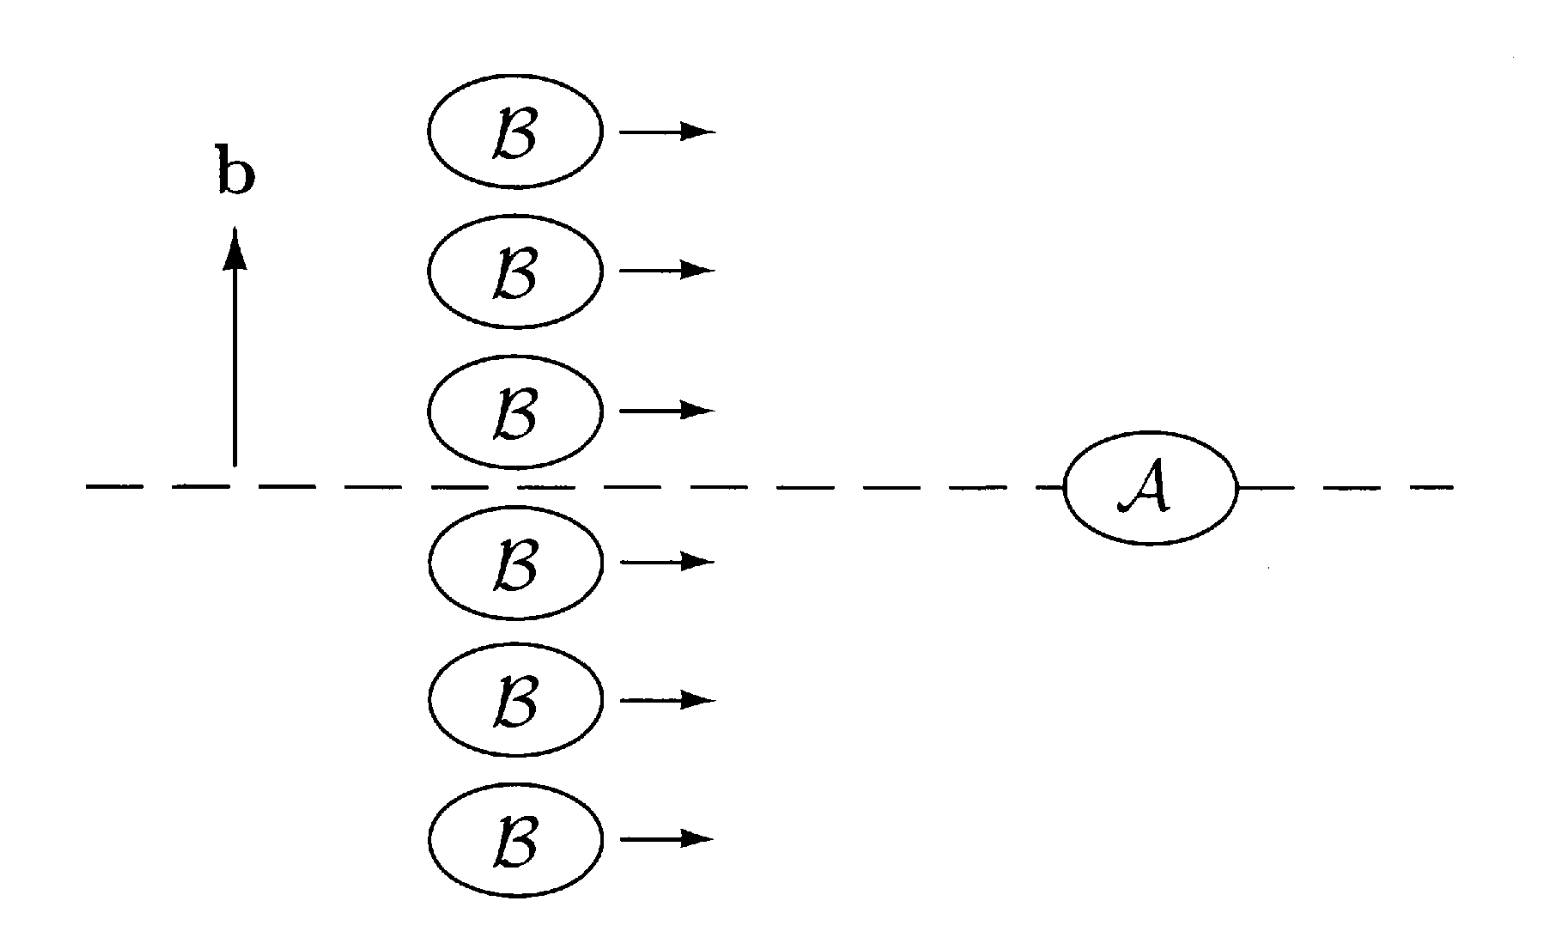
\includegraphics[width=0.6\textwidth]{Peskin_scattering.png}
\caption{\label{scatter}\emph{Incident wavepackets are uniformly distributed in impact parameter $\textbf{b}$.}}
\end{figure}
\item In general we will be considering co-linear interactions (so $b=0$). To account for this fact we will separate the contribution of the momenta of $\phi_{\mathcal{B}}$ along the direction of $\textbf{b}$, this amounts to adding in a factor of $e^{-i\textbf{b}\cdot \textbf{k}_{\mathcal{B}}}$ to the integral expression (as this is the form of the solutions to the Klein Gordon equation) which then takes the form:
\begin{align}
\label{phi_AB}
  \ket{\phi_{\mathcal{A}}\phi_{\mathcal{B}}} = \int\frac{d^3k_{\mathcal{A}}}{(2\pi)^3}\int \frac{d^3k_{\mathcal{B}}}{(2\pi)^3}\frac{\phi_{\mathcal{A}}\phi_{\mathcal{B}}}{2\sqrt{E_{\textbf{k}_{\mathcal{A}}}E_{\textbf{k}_{\mathcal{B}}}}}e^{-i\textbf{b}\cdot \textbf{k}_{\mathcal{B}}}\ket{\textbf{k}_{\mathcal{A}}\textbf{k}_{\mathcal{B}}}
\end{align}
For the out states it is preferable to consider specific momenta $\textbf{p}_i$, so the main object of interest we will need to compute is ${}_{\text{in}}\braket{\textbf{p}_1\textbf{p}_2 \cdot \cdot \cdot|\textbf{k}_{\mathcal{A}}\textbf{k}_{\mathcal{B}}}_{\text{out}}$. But recall that we defined our out states to be in the far future and out in states in the far past, so we must include the limits in this:
\begin{align*}
  {}_{\text{in}}\braket{\textbf{p}_1\textbf{p}_2 \cdot \cdot \cdot|\textbf{k}_{\mathcal{A}}\textbf{k}_{\mathcal{B}}}_{\text{out}} & = \lim_{t \rightarrow \infty} {}_{\text{in}}\braket{\underbrace{\textbf{p}_1\textbf{p}_2 \cdot \cdot \cdot}_{t}|\underbrace{\textbf{k}_{\mathcal{A}}\textbf{k}_{\mathcal{B}}}_{-t}}{}_{\text{out}} \\
  & = \lim_{t \rightarrow \infty}{}_{\text{in}}\braket{\textbf{p}_1\textbf{p}_2 \cdot \cdot \cdot|e^{-iH(2t)}|\textbf{k}_{\mathcal{A}}\textbf{k}_{\mathcal{B}}}_{\text{out}}
\end{align*}
Where in the last line we have added the time evolution operator so that both states are at the same common reference time for this limit. This then brings us to define the $S$ \emph{matrix} as:
\begin{flalign}
\label{S_def}
   {}_{\text{in}}\braket{\textbf{p}_1\textbf{p}_2 \cdot \cdot \cdot|\textbf{k}_{\mathcal{A}}\textbf{k}_{\mathcal{B}}}_{\text{out}} =  \braket{\textbf{p}_1\textbf{p}_2 \cdot \cdot \cdot|S|\textbf{k}_{\mathcal{A}}\textbf{k}_{\mathcal{B}}}
\end{flalign}
\item It is clear that if there no iteration between the particles then the $\hat{S}$ matrix is just the identity. This motivates us to isolate the interacting part of the $\hat{S}$ matrix by defining the $\hat{T}$ \emph{matrix} as:
\begin{align*}
   \hat{S} = \mathbbm{1} + i\hat{T}
 \end{align*} 
\end{itemize}
% subsection the_s_matrix (end)

\subsubsection{Invariant Matrix Element} % (fold)
\label{ssub:invariant_matrix_element}
\begin{itemize}
  \item There are more things we know $S$ should satisfy. It should conserve momenta at each collision, meaning $T$ should contain a delta function $\delta^{(4)}(k_{\mathcal{A}}+k_{\mathcal{B}} - \sum_{f}p_f)$. What is left over as part of $T$ will be known as the \emph{invariant} (as it must be Lorentz invariant) \emph{matrix element} and is denoted with a $\mathcal{M}$. Formally this is defined as:
 \begin{align}
 \label{M_matrix}
   \braket{\textbf{p}_1\textbf{p}_2 \cdot \cdot \cdot|i\hat{T}|\textbf{k}_{\mathcal{A}}\textbf{k}_{\mathcal{B}}} = i(2\pi)^4\delta^{(4)}\left(k_{\mathcal{A}}+k_{\mathcal{B}} - \sum p_f\right)\mathcal{M}(k_{\mathcal{A}},k_{\mathcal{B}} \rightarrow \{p_f\})
 \end{align}

 Where $\mathcal{M}$ depends on the initial and final states as would be expected. 
\end{itemize}
 % subsubsection invariant_matrix_element (end)
  \subsection{2 Particle Scattering} % (fold)
  \label{sub:2_particle_scattering}
  \begin{itemize}
    \item Our next step will be to see how the cross section $\sigma$ depends on $\mathcal{M}$. We will do this infinitesimally, so we start with the probability of the initial state of particles $\mathcal{A}$ and $\mathcal{B}$ scattering into a final state of $n$ particles who's momenta lie in a small region $d^3p_1d^3p_2 \cdot \cdot \cdot d^3p_n$ of the phase space. This probability is given by:
 \begin{align}
 \label{prob_AB}
   \mathcal{P}(\mathcal{A}\mathcal{B}\rightarrow 1~ 2 \ldots n) = \left(\prod_f \frac{d^3p_f}{(2\pi)^3}\frac{1}{2E_f}\right)|{}_{\text{out}}\braket{\textbf{p}_1\cdot \cdot \cdot \textbf{p}_n|\phi_{\mathcal{A}}\phi_{\mathcal{B}}}_{\text{in}}|^2
 \end{align}
 With this the total number of scattering events $N$ will be the sum of this probability over all incident particles, i.e. all the different particles in figure \ref{scatter} with different impact parameters. In the continuity limit when we talk about particle densities this becomes an integral wrt the impact parameter $b$:
 \begin{align}
 \label{no_of_events}
    N =  \sum_{\substack{\text{all incident} \\ \text{particles } i}}\mathcal{P}_i = \int d^2b n_{\mathcal{B}}\mathcal{P}(\textbf{b})
  \end{align} 
  Where $n_{\mathcal{B}}$ is the number density. of $\mathcal{B}$ particles. We will assume that this density is constant and take it out of the integral. This then nicely leads us to the cross section which is defined in \ref{cross}, (where $n_{\mathcal{B}} = \rho_{\mathcal{B}}l_{\mathcal{B}}$ and $A \rho_{\mathcal{A}}l_{\mathcal{A}} = A n_{\mathcal{A}} = N_{\mathcal{A}}$, where $N_{\mathcal{A}}$ is the number of $\mathcal{A}$ partiles which is just $1$ as per our setup.):
  \begin{align*}
    \sigma = \frac{N}{\rho_A\rho_B l_A l_B A} = \frac{N}{n_{\mathcal{B}}N_{\mathcal{A}}} = \frac{N}{n_{\mathcal{B}}} = \int d^2b \mathcal{P}(\textbf{b})
  \end{align*}
  We can then combine this expression with \ref{prob_AB} and \ref{phi_AB} to get the infinitesimal cross section :
  \begin{align}
  \label{dsigma}
     d\sigma = \left(\prod_f \frac{d^3p_f}{(2\pi)^3}\frac{1}{2E_f}\right)&\int d^2b\int\frac{d^3k_{\mathcal{A}}}{(2\pi)^3}\int \frac{d^3k_{\mathcal{B}}}{(2\pi)^3}\int\frac{d^3k'_{\mathcal{A}}}{(2\pi)^3}\int \frac{d^3k'_{\mathcal{B}}}{(2\pi)^3}\frac{\phi_{\mathcal{A}}(\textbf{k}_{\mathcal{A})}\phi_{\mathcal{B}}(\textbf{k}_{\mathcal{B})}}{2\sqrt{E_{\textbf{k}_{\mathcal{A}}}E_{\textbf{k}_{\mathcal{B}}}}}\frac{\phi^{\ast}_{\mathcal{A}}(\textbf{k}'_{\mathcal{A})}\phi^{\ast}_{\mathcal{B}}(\textbf{k}'_{\mathcal{B})}}{2\sqrt{E_{\textbf{k}'_{\mathcal{A}}}E_{\textbf{k}'_{\mathcal{B}}}}} \nonumber \\
     \times & e^{-i\textbf{b}\cdot (\textbf{k}_{\mathcal{B}}-\textbf{k}'_{\mathcal{B}})}\left({}_{\text{out}}\braket{\{\textbf{p}_f\}|\textbf{k}_{\mathcal{A}}\textbf{k}_{\mathcal{B}}}{}_{\text{in}}\right)\left({}_{\text{out}}\braket{\{\textbf{p}_f\}|\textbf{k}'_{\mathcal{A}}\textbf{k}'_{\mathcal{B}}}{}_{\text{in}}\right)^{\ast}
  \end{align}
  Where we have integrals over $k$ and $k'$ as those terms are squared in \ref{prob_AB}. Carrying out he $b$ integral will give us the delta function $\delta^{(2)}(\textbf{k}_{\mathcal{B}}^{\perp}-\textbf{k}_{\mathcal{B}}^{'\perp})$. We can get more delta functions by using the definition of the invariant matrix element defined in \ref{M_matrix}, so we can write the brakets in $d\sigma$ as:
  \begin{align*}
    \left({}_{\text{out}}\braket{\{\textbf{p}_f\}|\textbf{k}_{\mathcal{A}}\textbf{k}_{\mathcal{B}}}{}_{\text{in}}\right) = i(2\pi)^4\delta^{(4)}\left(\textbf{k}_{\mathcal{A}}+\textbf{k}_{\mathcal{B}} - \sum \textbf{p}_f\right)\mathcal{M}(\textbf{k}_{\mathcal{A}},\textbf{k}_{\mathcal{B}} \rightarrow \{\textbf{p}_f\}) \\
    \left({}_{\text{out}}\braket{\{\textbf{p}_f\}|\textbf{k}'_{\mathcal{A}}\textbf{k}'_{\mathcal{B}}}{}_{\text{in}}\right)^{\ast}= -i(2\pi)^4\delta^{(4)}\left(\textbf{k}'_{\mathcal{A}}+\textbf{k}'_{\mathcal{B}} - \sum \textbf{p}_f\right)\mathcal{M}(\textbf{k}'_{\mathcal{A}},\textbf{k}'_{\mathcal{B}} \rightarrow \{\textbf{p}_f\})
  \end{align*}
  The two delta functions in $\delta^{(2)}(\textbf{k}_{\mathcal{B}}^{\perp}-\textbf{k}_{\mathcal{B}}^{'\perp})$ and the $4$ in $\left({}_{\text{out}}\braket{\{\textbf{p}_f\}|\textbf{k}'_{\mathcal{A}}\textbf{k}'_{\mathcal{B}}}{}_{\text{in}}\right)^{\ast}$ allow us to perform all $6$ integrals over $\textbf{k}_{\mathcal{A}}'$ and $\textbf{k}_{\mathcal{B}}'$. The only non-trivial one of these is the $0$th component, which we need to explicitly calculate, we do this with the help of the $z$ component of $k$, which point along the direction of collision:
  \begin{align*}
     &\int dk'^z_{\mathcal{A}}dk'^z_{\mathcal{B}}\delta\left(k'^z_{\mathcal{A}}+k'^z_{\mathcal{A}}-\sum p^z_f\right)\delta(E'_{\mathcal{A}}+E'_{\mathcal{B}}-\sum E_{f}) \\
     & = \int dk'^z_{\mathcal{A}}\delta(\sqrt{k'^2_{\mathcal{A}}+m_{\mathcal{A}}^2}+\sqrt{k'^2_{\mathcal{B}}+m_{\mathcal{B}}^2}-\sum E_{f}) \bigg\vert_{k'^z_{\mathcal{B}} = \sum p_f - k'^z_{\mathcal{A}}}  \\
     & = \frac{1}{|\frac{k'^z_{\mathcal{A}}}{E_{\mathcal{A}}}-\frac{k'^z_{\mathcal{B}}}{E_{\mathcal{B}}}|} = \frac{1}{|v_{\mathcal{A}}-v_{\mathcal{B}}|}
   \end{align*} 
   Where we have used the property of the delta function that:
   \begin{align*}
         &\delta(f(x)) = \frac{1}{|f'(x_0)|}\delta(x-x_0) \\
         \implies  & \delta(E_{\mathcal{A}}(k)+E_{\mathcal{B}}(k) - \sum E_{f}) = \frac{\delta(k-k_0)}{|dE_{\mathcal{A}}/dk+dE_{\mathcal{B}}/dk|}
     \end{align*}
     Where $k_0$ is the $k$ such that $E'_{\mathcal{A}}(k)+E'_{\mathcal{B}}(k)= \sum E_{f}$. All of this allows us to write \ref{dsigma} as:
     \begin{align*}
       d\sigma = \left(\prod_f \frac{d^3p_f}{(2\pi)^3}\frac{1}{2E_f}\right)&\frac{|\mathcal{M}(\textbf{k}'_{\mathcal{A}},\textbf{k}'_{\mathcal{B}} \rightarrow \{\textbf{p}_f\})|^2}{2E_{\mathcal{A}}2E_{\mathcal{B}}|v_{\mathcal{A}}-v_{\mathcal{B}}|}\int\frac{d^3k_{\mathcal{A}}}{(2\pi)^3}\int \frac{d^3k_{\mathcal{B}}}{(2\pi)^3} \\
       &\times |\phi_{\mathcal{A}}(\textbf{k}_{\mathcal{A}})|^2|\phi_{\mathcal{B}}(\textbf{k}_{\mathcal{B}})|^2(2\pi)^4\delta^{(4)}\left(\textbf{k}_{\mathcal{A}}+\textbf{k}_{\mathcal{B}} - \sum \textbf{p}_f\right)
     \end{align*}
     \item The wave-packets that we created as part of the in states, $\phi_{\mathcal{A}}(\textbf{k}_{\mathcal{A}})$ and $\phi_{\mathcal{B}}(\textbf{k}_{\mathcal{B}})$ can be made as resolved as our detectors can be, meaning our detectors cannot resolve the spread of the wave-packets only their central value. We can thus to good approximation replace $\textbf{k}_{\mathcal{A}}$ and $\textbf{k}_{\mathcal{B}}$ by $\textbf{p}_{\mathcal{A}}$ and $\textbf{p}_{\mathcal{B}}$ in the integral and pull the delta function out. The remaining integrals are just the normalization of the wave packets that we had in \ref{packet_norm}, so these go to one and we are left with the following which does not depend on the wave-packets constructed:
     \begin{align}
        d\sigma = \left(\prod_f \frac{d^3p_f}{(2\pi)^3}\frac{1}{2E_f}\right)&\frac{|\mathcal{M}(\textbf{p}_{\mathcal{A}},\textbf{p}_{\mathcal{B}} \rightarrow \{\textbf{p}_f\})|^2}{2E_{\mathcal{A}}2E_{\mathcal{B}}|v_{\mathcal{A}}-v_{\mathcal{B}}|}(2\pi)^4\delta^{(4)}\left(\textbf{p}_{\mathcal{A}}+\textbf{p}_{\mathcal{B}} - \sum \textbf{p}_f\right)
      \end{align} 
      To get to the total cross section we will have to integrate this expression. This amounts to integrating over the phase space of all possible output momentum subject to the constraint of momentum conservation. We will often concisely write this as:
          \begin{align}
          \label{Pi_n}
          \int d\Pi_n = \left(\int \prod _f\frac{d^3p_f}{(2\pi)^32E_f}\right)(2\pi)^4\delta^{(4)}(P - \sum_fp_f)
      \end{align} 
      Where $P$ is the total momenta ($P= p_{\mathcal{A}}+p_{\mathcal{B}}$ in the two particle initial state).
        \end{itemize}

\subsubsection{2 Final Particles} % (fold)
\label{ssub:2_final_particles}
\begin{itemize}
    \item In the case of two final particles, one finds \footnote{For this calculation see pg 10 of my Standard model notes \href{https://tbrosnan12.github.io/documents/Fourth_year/Second_semester/Standard_Model.pdf}{here}}
      \begin{align}
      \label{Pi_2}
        \int \Pi_2= \frac{1}{8\pi}\left(\frac{2|\tilde{\textbf{p}}|}{E_{\text{CM}}}\right)\int\frac{d\Omega}{4\pi} 
      \end{align}
      Where $\tilde{\textbf{p}}$ is the value of $p$ such that $ E_{\mathcal{A}}+E_{\mathcal{B}} = E_{\text{CM}}$. The notable limit is the relativistic one where we send the masses of the scattering particles to $0$ (they are small compared to their energy). This means if $P = (E_{\text{CM}},0) \implies p_{\mathcal{A}}=(E_{\mathcal{A}},\textbf{p}) ~\&~ p_{\mathcal{B}}=(E_{\mathcal{B}},-\textbf{p})$, then in the relativistic limit $E>>m_{\mathcal{A}},m_{\mathcal{B}} \implies E_{\text{CM}} = E_{\mathcal{A}}+E_{\mathcal{B}} \approx |\tilde{\textbf{p}}|+|\tilde{\textbf{p}}| =2|\tilde{\textbf{p}}|$. This makes the factor in brackets of \ref{Pi_2} unity, which allows us to write \ref{dsigma} as:
      \begin{align*}
        \frac{d\sigma}{d\Omega} = \frac{1}{2E_{\mathcal{A}}2E_{\mathcal{B}}|v_{\mathcal{A}}-v_{\mathcal{B}}|}\frac{1}{32\pi^2}|\mathcal{M}(\textbf{p}_{\mathcal{A}},\textbf{p}_{\mathcal{B}} \rightarrow \textbf{p}_1,\textbf{p}_2)|^2
      \end{align*}
      We can then impose that in the massless limit, he particles will move at approximately $v_{\mathcal{A}}=-v_{\mathcal{B}}=1 \implies |v_{\mathcal{A}}-v_{\mathcal{B}}| = 1$ as well as $E_{\mathcal{A}}=E_{\mathcal{B}}=\frac{1}{2}E_{\text{CM}}$, so we finally have the well know result:
      \begin{flalign*}
         \frac{d\sigma}{d\Omega} = \frac{|\mathcal{M}|^2}{64\pi^2E_{\text{CM}}^2}
      \end{flalign*}
\end{itemize}
% subsubsection 2_final_particles (end)
% subsection 2_particle_scattering (end)

\subsection{Decay Rates} % (fold)
\label{sub:decay_rates}
\begin{itemize}
  \item Decay rate is the constant that describes how likely particles are to decay into other particles. The probability for a particle $A$ to decay at a time $t$ is given by $P(t) \propto e^{-\Gamma_{A}t}$. We can think of decaying particles as a scattering process where the single original particle $A$ becomes $n$ final particles, $A \rightarrow 1 +\cdot \cdot \cdot n$. With this consideration we can derive an equation for the differential decay $d\Gamma$ in a similar manner to how we calculated the differential cross section \ref{dsigma}. In this case we only consider a single initial state, so only one wave-packet is considered in \ref{phi_AB}. We also can do this in the rest frame of the decaying particle where the particle energy $E_{A}$ is just $E_A =m_A$. Following this procedure results in:
  \begin{align*}
    d\Gamma_A = \frac{1}{2m_A}|\mathcal{M}(A \rightarrow \{p_f\})|^2d\Pi_n
  \end{align*}
\end{itemize}
% subsection decay_rates (end)

\subsection{S Matrix From Feynman Diagrams} % (fold)
\label{sub:s_matrix_from_feynman_diagrams}
\begin{itemize}
  \item We saw that in equation like \ref{ground_state} we could express the ground state $\ket{\Omega}$ in the interacting picture in terms of the ground state of the free theory $\ket{0}$. We would like to do the same thing for our momenta $\ket{\textbf{k}_{\mathcal{A}}\textbf{k}_{\mathcal{B}}}$. Taking inspiration from \ref{ground_state} we can guess that this will be something like:
  \begin{align}
  \label{k_limit}
    \ket{\textbf{k}_{\mathcal{A}}\textbf{k}_{\mathcal{B}}} \propto \lim_{t\rightarrow\infty(1-i\epsilon)}e^{-iHt}\ket{\textbf{k}_{\mathcal{A}}\textbf{k}_{\mathcal{B}}}_0
  \end{align}
  In the previous case we had that the proportionality factor (which contained all vacuum diagrams) canceled out in the final formula leaving us with just the sum of all diagrams with two external points. We will posit for simplicity that the same happens for this case and that only a subset of the Feynman diagrams will actually contribute to our calculation. It turns out, that through a proper proof which we will not present here, that the only type of diagrams that contribute are called \emph{Connected } \& \emph{ Amputated}. We will explain what these mean soon. 

  \item If we had an expression like \ref{k_limit} then we could use it to write the LHS of the $\hat{S}$ matrix \ref{S_def} as the following:
  \begin{align}
  \label{p_dyson}
     {}_{\text{in}}\braket{\textbf{p}_1\textbf{p}_2|\textbf{k}_{\mathcal{A}}\textbf{k}_{\mathcal{B}}}_{\text{out}} & = \lim_{t\rightarrow\infty(1-i\epsilon)}{}_{0}\bra{\textbf{p}_1\textbf{p}_2 }e^{-iH(2t)}\ket{\textbf{k}_{\mathcal{A}}\textbf{k}_{\mathcal{B}}}_{0} \nonumber\\
     & \propto \lim_{t\rightarrow\infty(1-i\epsilon)}{}_{0}\bra{\textbf{p}_1\textbf{p}_2}T\left\{\text{exp}\left(-i\int_{-t}^{t}dt'H_{I}(t')\right)\right\}\ket{\textbf{k}_{\mathcal{A}}\textbf{k}_{\mathcal{B}}}_{0}
   \end{align} 
   Where in the last step we have used Dyson's formula \ref{dyson}. We can examine the expansion of this exponential in powers of the interaction parameter $\lambda$. At first order this is just the identity which is part of the $\mathbbm{1}$ of $\hat{S} = \mathbbm{1}+i\hat{T}$. Thus this not part of the interaction and does not contribute to the matrix element $\mathcal{M}$, thus we can ignore these in our calculation of $\mathcal{M}$. This term is just the particles translating to the final particles, which can be seen from the Feynman diagrams which take the form: 
   \begin{center}
    \begin{tikzpicture}[scale=1.5]
        % Left diagram (Identity)
        \draw (0,0) -- (0,1);
        \draw (1,0) -- (1,1);
        \node at (0,-0.3) {\(\mathcal{A}\)};
        \node at (1,-0.3) {\(\mathcal{B}\)};
        \node at (0,1.3) {\(1\)};
        \node at (1,1.3) {\(2\)};

        % Plus sign
        \node at (1.75,.5) {\(+\)};

        % Right diagram (Crossing with gap)
        \draw (2.5,0) -- (3.5,1);
        \draw[preaction={draw,white,line width=3pt}] (3.5,0) -- (2.5,1);
        %\draw (3.5,0) -- (2.5,2); % Draw over with original color

        \node at (2.5,-0.3) {\(\mathcal{A}\)};
        \node at (3.5,-0.3) {\(\mathcal{B}\)};
        \node at (2.5,1.3) {\(1\)};
        \node at (3.5,1.3) {\(2\)};
    \end{tikzpicture}
\end{center}

\item We would like to proceed in the same manner as we did in the calculation of the expressions for the n-point correlator. The first step is as usual, we normal order any of the terms we have left, leaving us with some contractions. However, in doing so we quickly run into an issue. Since before our expressions like \ref{ground_state} involved the vacuum $\ket{0}$ we could leverage the fact that the when we split our field into positive and negative frequency components, that they satisfied $\phi_I^+\ket{0} =0$ and $\bra{0}\phi_I^-= 0$. But now since we the kets we are acting on are momentum kets and not the vacuum, these relations no-longer hold. In fact they now do the following:
\begin{align*}
   \phi^{+}_I(x)\ket{\textbf{p}} &= \int \frac{d^3k}{(2\pi)^3}\frac{1}{\sqrt{2E_{\textbf{k}}}}a_{\textbf{k}}e^{-ik \cdot x}\sqrt{2E_{\textbf{p}}}a^{\dagger}_{\textbf{p}}\ket{0} \\
   & = \int \frac{d^3k}{(2\pi)^3}\frac{1}{\sqrt{2E_{\textbf{k}}}}e^{-ik \cdot x}\sqrt{2E_{\textbf{p}}}\delta(\textbf{k}-\textbf{p})\ket{0} \\
   &= e^{-ip\cdot x}\ket{0 }
 \end{align*} 
Having noticed this is the case, we can see that if we have a product of fields $\phi_I(x)$, then once we use one of them to act on the state $\ket{\textbf{p}}$, then the left over fields can be normal ordered and only the contractions kept as usual. With this we are motivated to define the contraction of a field $\phi$ with the momentum ket $\ket{\textbf{p}}$ via:
\begin{align*}
  \wick{\c{\phi_I}(x) \c{\ket{\textbf{p}}}(y)} = e^{-ip\cdot x}\ket{0}, ~~~~~\wick{\c{\bra{\textbf{p}}} \c{\phi_I(x)}(y)} = \bra{0}e^{ip\cdot x}
\end{align*}
So before when we had normal ordered terms we could ignore them as they acted on the vacuum $\ket{0}$ and vanished. But now this is not the case, so in expressions like the expansion of \ref{4wick}, all the terms will contribute not just the fully contracted ones. In fact \ref{4wick} is exactly what we would have in the second term in our expansion of the exponential \ref{p_dyson}. Hence this is a good thing to examine closer as it will contain the first interaction terms. 


In \ref{4wick} there are three types of terms, one term with no contractions $\phi\phi\phi\phi$, $7$ terms with one contraction $\wick{\c{\phi}\c{\phi}}\phi\phi$, and $3$ terms with 2 contractions $\wick{\c{\phi}\c{\phi}\c{\phi}\c{\phi}}$. 

\item \textbf{Case 1:} Before only the $\wick{\c{\phi}\c{\phi}\c{\phi}\c{\phi}}$ terms were important, but now we can actually argue that we should ignore these terms. Since all the $\phi$'s are contracted, it means there are no $\phi's$ left over to contract with any of the momentum kets $\ket{\textbf{p}}$. This essentially means these terms are also part of the $\mathbbm{1}$ in the definition of $\hat{S}$, and do not contribute to $\mathcal{M}$. The Feynman diagram for this term is:
\begin{align*}
    \begin{array}{c}
\begin{tikzpicture}[scale=2.5]
  \begin{pgfonlayer}{nodelayer}
    \node [circle, fill, inner sep=1pt] (0) at (-4, 3) {};
  \end{pgfonlayer}
  \begin{pgfonlayer}{edgelayer}
    \draw [in=135, out=45, loop] (0.center) to ();
    \draw [in=225, out=315, loop] (0.center) to ();
  \end{pgfonlayer}
\end{tikzpicture}
    \end{array} \hspace{-5mm}\times ~~  \left(\begin{array}{c}
        \begin{tikzpicture}
            % Left diagram (Identity)
            \draw (0,0) -- (0,1);
            \draw (1,0) -- (1,1);
            \node at (0,-0.3) {\(\mathcal{A}\)};
            \node at (1,-0.3) {\(\mathcal{B}\)};
            \node at (0,1.3) {\(1\)};
            \node at (1,1.3) {\(2\)};
        \end{tikzpicture}
    \end{array} 
    + \begin{array}{c}
        \begin{tikzpicture}
            % Right diagram (Crossing with gap)
            \draw (0,0) -- (1,1);
            \draw[preaction={draw,white,line width=3pt}] (1,0) -- (0,1);
            \node at (0,-0.3) {\(\mathcal{A}\)};
            \node at (1,-0.3) {\(\mathcal{B}\)};
            \node at (0,1.3) {\(1\)};
            \node at (1,1.3) {\(2\)};
        \end{tikzpicture}
    \end{array}\right)
\end{align*}


\item \textbf{Case 2:} For the $\wick{\c{\phi}\c{\phi}}\phi\phi$ terms, the two uncontracted $\phi$'s are normal ordered, so in terms of creation and annihilation operators we know they will be proportional to $a^{\dagger}a^{\dagger} + 2a^{\dagger}a + aa $. We then use of these $\phi$ to contract with either the initial momentum ket or a final momentum ket. Either way results in us getting an exponential as well as $\ket{0}$ or $\bra{0}$. We can then see that only the middle term in  $a^{\dagger}a^{\dagger} + 2a^{\dagger}a + aa $ will be non-vanishing as the other terms will annihilate the vacuum bra/kets. What we are left to do is come up with a way of drawing this process in our Feynman diagrams. Since we have that one of the $\phi$'s is contracted with both the final and initial kets, it makes sense to define their contraction as an \emph{external line}:
\begin{align*}
  \wick{\c{\phi_I}(x) \c{\ket{\textbf{p}}}(y)} =  \begin{array}{c}
\begin{tikzpicture}[decoration={markings, mark=at position 0.5 with {\arrow{stealth}}}]
    \begin{pgfonlayer}{nodelayer}
        \node [circle, fill, inner sep=1pt] (0) at (0, -1) {};
        \node [style=none] (1) at (-0.5, -1) {};
        \node [style=none] (2) at (-0.5, -0.75) {};
        \node [style=none] (3) at (-0.5, -1.25) {};
        \node [style=none] (4) at (1.75, -1) {};
        \node [style=none] (5) at (0.5, -1) {};
        \node [style=none] (6) at (1, -1.25) {$p$};
        \node [style=none] (7) at (1, -.4) {};
    \end{pgfonlayer}
    \begin{pgfonlayer}{edgelayer}
        % Middle arrow instead of end arrow
        \draw [postaction={decorate}] (4.center) to (5.center);
        \draw (5.center) to (0.center);
        \draw (0.center) to (2.center);
        \draw (0.center) to (1.center);
        \draw (0.center) to (3.center);
    \end{pgfonlayer}
\end{tikzpicture}    
  \end{array}
  , ~~~~~ \wick{\c{\bra{\textbf{p}}} \c{\phi_I(x)}(y)} =  \begin{array}{c}
\begin{tikzpicture}[decoration={markings, mark=at position 0.5 with {\arrow{stealth}}}]
    \begin{pgfonlayer}{nodelayer}
        \node [circle, fill, inner sep=1pt] (0) at (0, -1) {};
        \node [style=none] (1) at (0.5, -1) {};
        \node [style=none] (2) at (0.5, -0.75) {};
        \node [style=none] (3) at (0.5, -1.25) {};
        \node [style=none] (4) at (-1.75, -1) {};
        \node [style=none] (5) at (-0.5, -1) {};
        \node [style=none] (6) at (-1, -1.25) {$p$};
        \node [style=none] (7) at (-1, -.4) {};
    \end{pgfonlayer}
    \begin{pgfonlayer}{edgelayer}
        % Middle arrow instead of end arrow
        \draw [postaction={decorate}] (0.center) to (4.center);
        \draw (5.center) to (0.center);
        \draw (0.center) to (2.center);
        \draw (0.center) to (1.center);
        \draw (0.center) to (3.center);
    \end{pgfonlayer}
\end{tikzpicture}    
  \end{array}
\end{align*}
With this we have $4$ different types of diagrams for the $\wick{\c{\phi}\c{\phi}}\phi\phi$ terms:
\begin{align*}
\begin{array}{c}
    \begin{tikzpicture}[scale=2]
            % Left diagram (Identity)
            \draw (0,0) -- (0,1);
            \draw (.75,0) -- (.75,1);
            \node at (0,-0.3) {\(\mathcal{A}\)};
            \node at (.75,-0.3) {\(\mathcal{B}\)};
            \node at (0,1.3) {\(1\)};
            \node at (.75,1.3) {\(2\)};
            \node (1) at (0,0.5) {};
            \draw [in=135, out=225 , loop] (1.center) to ();
        \end{tikzpicture}
  \end{array}
   ~~+~~
\begin{array}{c}
    \begin{tikzpicture}[scale=2]
            % Left diagram (Identity)
            \draw (0,0) -- (0,1);
            \draw (.75,0) -- (.75,1);
            \node at (0,-0.3) {\(\mathcal{A}\)};
            \node at (.75,-0.3) {\(\mathcal{B}\)};
            \node at (0,1.3) {\(1\)};
            \node at (.75,1.3) {\(2\)};
            \node (1) at (.75,0.5) {};
            \draw [in=45, out=-45 , loop] (1.center) to ();
        \end{tikzpicture}
  \end{array}
  ~~+~~
  \begin{array}{c}
    \begin{tikzpicture}[scale=2]
            % Right diagram (Crossing with gap)
            \draw (0,0) -- (1,1);
            \draw[preaction={draw,white,line width=3pt}] (1,0) -- (0,1);
            \node at (0,-0.3) {\(\mathcal{A}\)};
            \node at (1,-0.3) {\(\mathcal{B}\)};
            \node (1) at (0.25,0.25) {};
            \node at (0,1.3) {\(1\)};
            \node at (1,1.3) {\(2\)};
            \draw [in=90, out=180 , loop] (1.center) to ();
\end{tikzpicture}
  \end{array}
   ~~+~~
  \begin{array}{c}
    \begin{tikzpicture}[scale=2]
            % Right diagram (Crossing with gap)
            \draw (0,0) -- (1,1);
            \draw[preaction={draw,white,line width=3pt}] (1,0) -- (0,1);
            \node at (0,-0.3) {\(\mathcal{A}\)};
            \node at (1,-0.3) {\(\mathcal{B}\)};
            \node (1) at (0.75,0.25) {};
            \node at (0,1.3) {\(1\)};
            \node at (1,1.3) {\(2\)};
            \draw [in=90, out=0 , loop] (1.center) to ();
\end{tikzpicture}
  \end{array}
\end{align*}
From these diagrams we can gather that the first two diagrams are also part of the trivial contribution to the $\hat{S}$ matrix as they involve initial and final states that are identical. From this example we can gather that the only diagrams that contribute to the interaction are \emph{fully connected} diagrams. This is what we meant earlier when we mentioned we will only care about connected diagrams.  

\item \textbf{Case 3:}
\end{itemize}
  
% subsection s_matrix_from_feynman_diagrams (end)





\end{document}

